%杨舒云的实验报告编辑界面,使用了Huanyu Shi,2019级的模板,杨舒云在此拜谢ORZ!

%!TEX program = xelatex
\documentclass[dvipsnames, svgnames,a4paper,11pt]{article}
% ----------------------------------------------------- 
%	加边框的命令
%	参考:https://tex.stackexchange.com/questions/531559/how-to-add-the-page-border-for-first-two-pages-in-latex
\usepackage{tikz}
\usetikzlibrary{calc}
\usepackage{eso-pic}
\AddToShipoutPictureBG{%
\begin{tikzpicture}[overlay,remember picture]
\draw[line width=0.6pt] % 边框粗细
    ($ (current page.north west) + (0.6cm,-0.6cm) $)
    rectangle
    ($ (current page.south east) + (-0.6cm,0.6cm) $); % 边框位置
\end{tikzpicture}}


\usepackage{xcolor}
\definecolor{c1}{HTML}{086173} % 目录颜色 原版为2752C9 紫灰色535AAA 蓝紫色0B0DB7 深蓝色070F94 湖绿色219394 松石灰绿086173
\definecolor{c2}{HTML}{E20129} % 引用颜色 原版\definecolor{c2}{RGB}{190,20,83} 橙色F24729

\usepackage{ctex}
\usepackage[top=28mm,bottom=28mm,left=15mm,right=15mm]{geometry}
\usepackage{hyperref} 
\hypersetup{
	colorlinks,
	linktoc = section, % 超链接位置,选项有section, page, all
	linkcolor = c1, % linkcolor 目录颜色
	citecolor = c1  % citecolor 引用颜色
}
\usepackage{amsmath,enumerate,multirow,float}
\usepackage{tabularx}
\usepackage{tabu}
\usepackage{subfig}
\usepackage{fancyhdr}
\usepackage{graphicx}
\usepackage{wrapfig}  
\usepackage{physics}
\usepackage{appendix}
\usepackage{amsfonts}

%
\usepackage{tcolorbox}
\tcbuselibrary{skins,breakable}
\newtcolorbox{tbox}[2][]{
    colframe=black!70!,
    breakable,
    enhanced,
	boxrule =0.5pt,
    title = {#2},
    fonttitle = \large\kaishu\bfseries,
	drop fuzzy shadow,
    #1
}
\newtcolorbox[auto counter,number within=section]{question}[1][]{
  top=2pt,bottom=2pt,arc=1mm,
  boxrule=0.5pt,
%   frame hidden,
  breakable,
  enhanced, %跨页后不会显示下边框
  coltitle=c1!80!gray,
  colframe=c1,
  colback=c1!3!white,
  drop fuzzy shadow,
  title={思考题~\thetcbcounter:\quad},
  fonttitle=\bfseries,
  attach title to upper,
  #1
}

% ---------------------------------------------------------------------
%	利用cleveref改变引用格式,\cref是引用命令
\usepackage{cleveref}
\crefformat{figure}{#2{\textcolor{c2}{Figure #1}}#3} % 图片的引用格式
\crefformat{equation}{#2{(\textcolor{c2}{#1})}#3} % 公式的引用格式
\crefformat{table}{#2{\textcolor{c2}{Table #1}}#3} % 表格的引用格式


% ---------------------------------------------------------------------
%	页眉页脚设置
\fancypagestyle{plain}{\pagestyle{fancy}}
\pagestyle{fancy}
\lhead{\kaishu 中山大学物理与天文学院\uppercase\expandafter{\romannumeral1}} % 左边页眉,学院 + 课程
\rhead{\kaishu 杨舒云的实验报告} % 右边页眉,实验报告标题
\cfoot{\thepage} % 页脚,中间添加页码


% ---------------------------------------------------------------------
%	对目录、章节标题的设置
\renewcommand{\contentsname}{\centerline{\huge 目录}}
\usepackage{titlesec}
\usepackage{titletoc}
% \titleformat{章节}[形状]{格式}{标题序号}{序号与标题间距}{标题前命令}[标题后命令]
\titleformat{\section}{\centering\LARGE\songti}{}{1em}{}

% ---------------------------------------------------------------------
%   listing代码环境设置
\usepackage{listings}
\lstloadlanguages{python}
\lstdefinestyle{pythonstyle}{
backgroundcolor=\color{gray!5},
language=python,
frameround=tftt,
frame=shadowbox, 
keepspaces=true,
breaklines,
columns=spaceflexible,                   
basicstyle=\ttfamily\small, % 基本文本设置,字体为teletype,大小为scriptsize
keywordstyle=[1]\color{c1}\bfseries, 
keywordstyle=[2]\color{Red!70!black},   
stringstyle=\color{Purple},       
showstringspaces=false,
commentstyle=\ttfamily\scriptsize\color{green!40!black},%注释文本设置,字体为sf,大小为smaller
tabsize=2,
morekeywords={as},
morekeywords=[2]{np, plt, sp},
numbers=left, % 代码行数
numberstyle=\it\tiny\color{gray}, % 代码行数的数字字体设置
stepnumber=1,
rulesepcolor=\color{gray!30!white}
}




% ---------------------------------------------------------------------
%	其他设置
\def\degree{${}^{\circ}$} % 角度
\graphicspath{{./images/}} % 插入图片的相对路径
\allowdisplaybreaks[4]  %允许公式跨页 
\usepackage{lipsum}
\usepackage{adjustbox}
%\usepackage{mathrsfs} % 字体
\captionsetup[figure]{name=Figure} % 图片形式
\captionsetup[table]{name=Table} % 表格形式

\begin{document}
	
	
	
	% 实验报告封面	
	
	% 顶栏
	\begin{table}
		\renewcommand\arraystretch{1.7}
		\begin{tabularx}{\textwidth}{
				|X|X|X|X
				|X|X|X|X|}
			\hline
			\multicolumn{2}{|c|}{预习报告}&\multicolumn{2}{|c|}{实验记录}&\multicolumn{2}{|c|}{分析讨论}&\multicolumn{2}{|c|}{总成绩}\\
			\hline
			\LARGE25 & & \LARGE30 & & \LARGE25 & & \LARGE80 & \\
			\hline
		\end{tabularx}
	\end{table}
	% ---
	
	% 信息栏
	\begin{table}
		\renewcommand\arraystretch{1.7}
		\begin{tabularx}{\textwidth}{|X|X|X|X|}
			\hline
			年级、专业: & 2022级 物理学 &组号: & 2\\
			\hline
			姓名: & 杨舒云  & 学号: & 22344020\\
			\hline
			实验时间: & 2024/3/7 & 教师签名: & \\
			\hline
		\end{tabularx}
	\end{table}
	% ---
	
	% 大标题
	\begin{center}
		\LARGE Lab2-1 \quad 原子的发射和吸收光谱观测分析实验
	\end{center}
	% ---
	
	% 注意事项
	
	% 基本
	\textbf{【实验报告注意事项】}
	\begin{enumerate}
		\item 实验报告由三部分组成:
		\begin{enumerate}
			\item 预习报告:课前认真研读实验讲义,弄清实验原理;实验所需的仪器设备、用具及其使用、完成课前预习思考题;了解实验需要测量的物理量,并根据要求提前准备实验记录表格(可以参考实验报告模板,可以打印)。\textcolor{red}{\textbf{(20分)}}
			\item 实验记录:认真、客观记录实验条件、实验过程中的现象以及数据。实验记录请用珠笔或者钢笔书写并签名(\textcolor{red}{\textbf{用铅笔记录的被认为无效}})。\textcolor{red}{\textbf{保持原始记录,包括写错删除部分,如因误记需要修改记录,必须按规范修改。}}(不得输入电脑打印,但可扫描手记后打印扫描件);离开前请实验教师检查记录并签名。\textcolor{red}{\textbf{(30分)}}
			\item 数据处理及分析讨论:处理实验原始数据(学习仪器使用类型的实验除外),对数据的可靠性和合理性进行分析;按规范呈现数据和结果(图、表),包括数据、图表按顺序编号及其引用;分析物理现象(含回答实验思考题,写出问题思考过程,必要时按规范引用数据);最后得出结论。\textcolor{red}{\textbf{(30分)}}
		\end{enumerate}
		\textbf{实验报告就是将预习报告、实验记录、和数据处理与分析合起来,加上本页封面。\textcolor{red}{(80分)}}
		\item 每次完成实验后的一周内交\textbf{实验报告}(特殊情况不能超过两周)。
	\end{enumerate}
	
	% 安全
	\textbf{【实验安全注意事项】}	
	\begin{enumerate}
		\item 实验中光纤不能过度弯折;
		\item 信号强度不能过饱和值;
		\item 光源长时间通电后会发热,小心烫手,切换光源时务必注意(可等断电冷却后再碰);
		\item 请提前了解光纤光谱仪的基本工作原理与关键参数等。		
	\end{enumerate}
	
	% ---
	
	% 特别鸣谢
	\textbf{【特别鸣谢及模板说明】}	
	
	感谢2019级学长石寰宇为本实验报告提供\LaTeX 模板。\textcolor{red}{\textbf{由于原实验报告模板缺少实验编号,为方便在电脑上整理,故添加自命名编号Lab2-1}}
	% ---
	
	
	
	% 目录
	\clearpage
	\tableofcontents
	\clearpage
	% ---
	
	
	
	% 预习报告	
	
	% 小标题
	\setcounter{section}{0}
	\section{Lab2-1 原子的发射和吸收光谱观测分析实验 \quad\heiti 预习报告}
	% ---
	
	% 实验目的
	\subsection{实验目的}
	\begin{enumerate}
		\item CA3.1 原子发射光谱的观测
		\begin{enumerate}
			\item 学习光纤光谱仪的使用;
			\item 观测钠原子光谱,了解碱金属原子光谱的一般规律;
			\item 观测汞原子光谱,了解中外层电子与原子核相互作用;
			\item 观测多种光源的发射光谱,了解线光谱与连续谱的异同。
		\end{enumerate}
		
		\item CA3.2 原子吸收光谱的观测
		\begin{enumerate}
			\item 调配不同浓度的高锰酸钾水溶液;
			\item 测量高锰酸钾水溶液的紫外-可见吸收光谱,找出吸收峰;
			\item 测量不同浓度高锰酸钾水溶液的紫外-可见吸收光谱,验证比
			尔定律;
			\item 测量不同片数玻璃基板的透过光谱,验证朗伯定律。
		\end{enumerate}
	\end{enumerate}
	% ---
	
	% 仪器用具
	\subsection{仪器用具}
	\begin{table}[htbp]
		\centering
		\renewcommand\arraystretch{1.6}
		% \setlength{\tabcolsep}{10mm}
		\begin{tabular}{|p{0.05\textwidth}|p{0.20\textwidth}|p{0.05\textwidth}|p{0.5\textwidth}|}
			\hline
			编号& 仪器用具名称 & 数量 &  主要参数(型号,测量范围,测量精度等) \\
			\hline
			1& 多种光源 & 1 & 低压汞灯、低压钠灯、手机 \\
			\hline
			2& 光纤 & 1 & 0.75m \\
			\hline
			3& 测控计算机 & 1 & -- \\
			\hline
			4& 光谱观测和分析仪器 & 1 & 光纤导入光栅光谱仪,波长范围200-850nm,分辨率0.25nm \\
			\hline
			5& 高锰酸钾水溶液 & -- & -- \\
			\hline
			6& 玻璃基板 & 1 & -- \\
			\hline
			7& 比色皿 、比色皿支架& 1 & 高度40mm、宽度30mm \\
			\hline
		\end{tabular}
	\end{table}
	% ---
	
	% 原理概述
	\subsection{原理概述}
	
	\subsubsection{CA3.1 原子发射光谱的观测}
	\begin{enumerate}
		\item 碱金属原子光谱
		\begin{enumerate}
			\item 碱金属原子具有相对简单的电子结构,其原子核外只有一个价电子。这个外层电子非常容易被激发到更高的能级,当它返回到低能级时,会发射特定波长的光。这使得碱金属原子的光谱特性与内层电子的结构密切相关。例如,钠原子具有11个电子,其中10个为内层电子,1个为价电子。
			
			\begin{figure}[htbp]
				\centering
				\includegraphics[width=0.5\textwidth]{Lab2_1Gra1.jpg}
				\caption{碱金属原子光谱(图片来源于网络)}
				\label{fig:fig1}
			\end{figure}
			
			\item 碱金属原子光谱中,谱线的波数($\bar{\nu}$)可以通过里德伯公式来表示:
			\[
			\tilde{\nu} = R \left( \frac{1}{n_1^{*2}} - \frac{1}{n_2^{*2}} \right)=\dfrac{R}{(n'-\mu'_{l'})^2}-\dfrac{R}{(n-\mu_{l})^2}
			\]
			其中,$R$是里德伯常数,$n_1^*$和$n_2^*$分别是初始和最终能级的有效量子数。l与l'分别为该量子数决定之能级的轨道量子数;
			$\mu_{l}$与$\mu'_{l'}$分别为始态和终态的量子缺(也称量子改正数,量子亏损)。
			\item 钠原子的光谱中存在四个主要的线系:主线系、尖线系、漫线系和基线系,每个线系对应于不同能级跃迁的光谱线。具体到某一线系,例如主线系,其谱线的波数可以具体表示为上述里德伯公式的特定情况。
			
			对于某一线系谱线的波数公式可写为:
			\[\tilde{\nu} = A_{n'l'}-\dfrac{R}{(n-\mu_{l})^2}\]
			
			所有线系的共同特点包括,随着能级跃迁的增加,谱线趋于密集并向较短的波长方向(紫外区)收敛。同一线系内,愈向短波方向,相邻谱线的波数差愈小,最后趋于一个极限——连续谱与分立谱的边界。这是由于能量愈高,能级愈密,最后趋于连续。在同一线系内,愈向短波方向,谱线强度愈小,原因是能级愈高,将原子从基态激发到那一状态也愈不容易。
			
			不同线系的区别主要在于它们所涉及的能级跃迁不同,导致它们出现在光谱的不同区域,例如,某些线系可能在可见光区域,而其他线系则可能在紫外或红外区域。
			在光谱学中,称主线系的第一组线(双线)为共振线,钠原子的共振线就是有名的黄双线(589.0nm 和 589.6nm)。
			从谱线的外表上看,主线系强度较大,锐线系轮廓清晰,漫线系显得弥漫,一般复双重线连成一片。
		\end{enumerate}
		
		\item 单色仪色散系统:单色仪通过使用色散元件(如棱镜或衍射光栅)将入射光分离成其组成的单色光。色散系统的选择(棱镜或光栅)以及其配置(如光栅的线密度)直接影响到光谱仪的分辨率和可测量的波长范围。
		
		\begin{figure}[htbp]
			\centering
			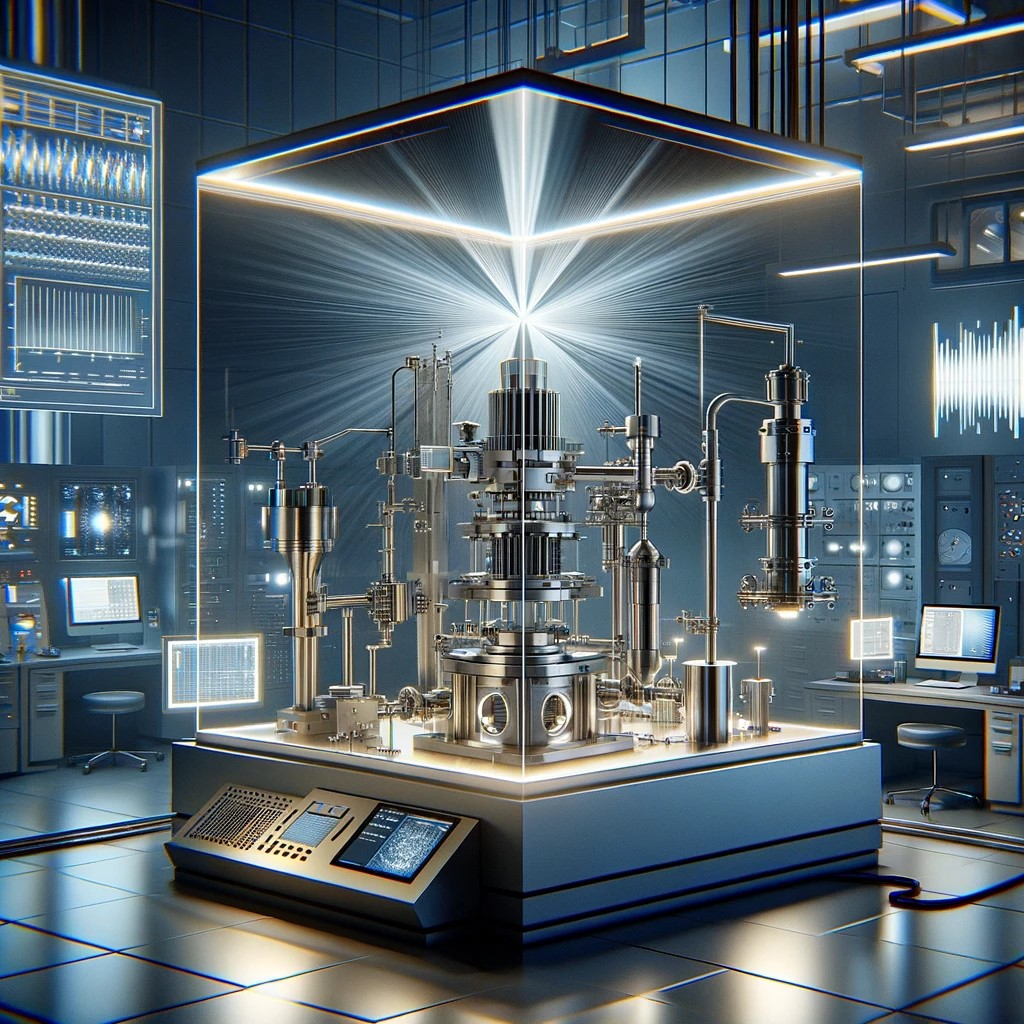
\includegraphics[width=0.4\textwidth]{Lab2_1Gra2.jpg}
			\caption{单色仪色散系统}
			\label{fig:fig2}
		\end{figure}
		
		\item 光谱仪和光学多通道分析仪:光谱仪利用光学元件收集来自样品的发射或吸收光,并通过色散系统对这些光进行分析,从而获得样品的光谱特性。光学多通道分析仪(OMA)是一种高性能的光谱仪,它可以同时收集多个波长的数据,大大提高了数据采集的效率和精度。OMA系统通常包括单色仪、光电探测器(如CCD或CMOS传感器)、以及用于数据处理的计算机系统。
	\end{enumerate}
	
	\subsubsection{CA3.2 原子吸收光谱的观测}
	\begin{enumerate}
		\item 光的吸收
		\begin{enumerate}
			\item 原子和分子吸收光的原理基于量子力学。当原子或分子吸收一定能量的光子时,会从一个能级跃迁到更高的能级。这个过程称为激发态,激发态的原子或分子可以通过辐射或非辐射过程返回到基态,其中辐射过程会发射光子。
			\item Planck公式描述了光子的能量与其频率的关系:
			\[ E = h\nu \]
			其中,\(E\) 是光子的能量,\(h\) 是Planck常数(\(6.62607015 \times 10^{-34}\) J·s),\(\nu\) 是光的频率。
			\item 光的吸收是指当物质(如原子、分子)接收到光能时,使得电子从较低的能级跃迁到较高的能级的过程。这一过程导致特定波长的光减弱,表现为吸收光谱。光的吸收也是指光经过物质时,部分光能被物质吸收,导致通过物质的光强度减弱的现象。这一过程与物质中的原子、分子能级结构有关,只有当光子能量与原子或分子能级差相匹配时,吸收才会发生。
			
			不同波长的光被吸收的特性取决于物质的电子结构(不同波长的光被吸收的特性取决于原子或分子能级结构的差异)。不同原子或分子根据其能级差异,会吸收不同波长(或频率)的光。每种原子或分子只吸收特定波长(即能量)的光,这些特定的波长对应于原子或分子内部能级之间的能量差。这种特性使得吸收光谱能够作为识别和分析化学物质的重要工具。因此,通过分析样品对不同波长光的吸收特性,可以得知样品中含有哪些元素。
		\end{enumerate}
		
		\item Lambert定律
		\begin{enumerate}
			\item Lambert定律描述了描述了无色散介质中光强度随穿过物质厚度的指数衰减规律,表明光的吸收与通过介质的路径长度成正比。
			
			\begin{figure}[htbp]
				\centering
				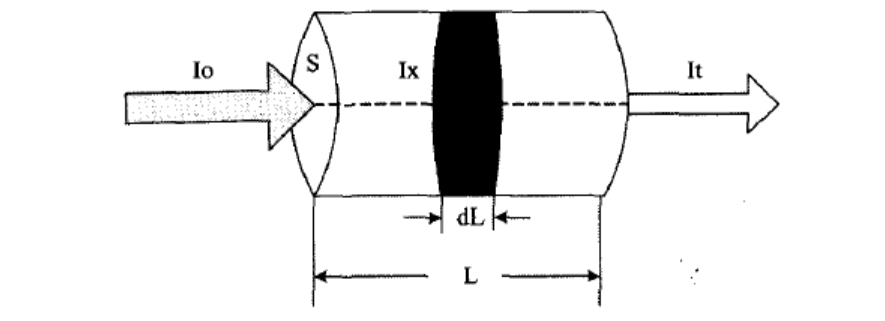
\includegraphics[width=0.45\textwidth]{Lab2_1Gra3.png}
				\caption{Lambert定律}
				\label{fig:fig3}
			\end{figure}
			
			\item Lambert定律的数学表达式为:
			\[ I = I_0 e^{-\alpha l} \]
			其中,\(I\) 是经过物质后的光强,\(I_0\) 是初始光强,\(\alpha\) 是吸收系数,\(l\) 是光通过物质的长度。
		\end{enumerate}
		
		\item Beer定律
		\begin{enumerate}
			\item Beer定律描述了溶液的浓度与它吸收特定波长光的能力之间的关系,表明吸收强度与溶质的浓度成正比。
			
			\begin{figure}[htbp]
				\centering
				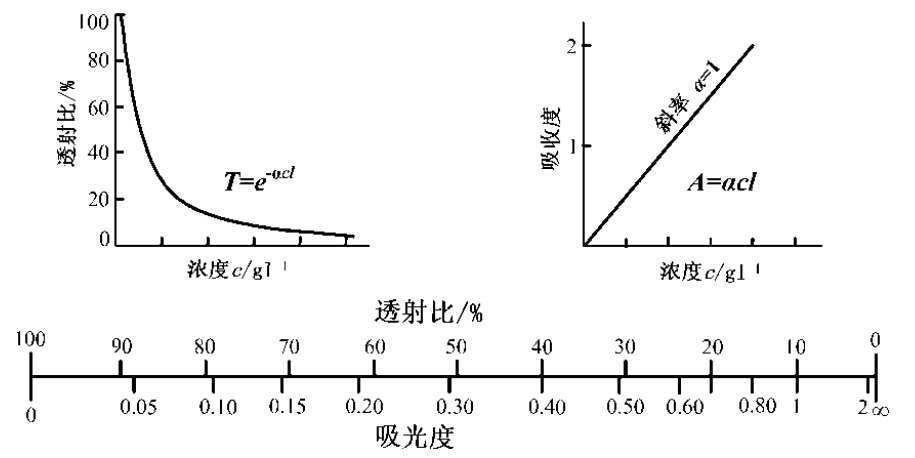
\includegraphics[width=0.6\textwidth]{Lab2_1Gra4.png}
				\caption{Beer定律}
				\label{fig:fig4}
			\end{figure}
			
			\item Beer定律的数学表达式为:
			\[ A = \epsilon c l \]
			其中,\(A\) 是吸光度,\(\epsilon\) 是摩尔吸光系数,\(c\) 是溶质的浓度,\(l\) 是光通过溶液的路径长度。
		\end{enumerate}
		
		\item 结合Lambert定律和Beer定律,我们得到Lambert-Beer定律:
		\[ A = \epsilon c l = \log \frac{I_0}{I} \]
		这表明吸光度与经过介质后的光强比的对数成正比,是分析化学中定量分析物质浓度的基础公式。
		
		\begin{figure}[htbp]
			\centering
			\subfloat[]{
				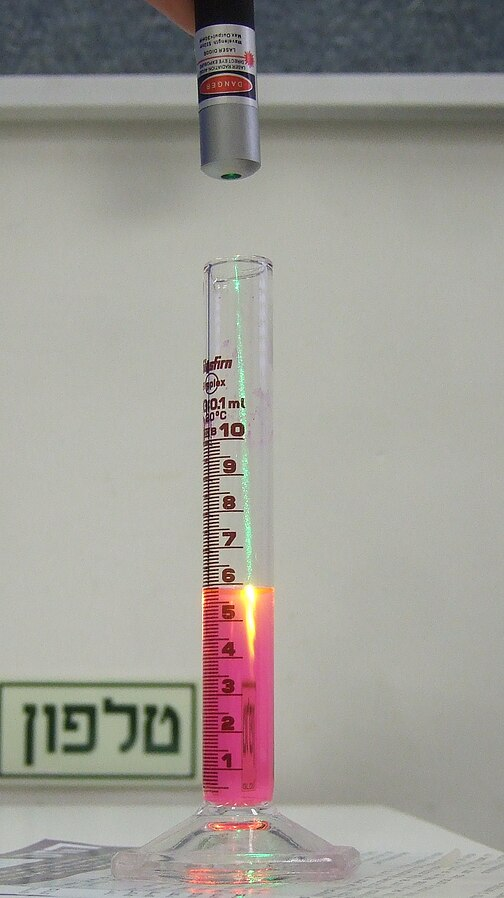
\includegraphics[width=0.2\textwidth]{Lab2_1Gra5.jpg}
			}
			\subfloat[]{
				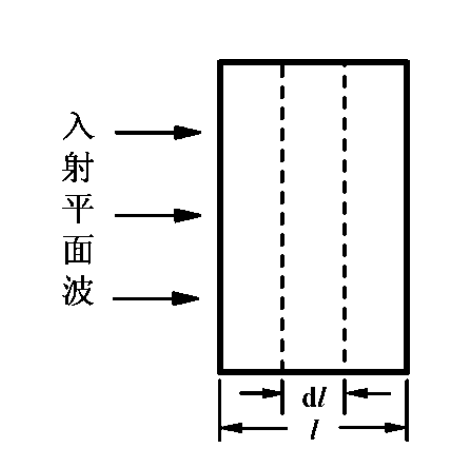
\includegraphics[width=0.4\textwidth]{Lab2_1Gra6.png}
			}
			\caption{Lambert-Beer定律}
			\label{fig:fig5}			
		\end{figure}
		
	\end{enumerate}
	% ---
	
	
	
	% 实验前思考题
	\subsection{实验前思考题}
	
	% 思考题1
	\begin{question}
		日常生活中,光源可以分为热光源和冷光源,请分别说明太阳光、蜡烛、白炽灯、荧光灯、 LED 灯等属于哪一类光源,为什么?
	\end{question}
	在日常生活中,光源可以分为热光源和冷光源两大类。这一分类基于光源发光的物理原理和其发出光的特性。以下是对几种光源的归类及其原因的解释:
	
	\begin{enumerate}
		\item 太阳光:太阳光是一种自然的热光源。它来自太阳的热辐射,太阳表面的高温使得其能够发出光线和热量。
		\item 蜡烛:蜡烛属于热光源。当蜡烛燃烧时,其产生的热量使得蜡烛的燃料发光,产生光线。
		\item 白炽灯:白炽灯是热光源的一种。它通过电流加热灯丝(通常是钨丝),使其达到高温并发光。这种光源的特点是大部分能量以热量的形式散失。
		\item 荧光灯:荧光灯属于冷光源。它使用电流激发气体或汞蒸气产生紫外光,紫外光随后激发涂在灯管内壁的荧光粉发出可见光。相比于白炽灯,荧光灯的热量释放较少,效率更高。
		\item LED灯:LED灯是冷光源。它通过半导体材料在电流作用下直接产生光,其转换效率高,发热量低,因此被认为是冷光源。
	\end{enumerate}
	
	总结如下,太阳光、蜡烛和白炽灯属于热光源,因为它们的光主要通过物质加热发出;而荧光灯和LED灯则是冷光源,这是因为它们通过电子激发而非加热产生光。每种光源的特点和应用场景不同,选择合适的光源可以根据具体需求和能效来决定。
	
	
	% ---
	
	
	
	% 实验记录	
	\clearpage
	
	% 顶栏
	\begin{table}
		\renewcommand\arraystretch{1.7}
		\centering
		\begin{tabularx}{\textwidth}{|X|X|X|X|}
			\hline
			专业: & 物理学 & 年级: & 2022级 \\
			\hline
			姓名: & 杨舒云 & 学号: & 22344020\\
			\hline
			室温:15\degree C &  & 实验地点:A501 &  \\
			\hline
			学生签名:& 杨舒云 & 评分: &\\
			\hline
			实验时间:& 2024/3/7 & 教师签名:&\\
			\hline
		\end{tabularx}
	\end{table}
	% ---
	
	% 小标题
	\section{Lab2-1 原子的发射和吸收光谱观测分析实验  \quad\heiti 实验记录}
	% ---
	
	% 实验过程记录
	\subsection{实验内容、步骤与结果}
	
	%
	\subsubsection{操作步骤记录}
	\begin{enumerate}
		\item \textbf{CA3.1 原子发射光谱的观测}实验操作步骤:
		\begin{enumerate}
			\item 正确连接光谱仪和光源。
			\item 打开软件,确认光谱仪连接正确。
			\item 打开光源,开始测量,自动设置积分时间,再手动调整积分时间和平均次数。
			\item 调整信号强度至饱和值的80%左右。
			\item 分别测量钠灯、汞灯的光谱,并保存光谱图片和实验数据。
			\item 观测记录实验室电灯(改为手机闪光灯)、手机屏光谱,分析光谱特点。
		\end{enumerate}
				
		\item \textbf{CA3.2 原子吸收光谱的观测}实验操作步骤:
		\begin{enumerate}
			\item 准备不同浓度的高锰酸钾溶液。
			\item 正确链接光谱仪和光源,放置纯水样品进行测试。
			\item 打开软件,确认光谱仪连接正确。
			\item 打开光源,开始测量,自动设置积分时间,再手动调整。
			\item 存储参考背景和暗背景。
			\item 更换样品,测量吸收光谱。
			\item 选择吸光度模式,实时显示测量结果,并保存数据。
			\item 对比之前保存的实验数据。
			\item 验证比尔定律,测量记录各种浓度的高锰酸钾溶液吸收曲线,并找出吸收峰波长。
			\item 验证朗伯定律,记录不同片数玻璃基板的透过光谱曲线,分析透过率与玻璃基板厚度的关系。
		\end{enumerate}
	\end{enumerate}	
	
	%
	\subsubsection{实验数据记录}
	\begin{enumerate}
		\item 钠灯光谱
		
		对钠灯谱线进行了多次测量,并标注出了其特征谱线,如\cref{fig:figA1}和\cref{fig:figA2}所示,更进一步的解读与分析见\textbf{数据分析}部分。
		
		\begin{figure}[htbp]
			\centering
			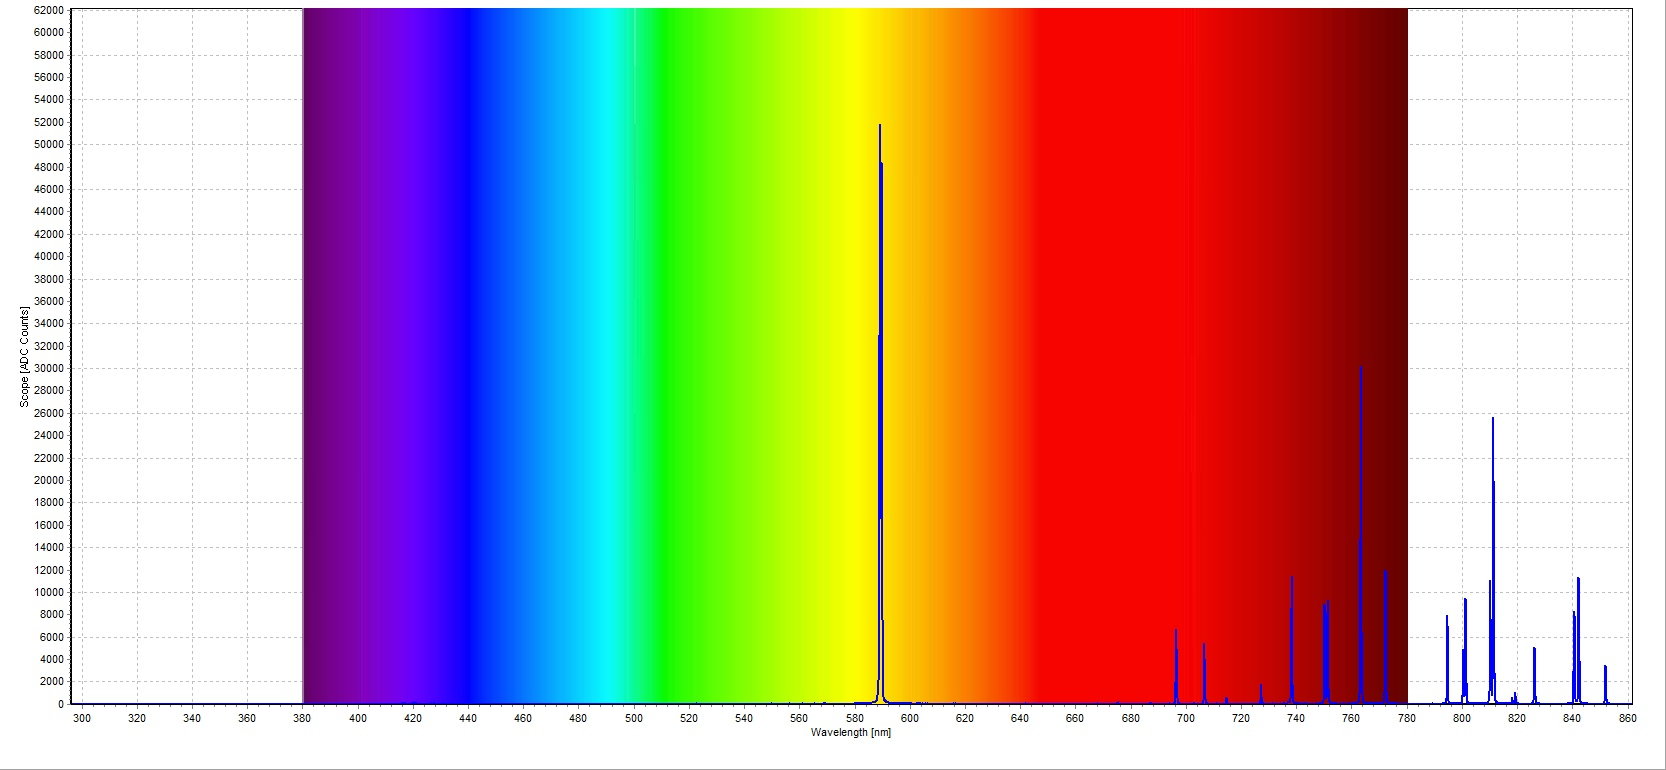
\includegraphics[width=0.6\textwidth]{Lab2_1Gra_A_Na1.jpg}
			\caption{钠灯谱线1}
			\label{fig:figA1}
		\end{figure}
		
		\begin{figure}[htbp]
			\centering
			\subfloat[]{
				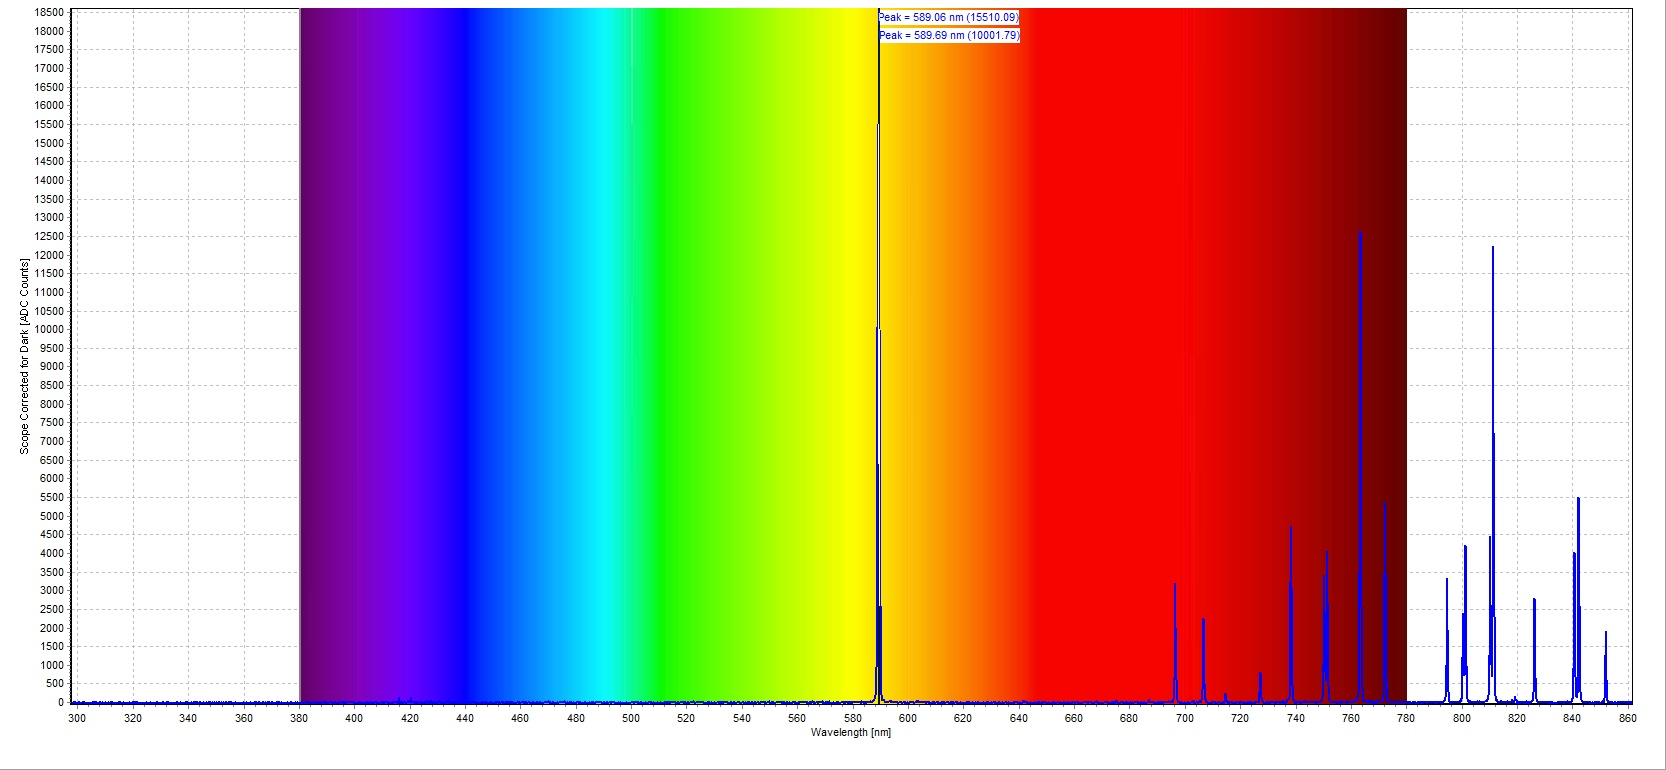
\includegraphics[width=0.4\textwidth]{Lab2_1Gra_A_Na2.jpg}
			}
			\subfloat[]{
				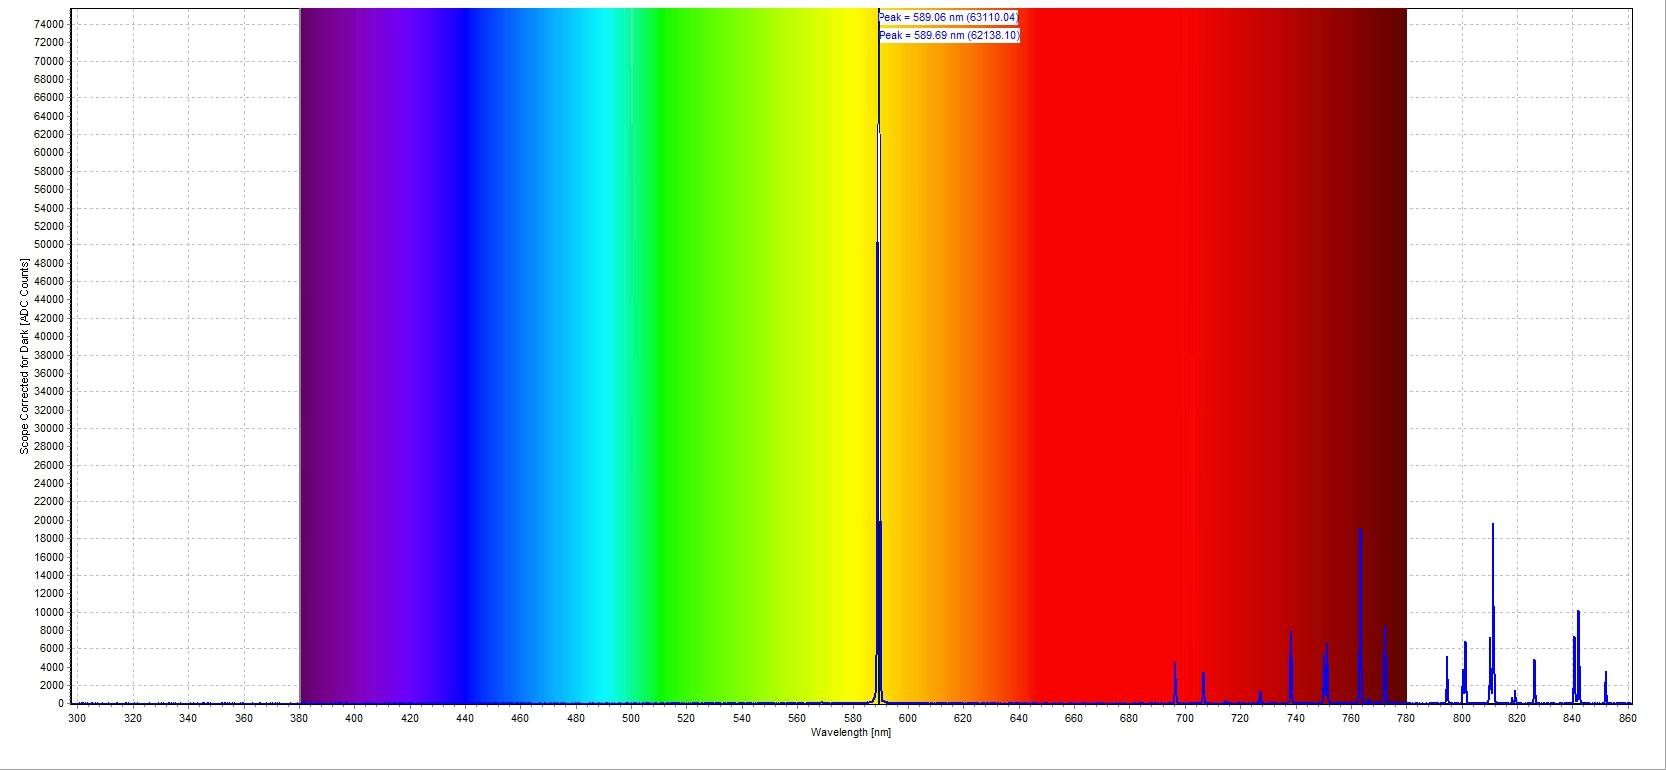
\includegraphics[width=0.4\textwidth]{Lab2_1Gra_A_Na3.jpg}
			}
			\caption{钠灯谱线2}
			\label{fig:figA2}			
		\end{figure}
		
		\begin{figure}[htbp]
			\centering
			\subfloat[]{
				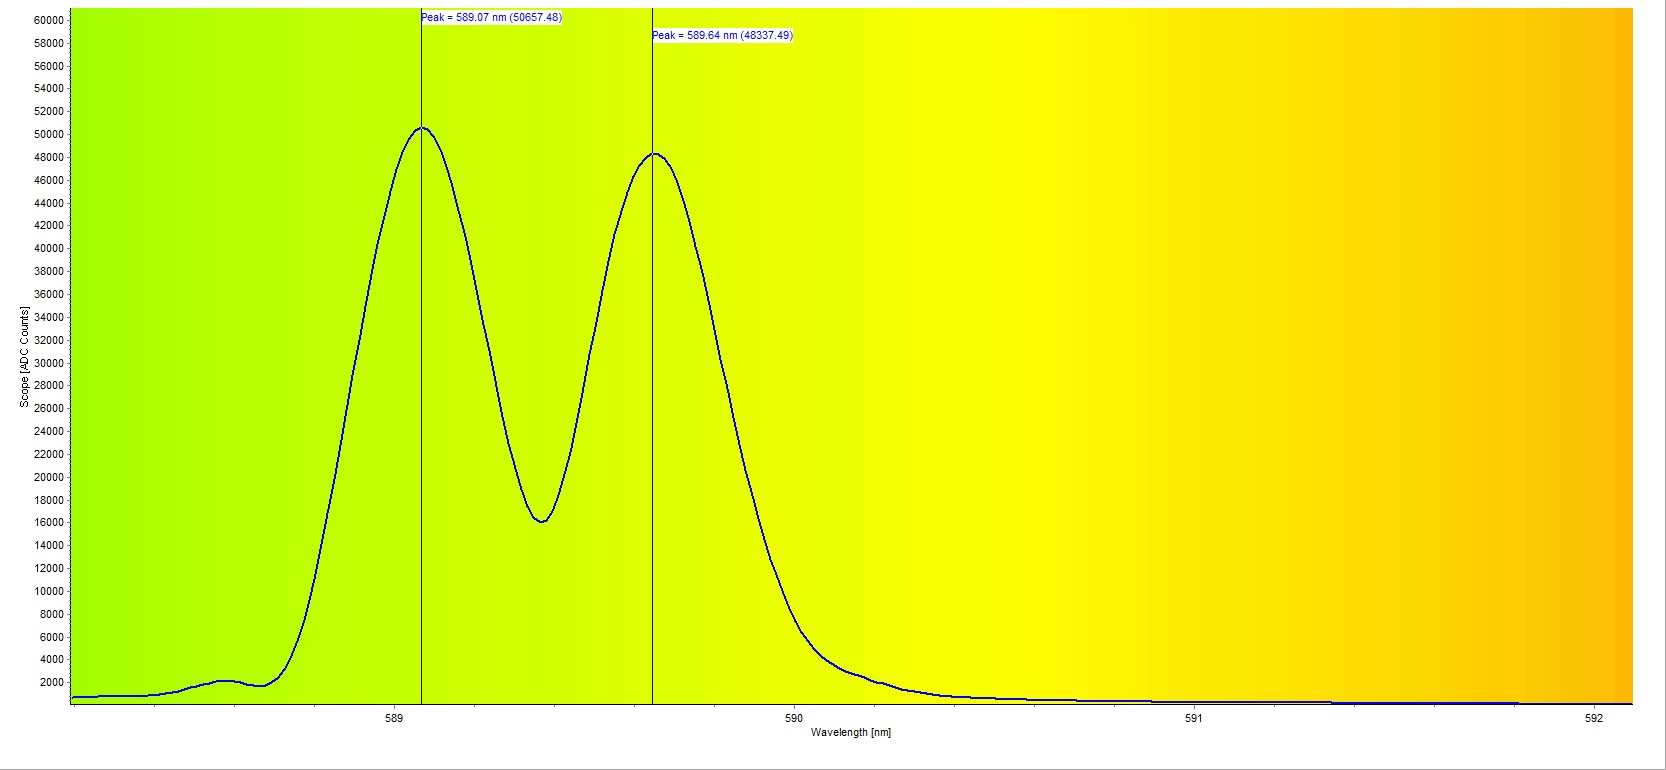
\includegraphics[width=0.45\textwidth]{Lab2_1Gra_A_Na1DY.jpg}
			}
			\subfloat[]{
				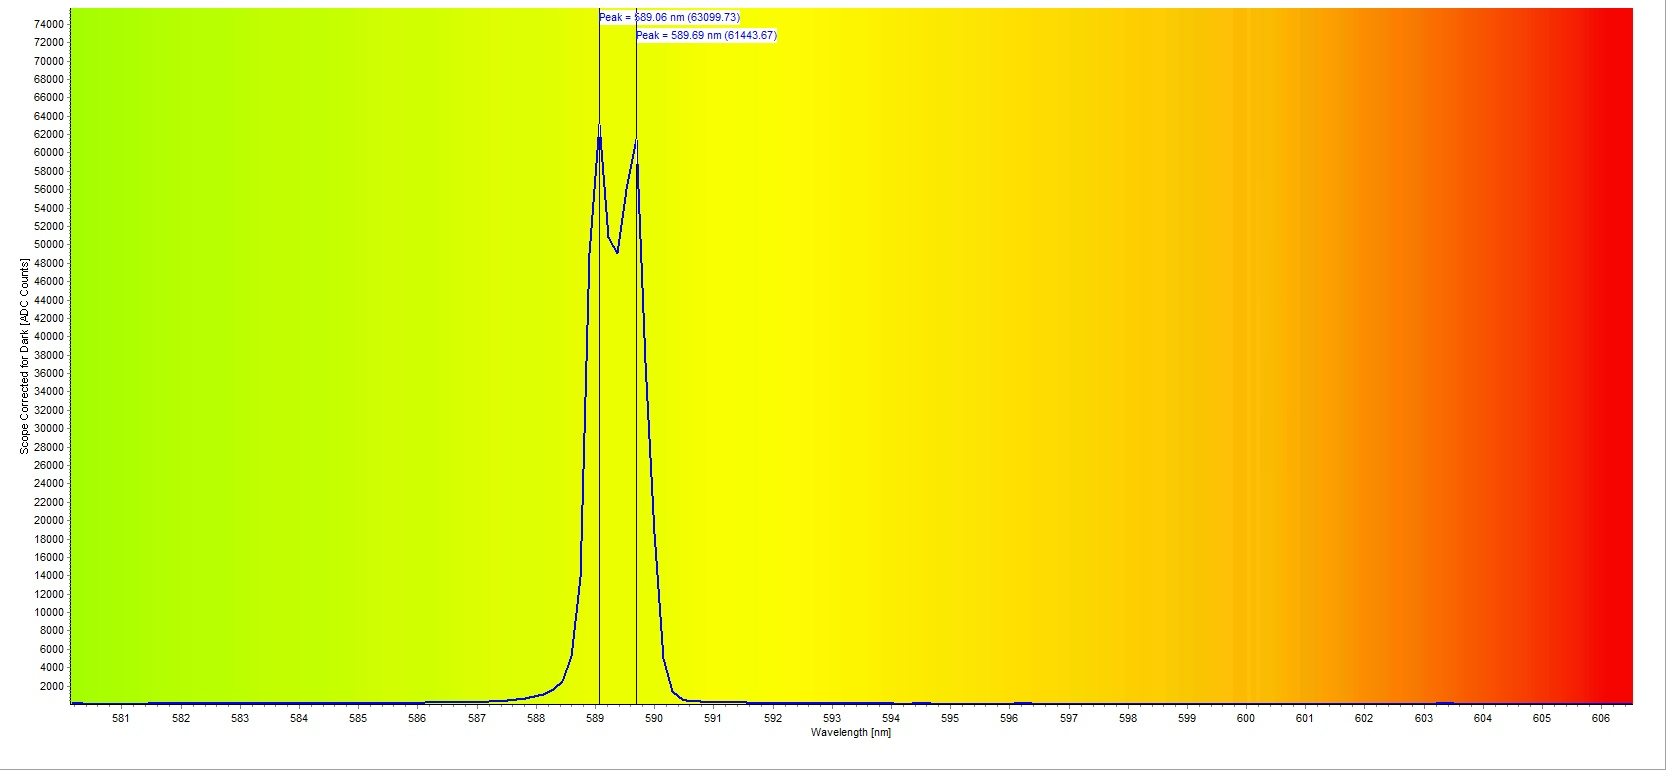
\includegraphics[width=0.45\textwidth]{Lab2_1Gra_A_Na2DY.jpg}
			}
			\caption{钠灯特征谱线}
			\label{fig:figA3}			
		\end{figure}
		
		\item 汞灯光谱
		
		对汞灯谱线进行了多次测量,并标注出了其特征谱线,如\cref{fig:figA4}和\cref{fig:figA5}所示,更进一步的解读与分析见\textbf{数据分析}部分。
		
		\begin{figure}[htbp]
			\centering
			\subfloat[]{
				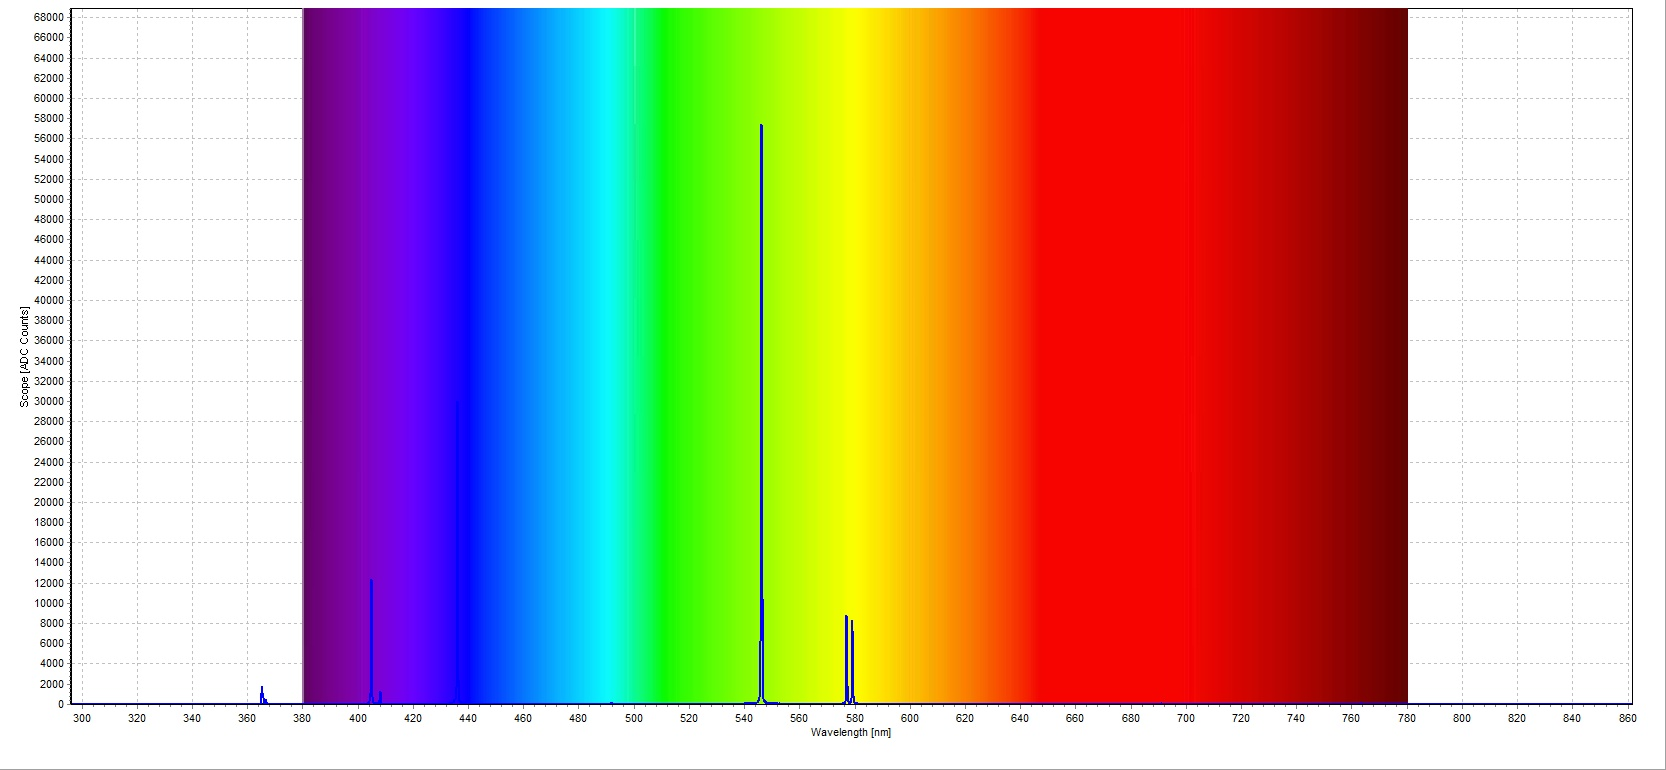
\includegraphics[width=0.45\textwidth]{Lab2_1Gra_A_Hg1.jpg}
			}
			\subfloat[]{
				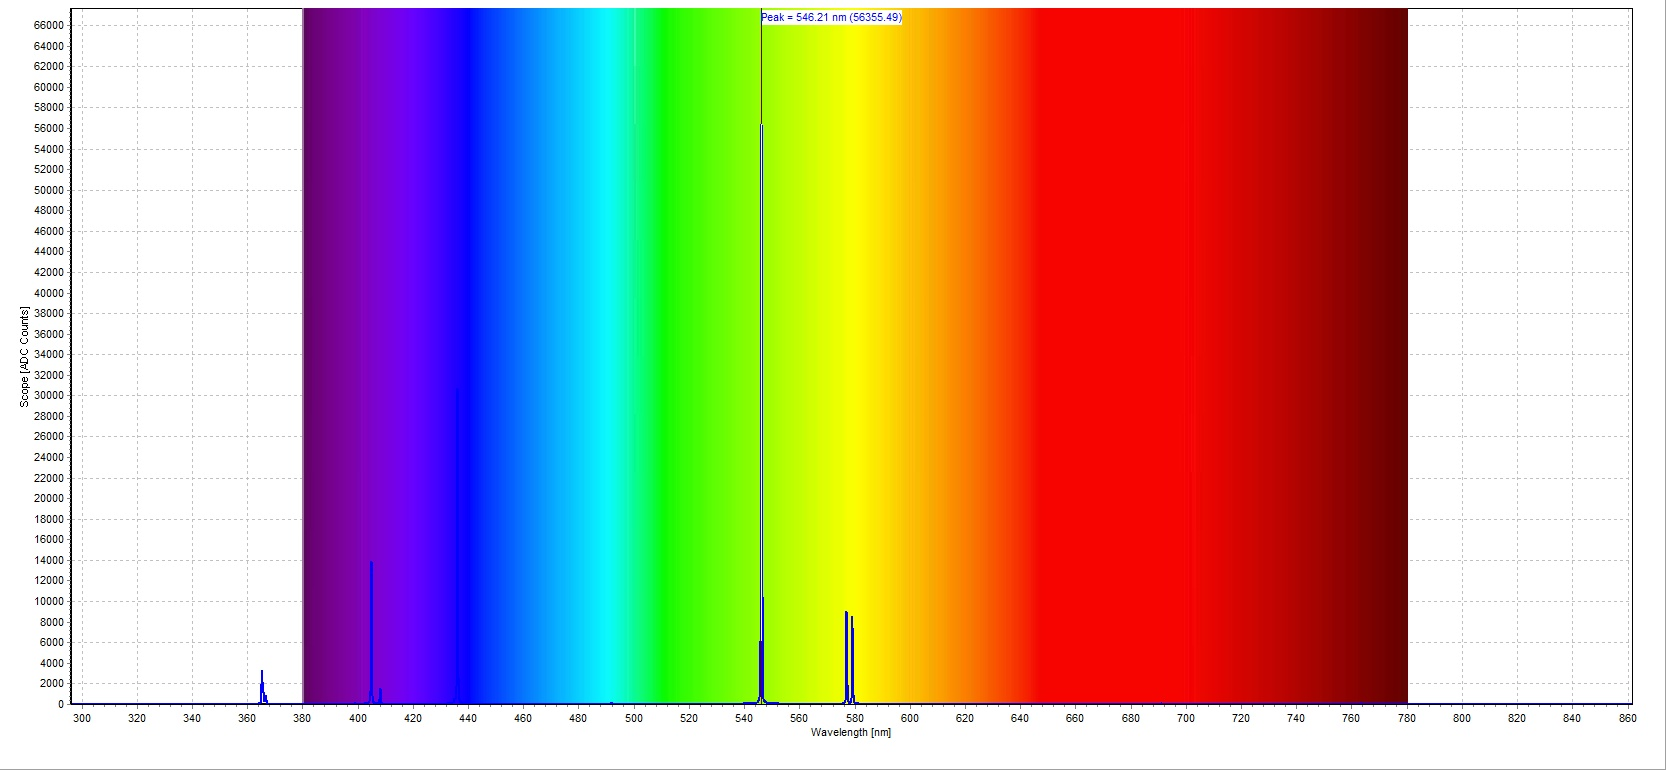
\includegraphics[width=0.45\textwidth]{Lab2_1Gra_A_Hg2.jpg}
			}
			\caption{汞灯谱线}
			\label{fig:figA4}			
		\end{figure}
		
		\begin{figure}[htbp]
			\centering
			\subfloat[]{
				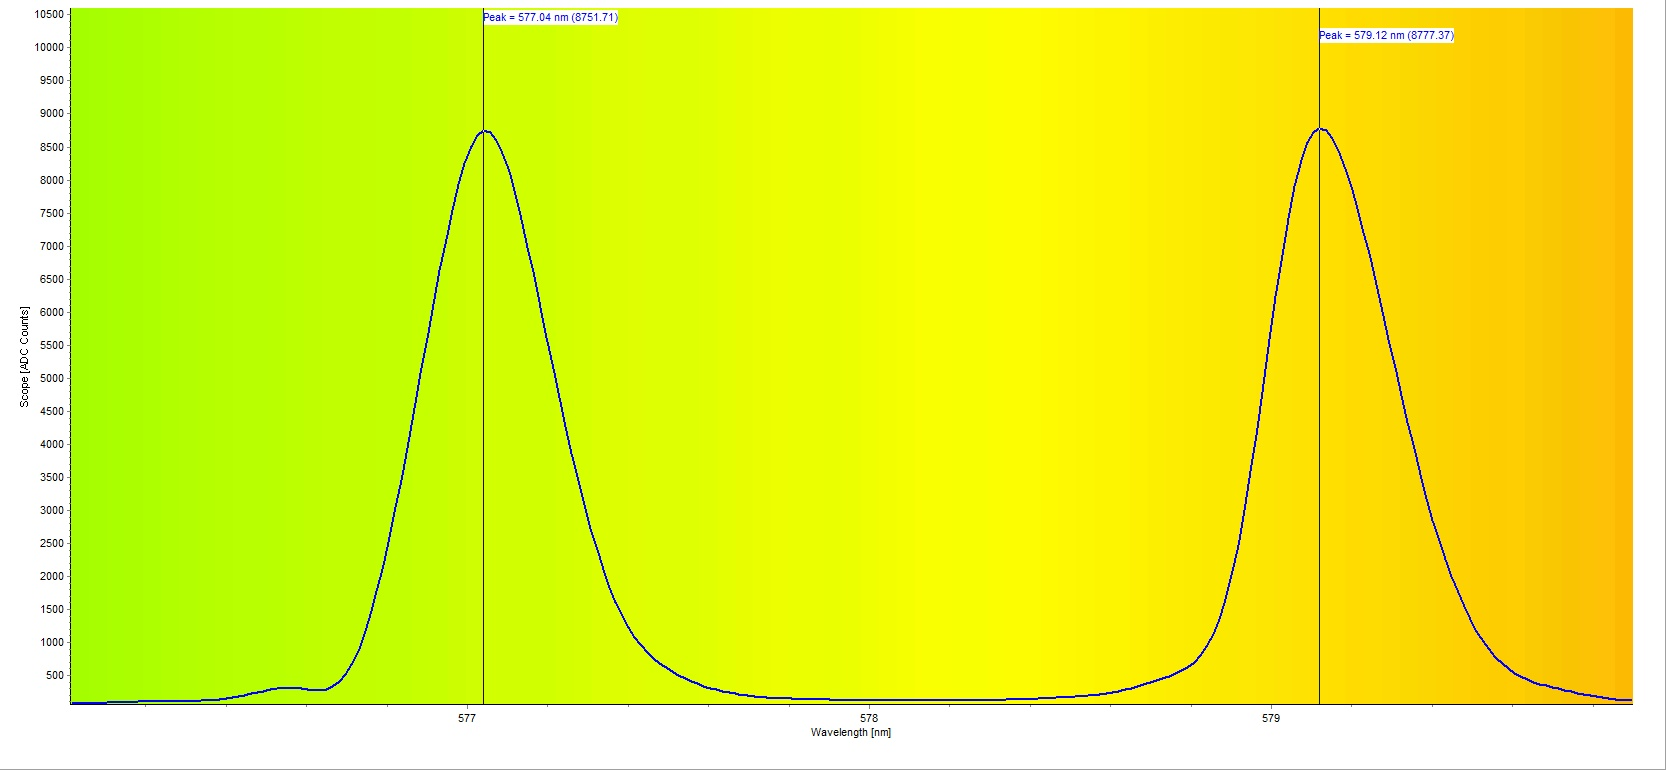
\includegraphics[width=0.45\textwidth]{Lab2_1Gra_A_HgDP.jpg}
			}
			\subfloat[]{
				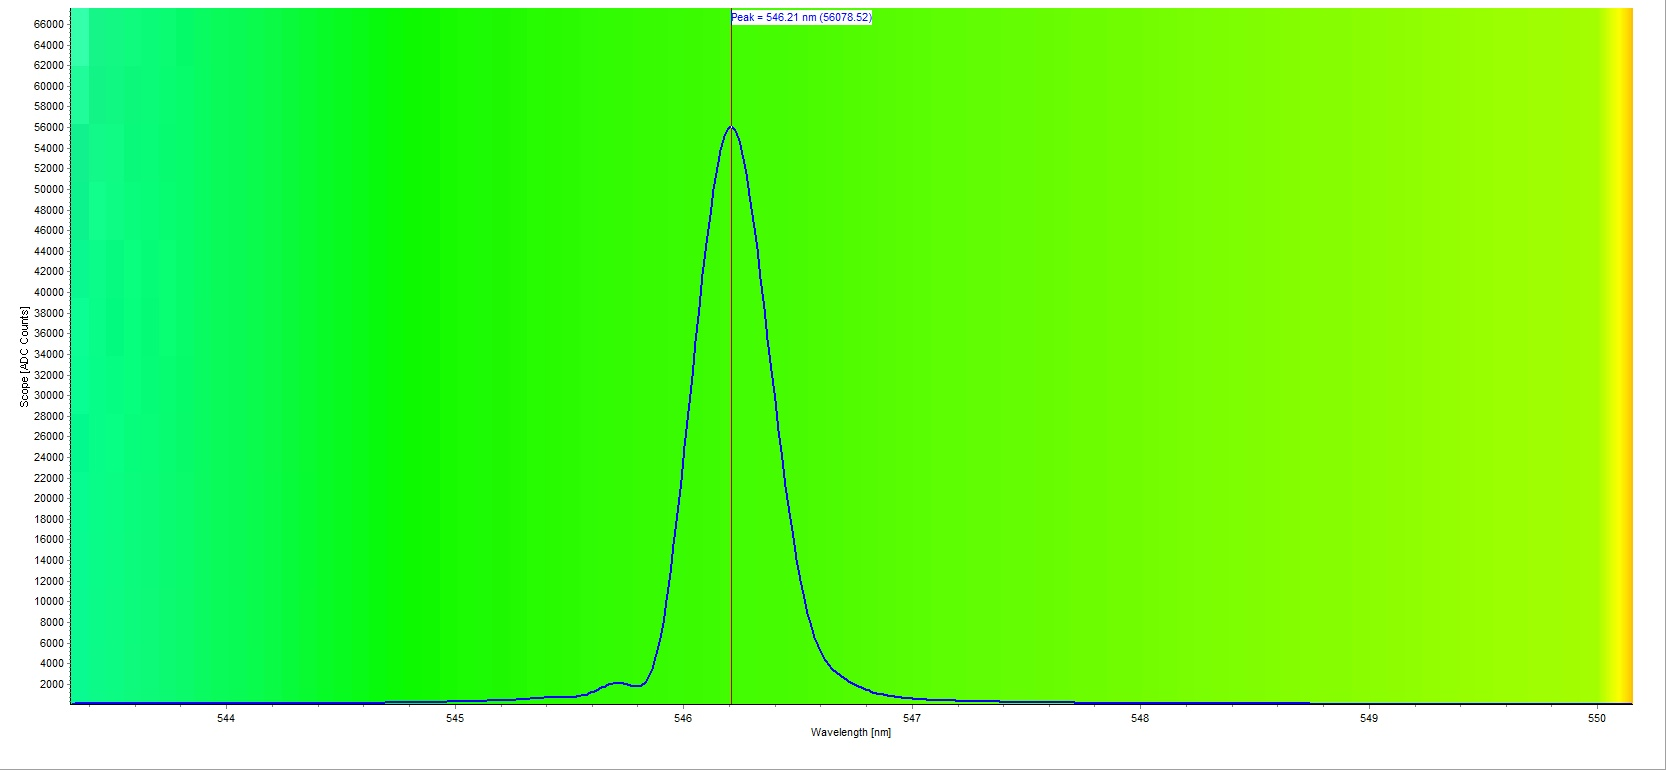
\includegraphics[width=0.45\textwidth]{Lab2_1Gra_A_HgP.jpg}
			}
			\caption{汞灯特征谱线}
			\label{fig:figA5}			
		\end{figure}
		
		\item 手机屏光谱
		
		测量了手机iPhone 13 mini的屏幕光谱,如\cref{fig:figA6}所示,更进一步的解读与分析见\textbf{数据分析}部分。
		
		\begin{figure}[htbp]
			\centering
			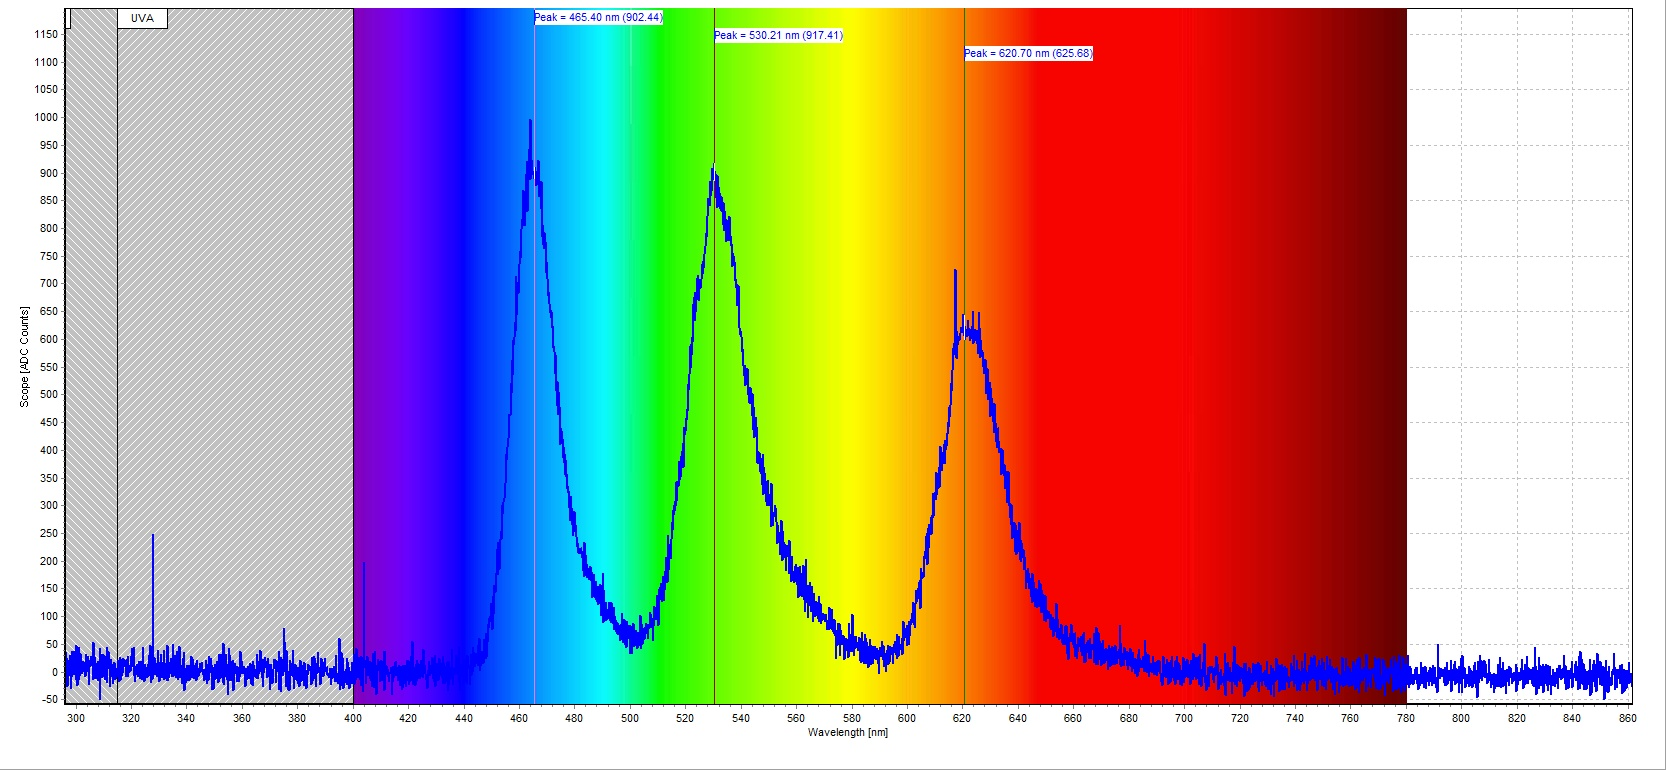
\includegraphics[width=0.6\textwidth]{Lab2_1Gra_A_phone1.jpg}
			\caption{手机屏光谱}
			\label{fig:figA6}
		\end{figure}
		
		\clearpage
		\item 电灯和手机闪光灯光谱
		
		首先,我测量了实验室电灯的发光光谱,发现效果并不太好,如\cref{fig:figA7}所示;
		
		\begin{figure}[htbp]
			\centering
			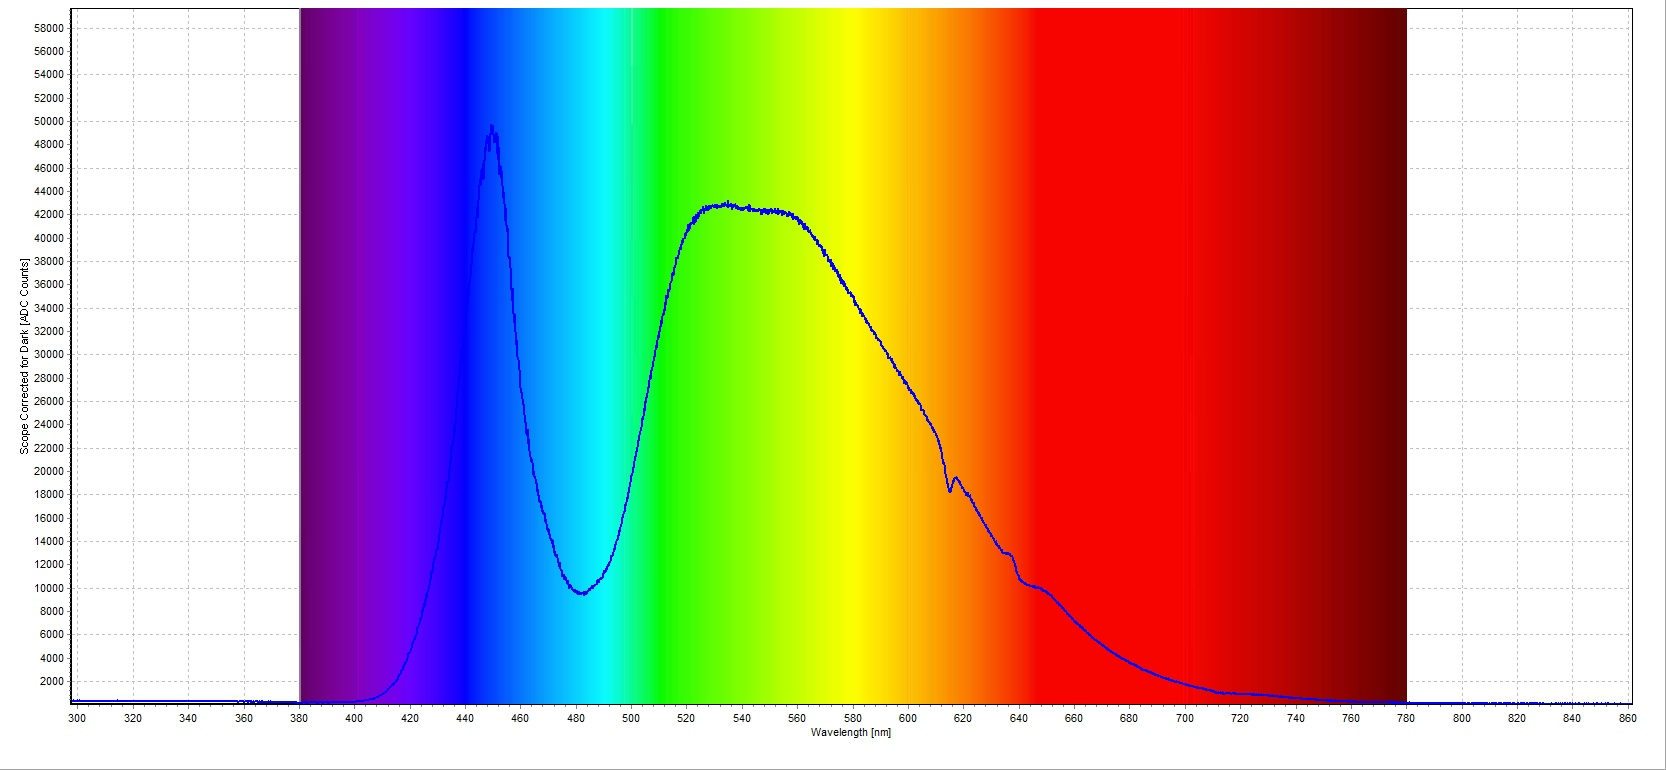
\includegraphics[width=0.9\textwidth]{Lab2_1Gra_A_light.jpg}
			\caption{实验室电灯的发光光谱}
			\label{fig:figA7}
		\end{figure}
		
		接着,出于兴趣和探究精神,我测量了手机闪光灯的发光光谱,如\cref{fig:figA8}所示,更进一步的解读与分析见\textbf{数据分析}部分。
		
		\begin{figure}[htbp]
			\centering
			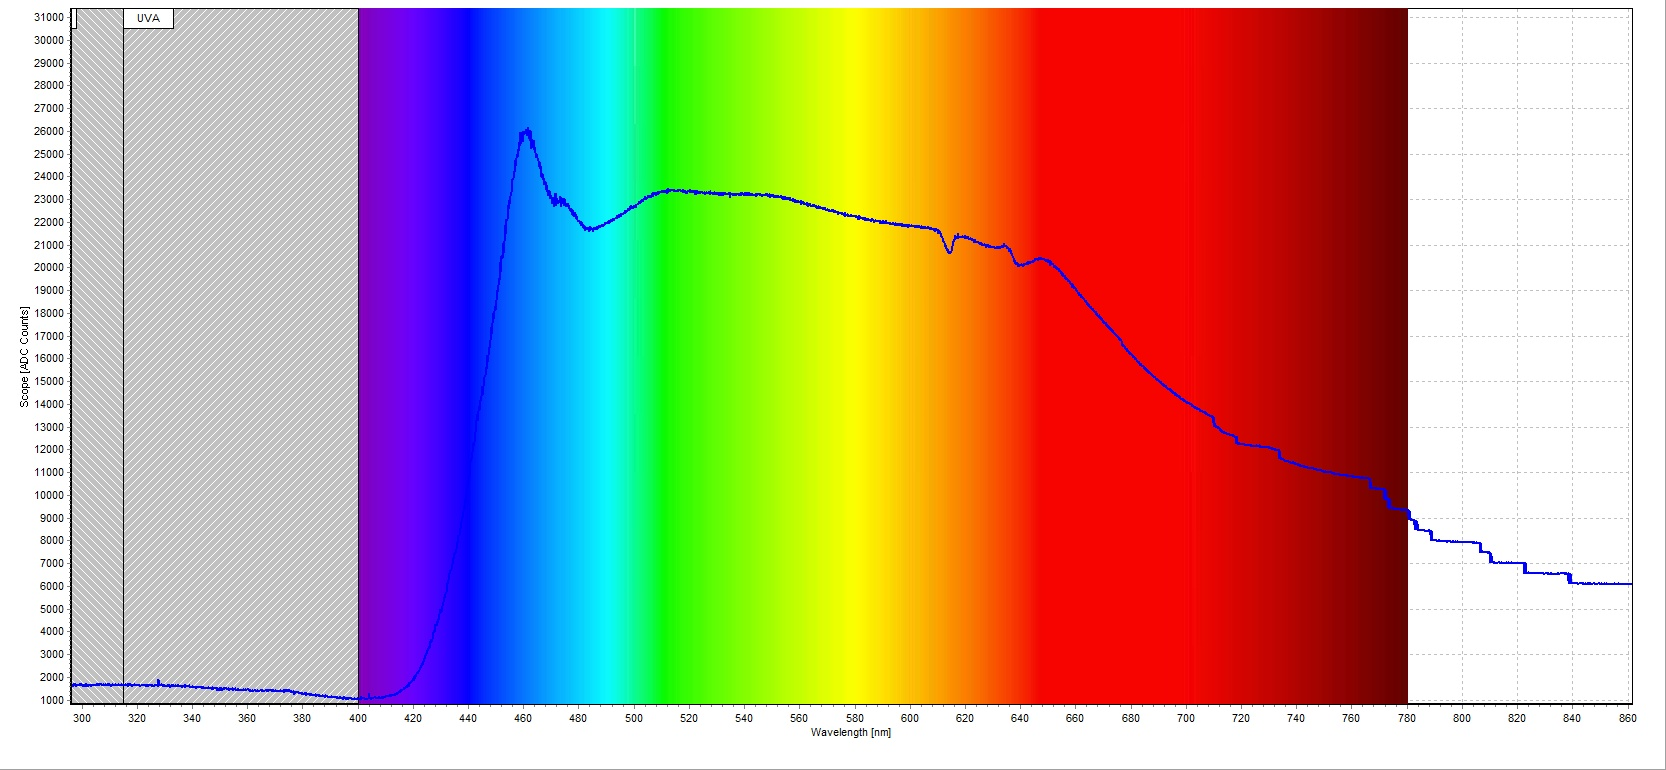
\includegraphics[width=0.9\textwidth]{Lab2_1Gra_A_phone2.jpg}
			\caption{手机闪光灯的发光光谱}
			\label{fig:figA8}
		\end{figure}
		
		\clearpage
		\item Beer定律验证
		
		验证Beer定律,我测量了一系列浓度的高锰酸钾溶液的光吸收曲线,最终结果如\cref{fig:figA9}所示,更进一步的解读与分析见\textbf{数据分析}部分。
		
		\begin{figure}[htbp]
			\centering
			\subfloat[]{
				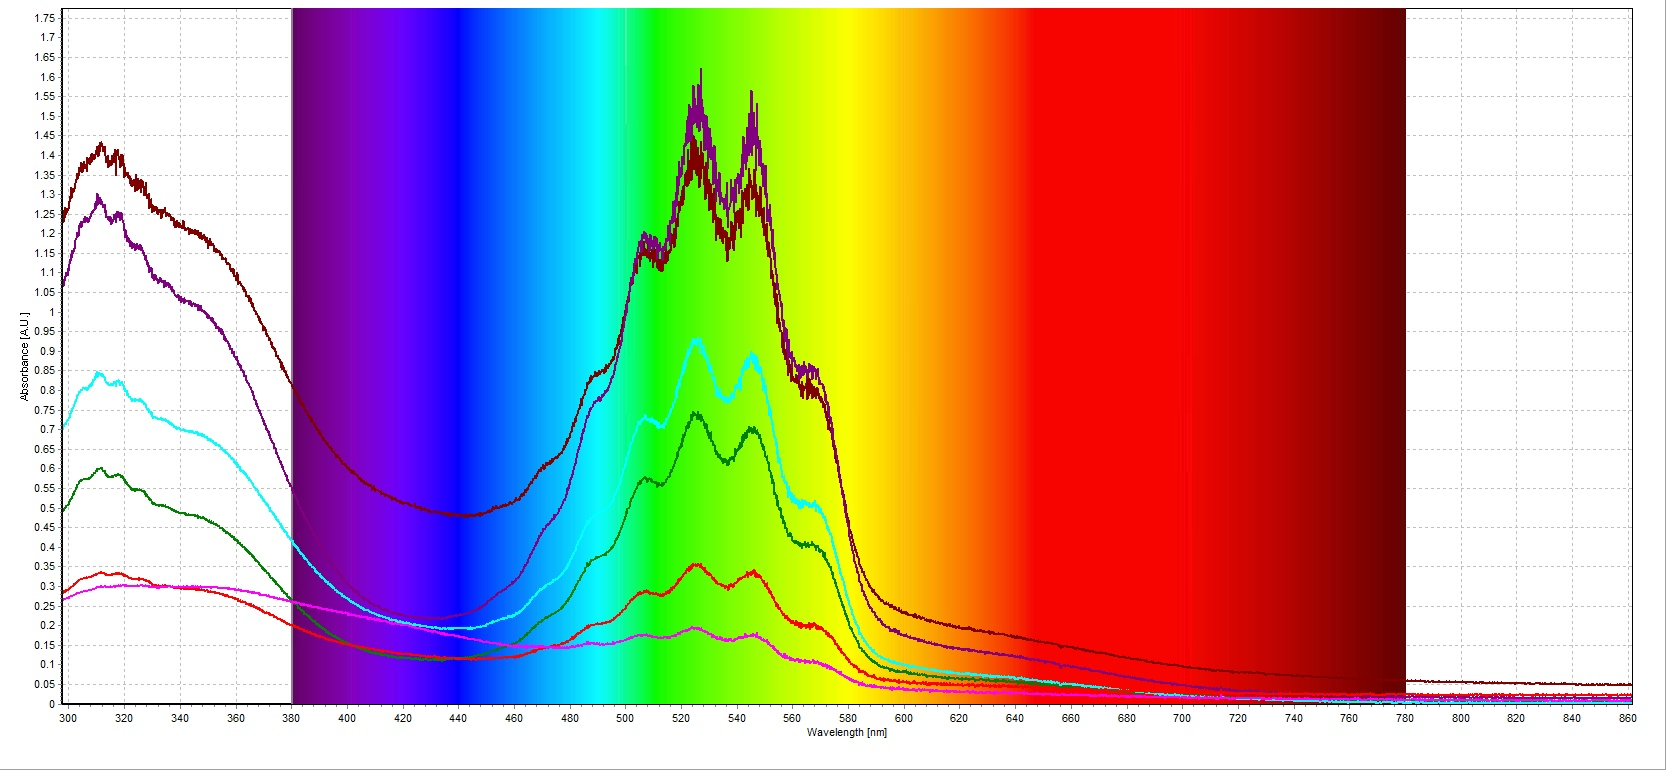
\includegraphics[width=0.45\textwidth]{Lab2_1Gra_A_KMnO4all1.jpg}
			}
			\subfloat[]{
				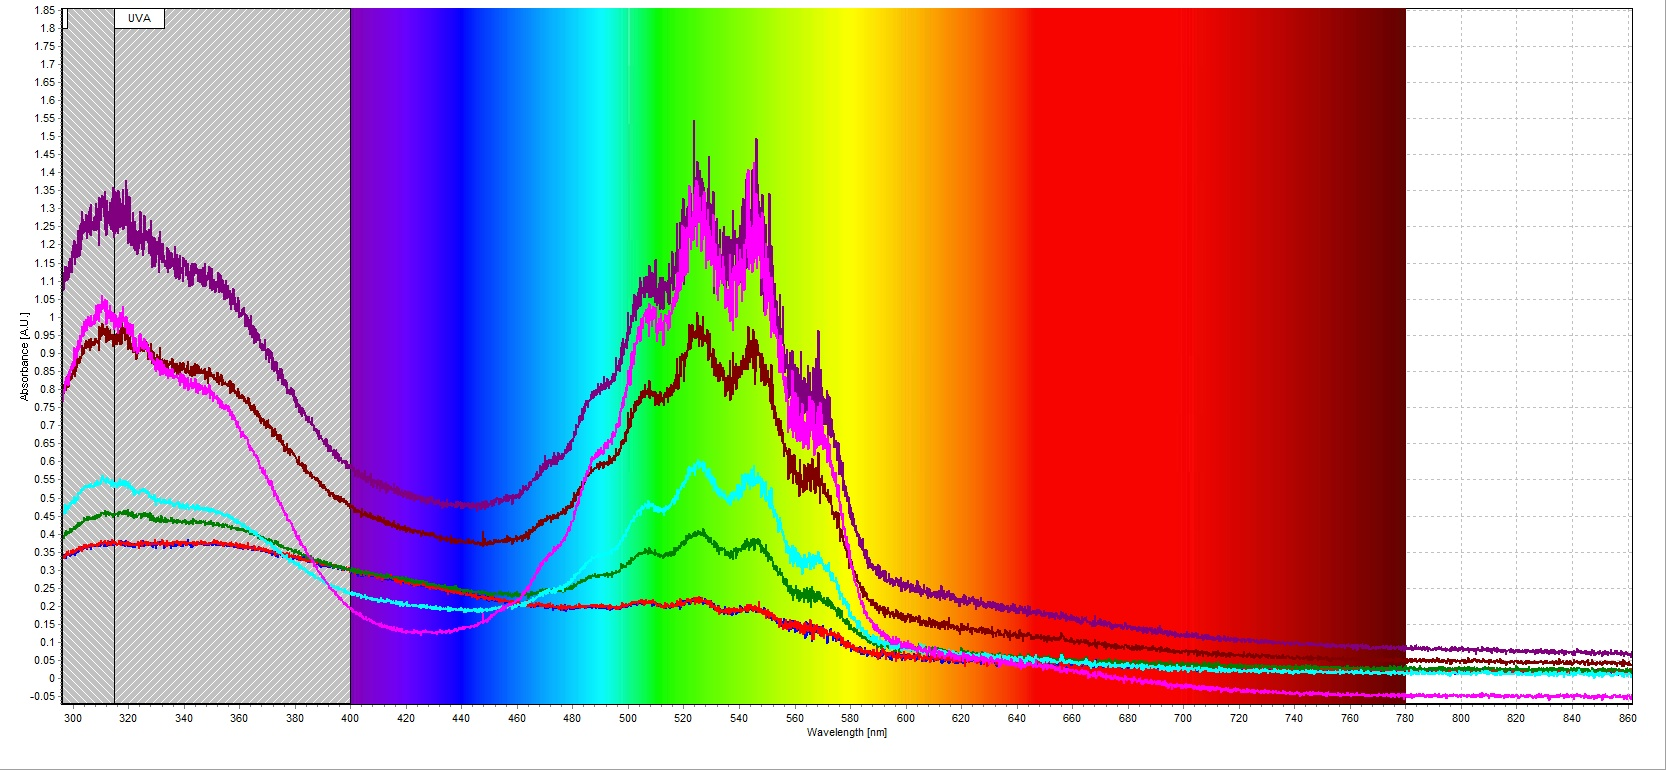
\includegraphics[width=0.45\textwidth]{Lab2_1Gra_A_KMnO4all2.jpg}
			}
			\caption{Beer定律验证}
			\label{fig:figA9}			
		\end{figure}
		
		\item Lambert定律验证
		
		验证Lambert定律,我测量了厚度增加薄片的光透射曲线,最终结果如\cref{fig:figA10}所示,更进一步的解读与分析见\textbf{数据分析}部分。
		
		\begin{figure}[htbp]
			\centering
			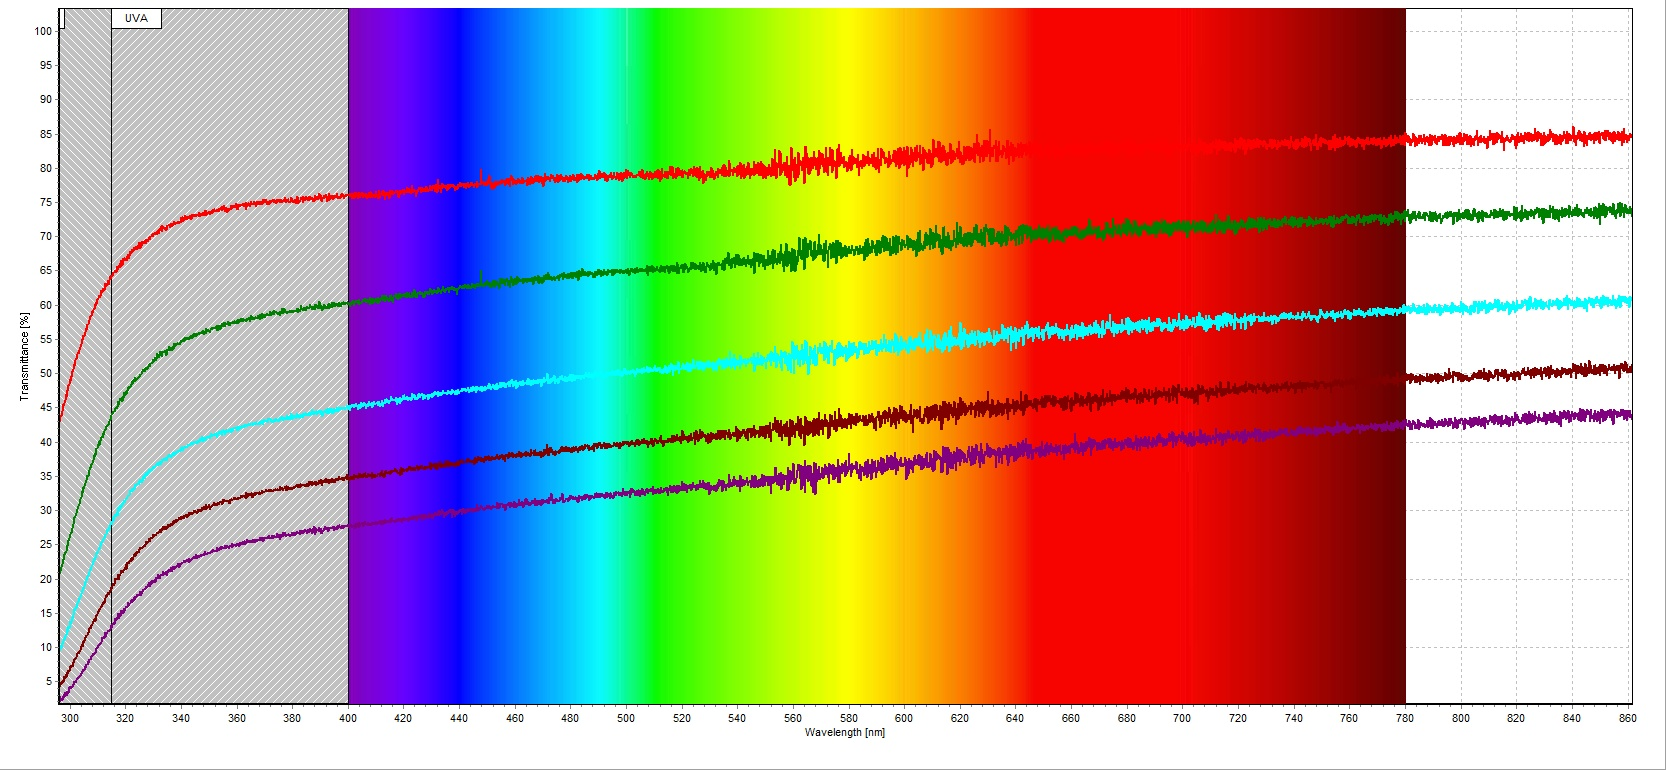
\includegraphics[width=0.9\textwidth]{Lab2_1Gra_A_plateall.jpg}
			\caption{Lambert定律验证}
			\label{fig:figA10}
		\end{figure}
		
	\end{enumerate}
	
	% ---
	
	% 原始数据
	\clearpage
	\subsection{原始数据记录}
	(实验记录本上的)原始数据签字见\cref{fig:figAD1}(签字)。
	
	\begin{figure}[htbp]
		\centering
		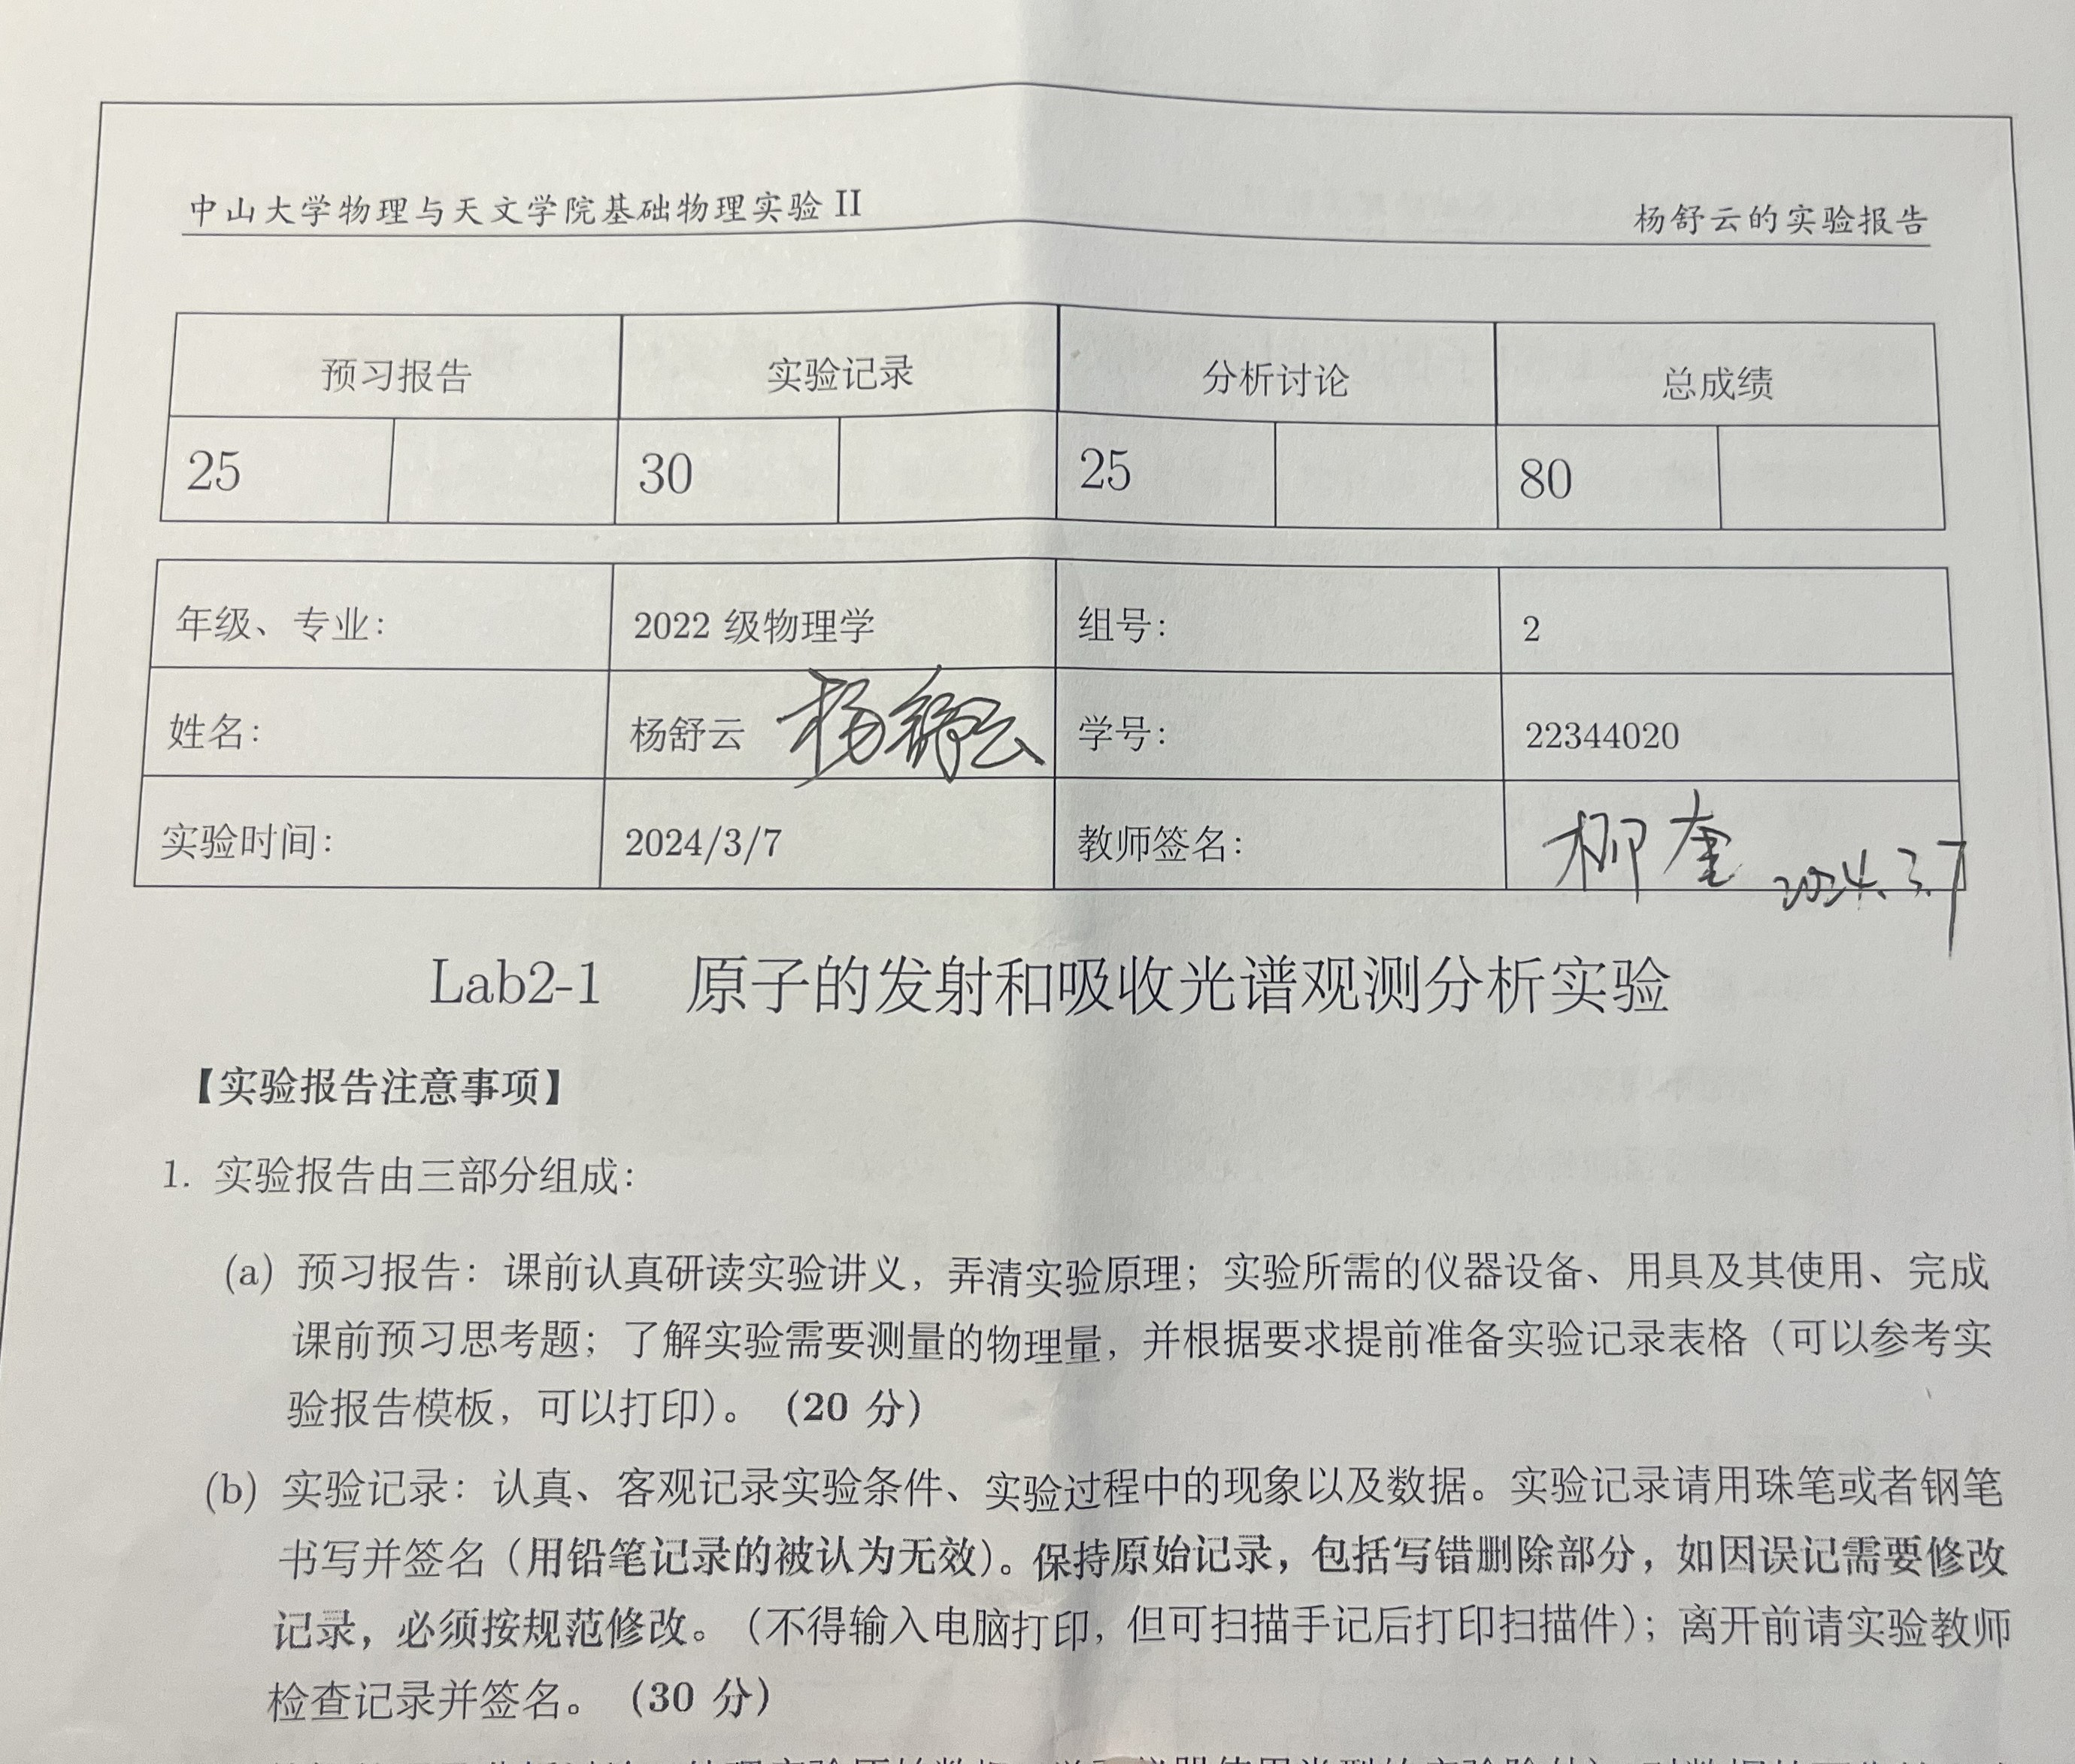
\includegraphics[width=0.7\textwidth]{Lab2_1GraAD1.jpg}
		\caption{原始数据签字}
		\label{fig:figAD1}
	\end{figure}
	
	%实验台桌面整理见%\textbf{附件}部分(\cref{})。
	
	%其它原始数据见%\cref{}。
	% ---
	
	% 问题记录
	\subsection{实验过程中遇到的问题记录}
	\begin{enumerate}
		\item 可能是实验设备的原因,实验所测得数据有着不小的噪声;因此,我用Python语言编写了滤波器代码来降低噪声的影响,详见\textbf{数据分析}部分。
		\item 钠灯光谱测量效果不好而且难以分析。
	\end{enumerate}
	% ---
	
	
	
	% 分析与讨论	
	\clearpage
	
	% 顶栏
	\begin{table}
		\renewcommand\arraystretch{1.7}
		\begin{tabularx}{\textwidth}{|X|X|X|X|}
			\hline
			专业:& 物理学 &年级:& 2022级\\
			\hline
			姓名: & 杨舒云 & 学号:& 22344020\\
			\hline
			日期:& 2023/3/7 & 评分:& \\
			\hline
		\end{tabularx}
	\end{table}
	% ---
	
	% 小标题
	\section{Lab2-1 原子的发射和吸收光谱观测分析实验 \quad\heiti 分析与讨论}
	% ---
	
	% 数据处理
	\subsection{实验数据分析}
	
	%
	\subsubsection{钠灯光谱的谱线分析}
	\begin{enumerate}
		\item 测量结果与光谱图基本信息解读
		回顾\textbf{原理概述}部分所述钠原子光谱特点,
		钠原子光谱分四个线系:主线系np-3s(n=3,4,5,…),锐线系ns-3p(n=4,5,6,…),漫线系nd-3p(n=3,4,5,…),基线系nf-3d(n=4,5,6,…)。
		然后利用实验测得的数据分别得到钠黄双线图与300-550nm图(\cref{fig:fig7}和\cref{fig:fig8})。(杂峰的存在严重影响的钠谱线的定位,所以除了那些很强的钠谱线外,在不知道理论波长时是无法从图中确定哪些是钠的谱线,所以本人通过钠谱线的双线结构并参考了理论值在图中已经定出了钠的谱线。)
		
		\begin{figure}[htbp]
			\centering
			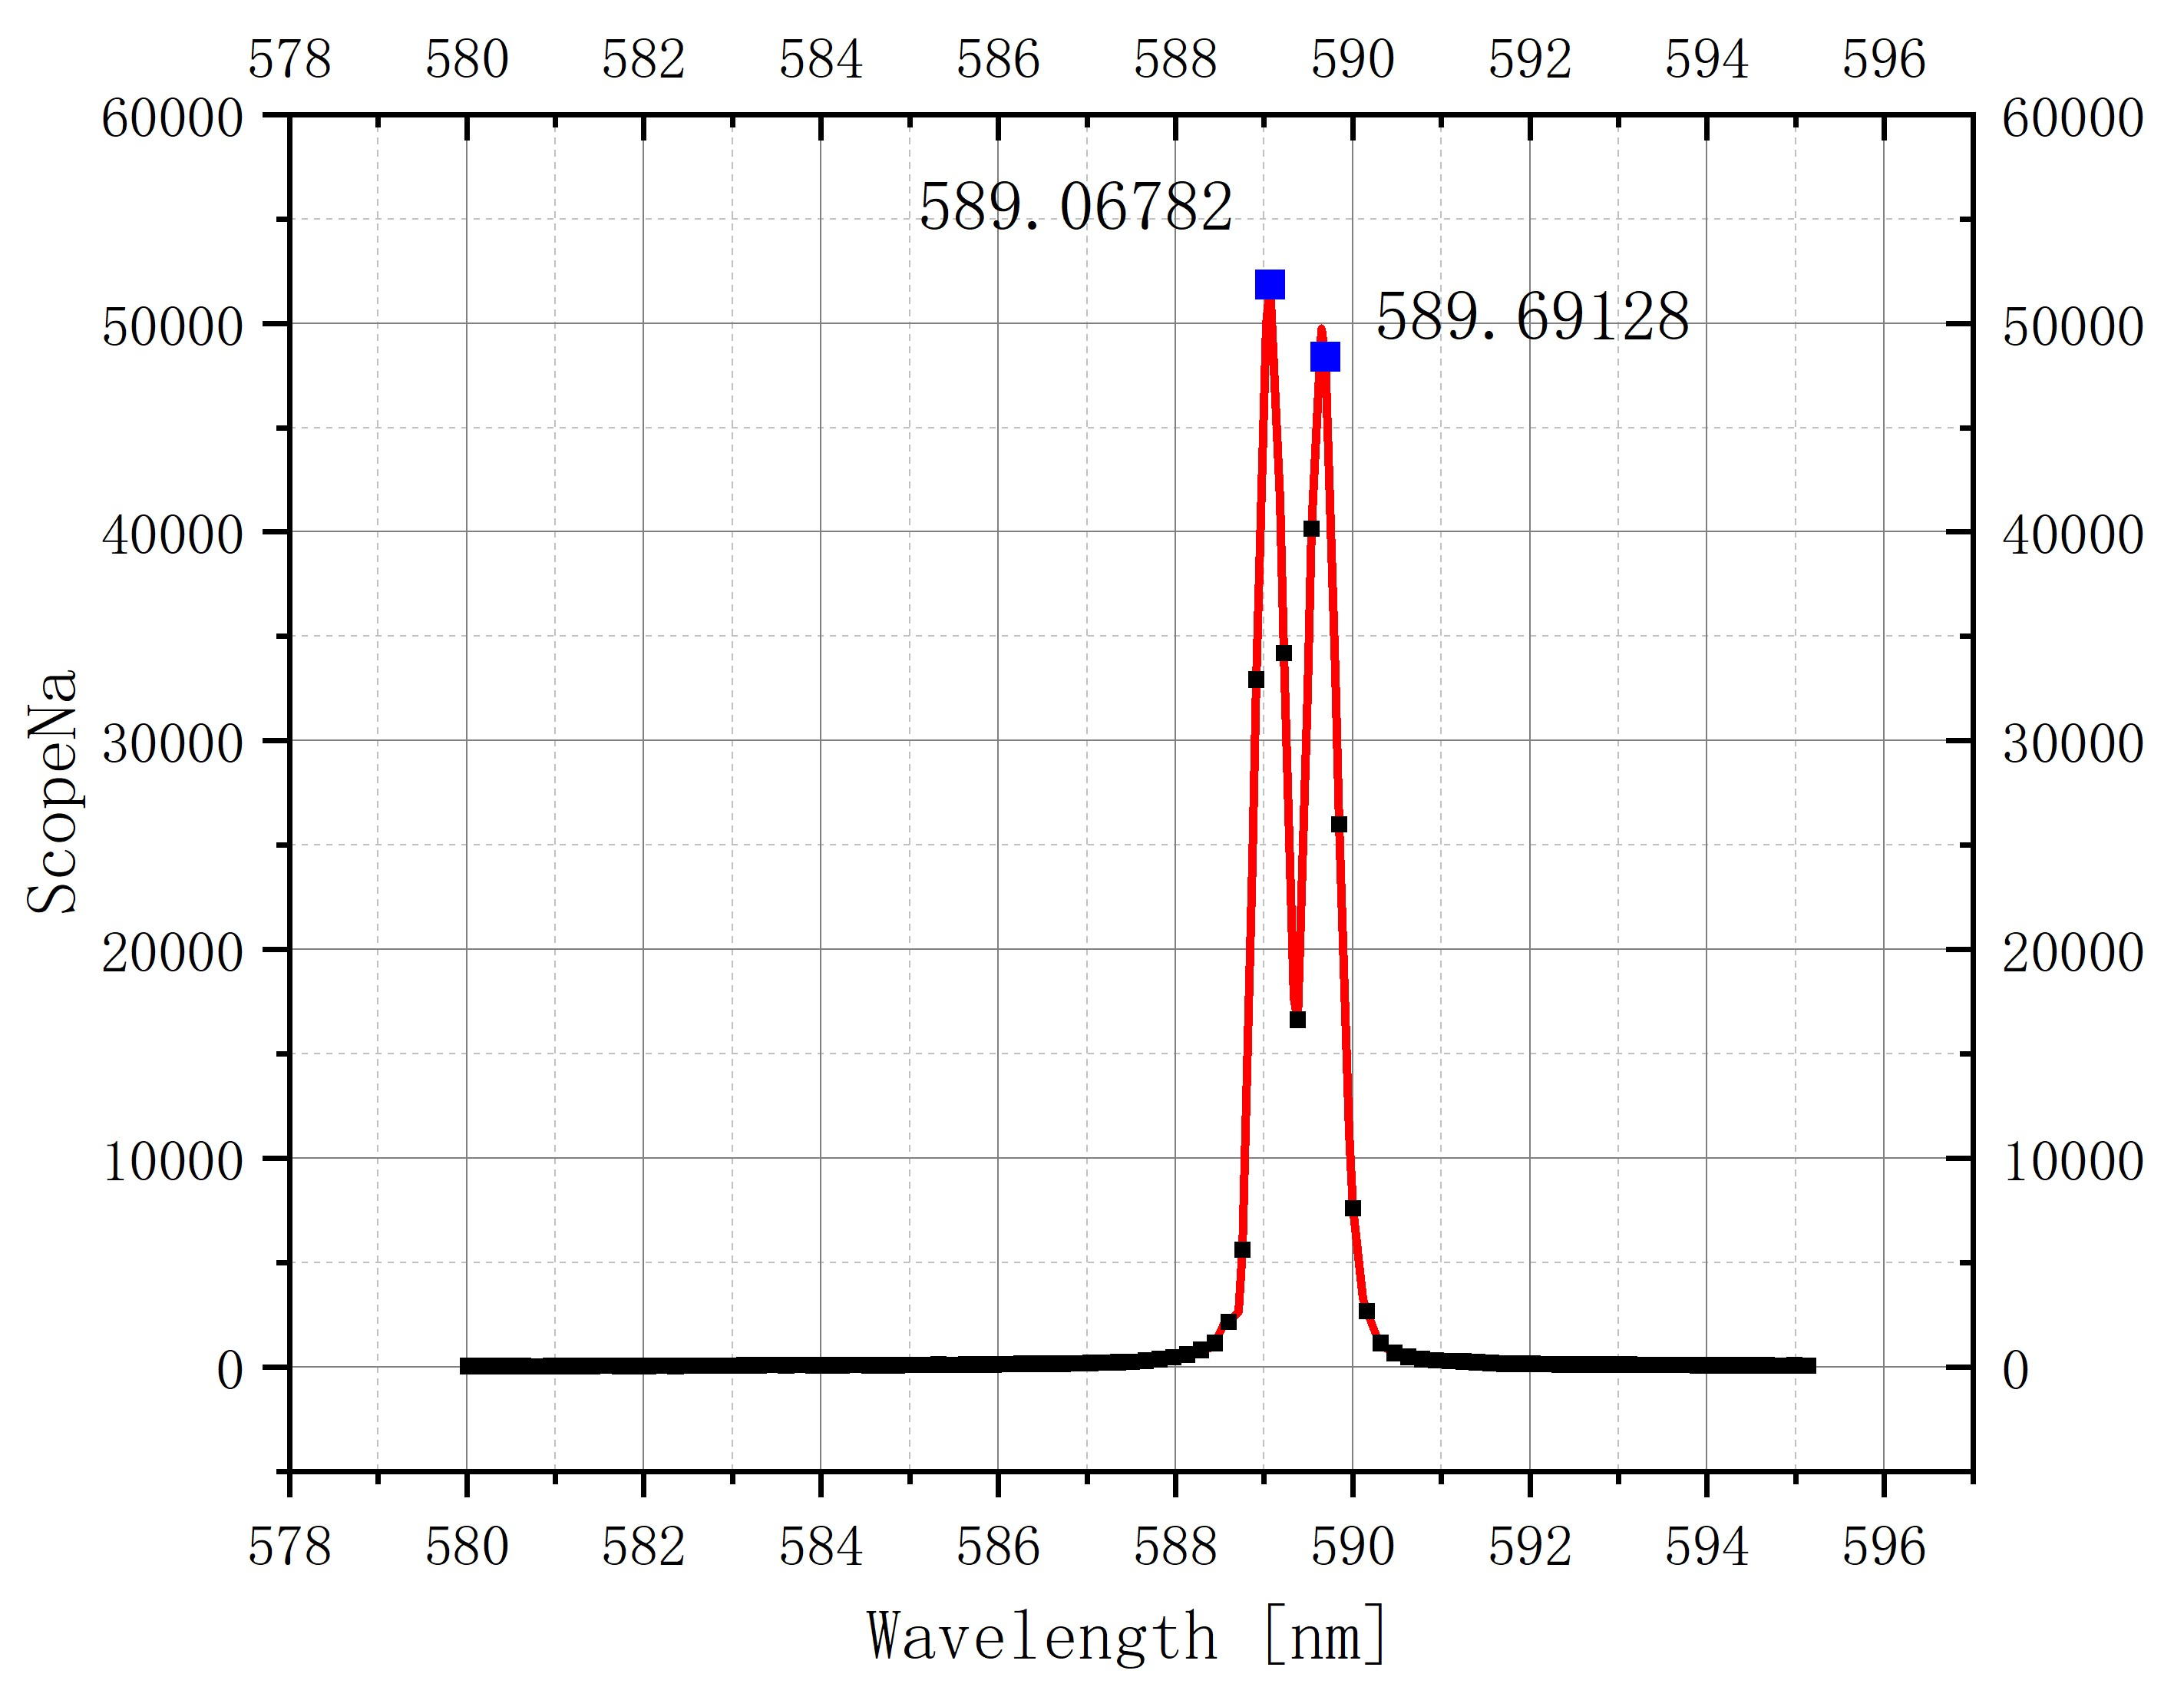
\includegraphics[width=0.7\textwidth]{Lab2_1Gra7.jpg}
			\caption{钠黄双线图}
			\label{fig:fig7}
		\end{figure}
		
		\begin{figure}[htbp]
			\centering
			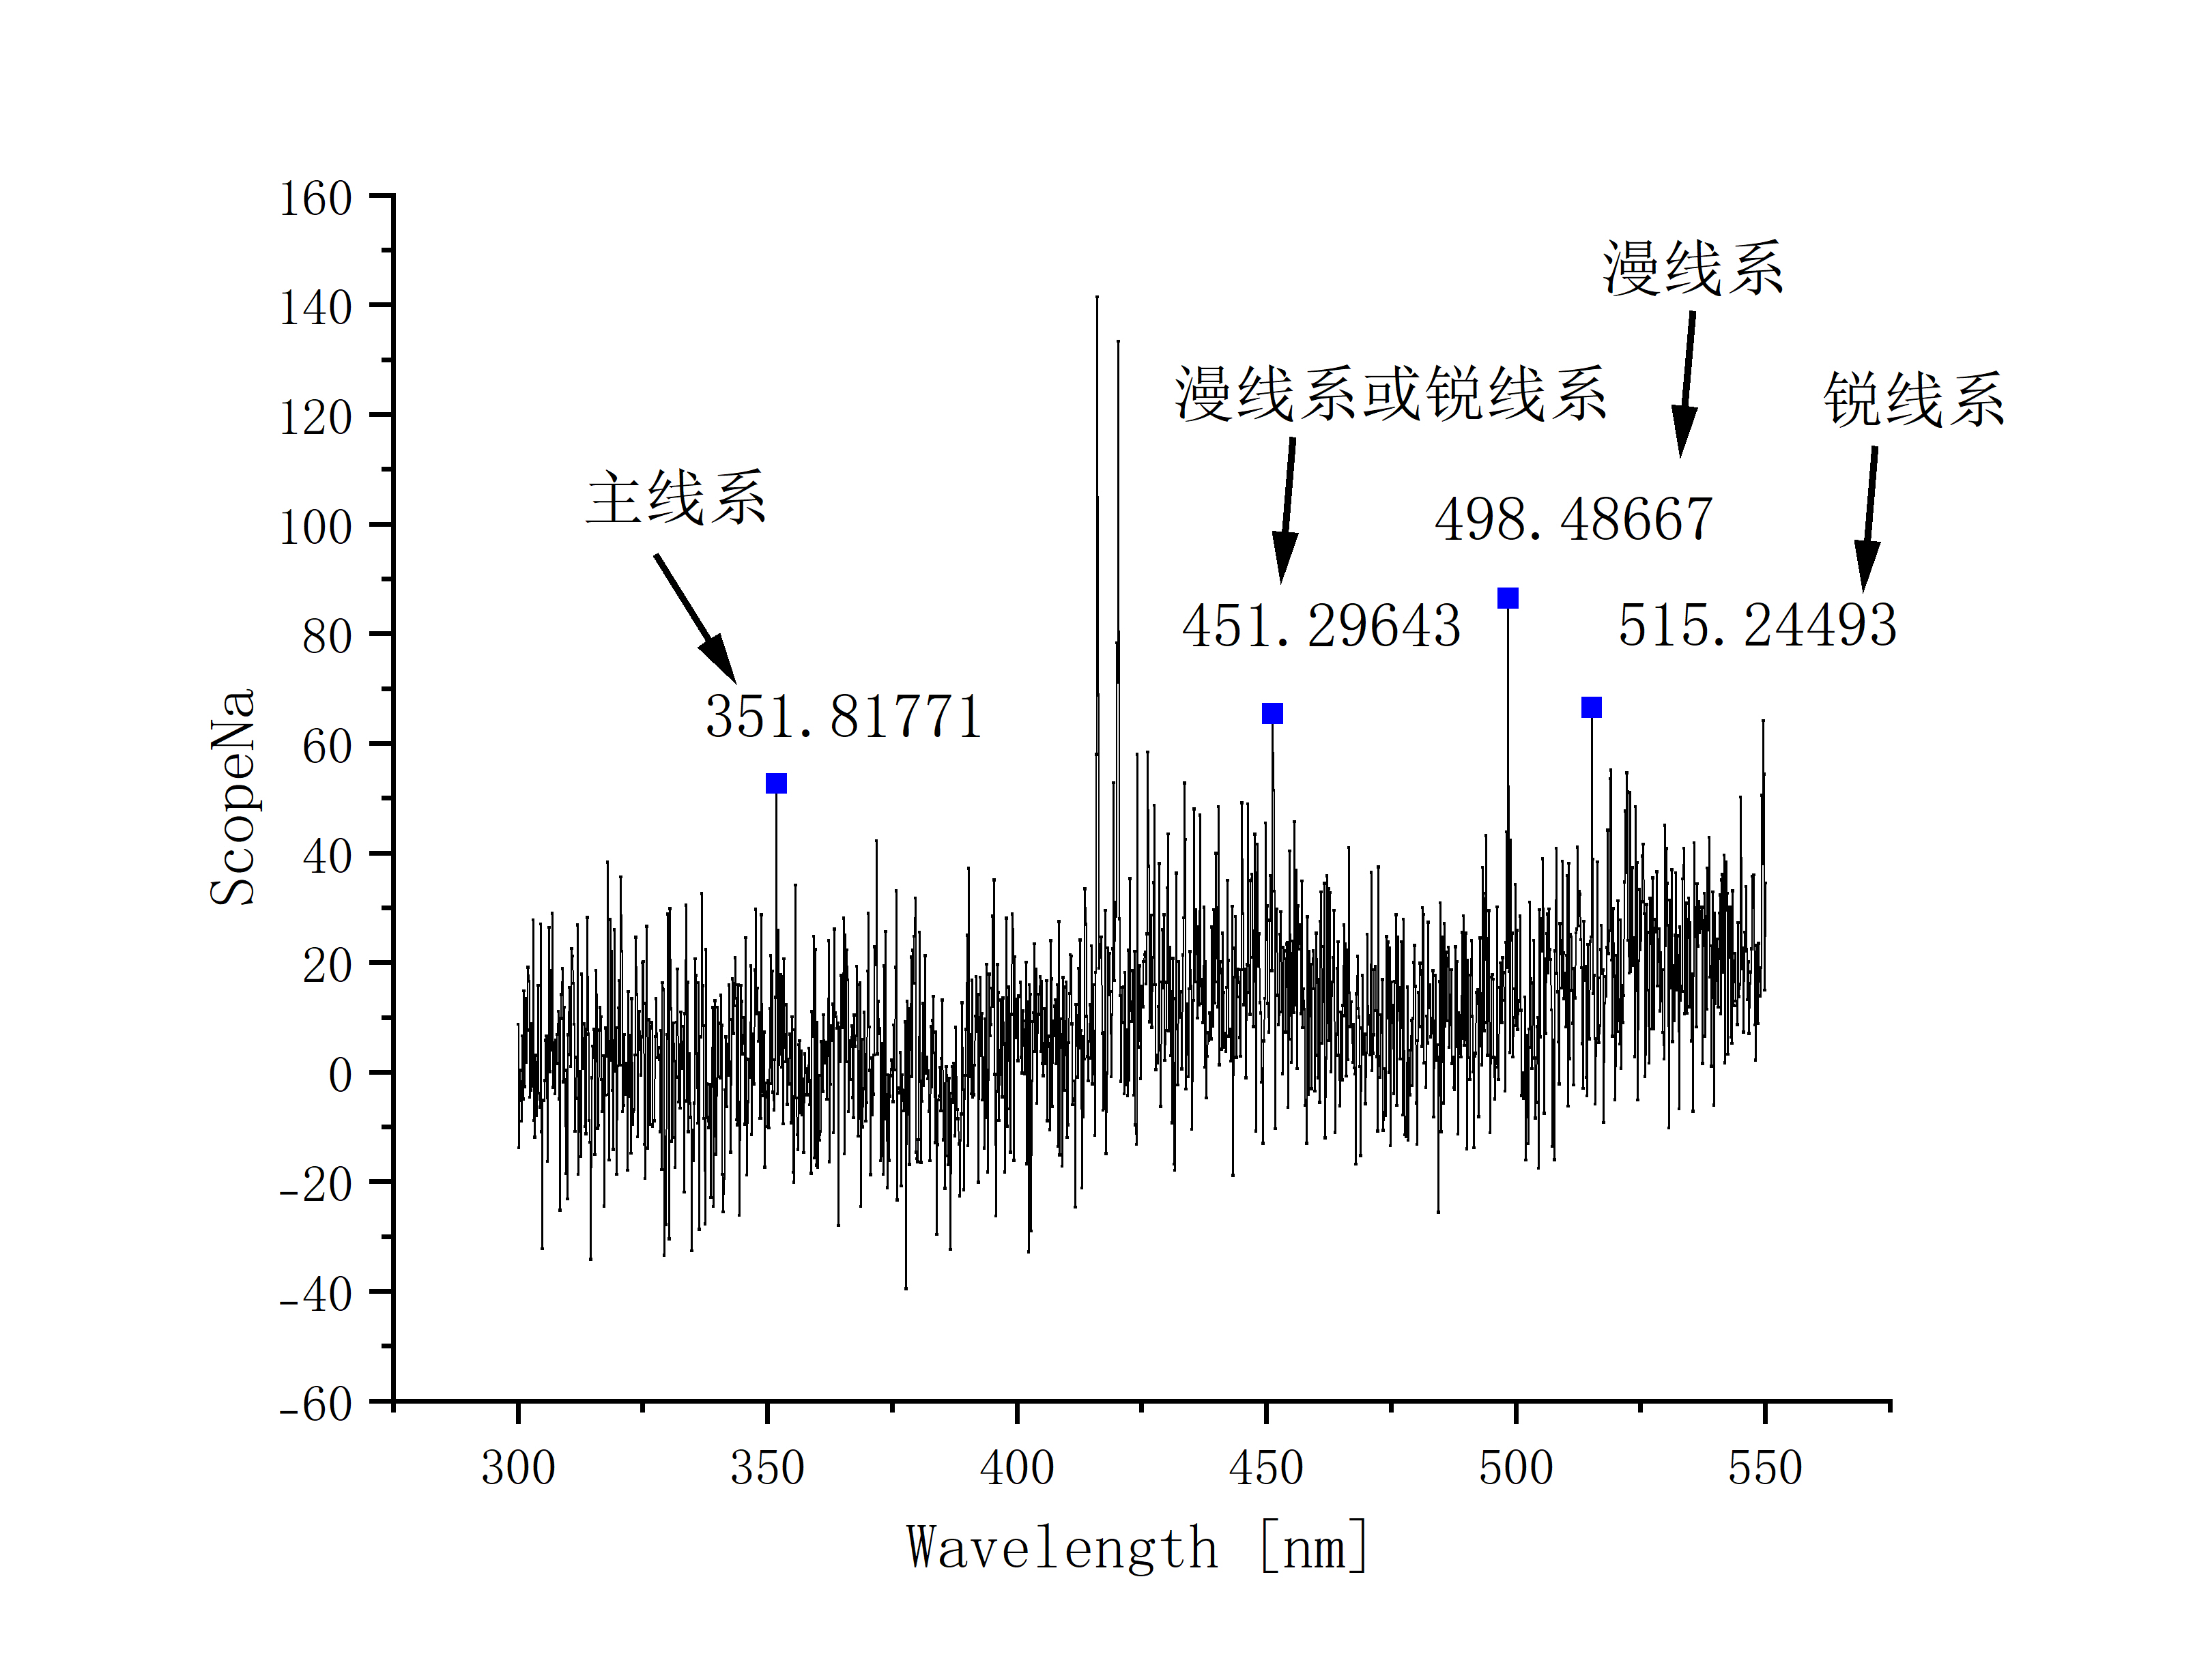
\includegraphics[width=0.6\textwidth]{Lab2_1Gra8.jpg}
			\caption{300~550nm图}
			\label{fig:fig8}
		\end{figure}
		
		\item 谱线数据处理与计算
		
		光谱分析的基础是碱金属原子的最外层只有一个价电子,而内层电子与原子核形成较为稳固的集团(原子实),价电子和原子实的相互作用会造成量子亏损。量子亏损会使得电子的实际能级低于没有外层电子影响时的理论能级。
		
		利用所得到的谱线数据(\cref{tab:tab1}),我们可以结合\textbf{原理概述}部分所提到的量子亏损做一些计算。
		
		利用谱线数据计算能级跃迁。钠原子的光谱跃迁可以表示为:
		\[
		\nu = \frac{1}{\lambda} = R_H \left( \frac{1}{(n_1 + \Delta_1)^2} - \frac{1}{(n_2 + \Delta_2)^2} \right)
		\]
		其中\( R_H \)是里德伯常数,\( n_1 \)和\( n_2 \)分别是初态和末态的主量子数,\( \Delta_1 \)和\( \Delta_2 \)是对应的量子亏损。
		
		据此可以计算一些非常有物理意义的物理量的值。
		
		\textbf{有效核电荷数}(\( Z^* \)):这个值反映了核对最外层电子的有效吸引力,与实际的核电荷不同,因为内层电子对核电荷有屏蔽效应。有效核电荷数对于理解原子的化学性质至关重要。
		
		\textbf{量子亏损}(\( \Delta \)):在碱金属原子如钠原子中,量子亏损描述了由于原子实的极化和轨道贯穿效应,使得价电子能级与理论预测存在偏差。对于不同的电子轨道(s、p、d等),量子亏损各不相同。量子亏损能够帮助我们理解和计算复杂原子系统的光谱特性。
		
		\textbf{谱线波长与能级跃迁的关系}:通过分析光谱中的谱线波长,我们可以确定电子从一个能级跃迁到另一个能级时释放或吸收的光子的能量。这直接关系到原子的能级图,是量子力学中的基础概念。
		
		我们已知主线系的量子亏损为\( \Delta_p = 0.89 \)、漫线系的量子亏损为\( \Delta_d = 0.01 \),锐线系的量子亏损为\( \Delta_s = 1.35 \)。使用这些值,我们可以计算对应的能级差。
		
		钠双黄线的两条谱线分别对应于波长 589.07 nm 和 589.69 nm 的光子。通过计算得知,它们的能量分别约为 2.105 eV 和 2.103 eV。由于量子亏损的影响,我们计算的跃迁能量非常接近,但由于它们处在相同的能级跃迁(主线系的 3P 到 3S 跃迁),理论上它们应该是相同的。这个非常小的差异(约 \(8.71 \times 10^{-8}\) eV)来自于精细结构的效应,这也正是量子亏损的物理意义所在。它揭示了原子内部复杂相互作用的微妙之处,包括电子自旋和轨道角动量的耦合。
		
		\begin{table}[ht]
			\centering
			\begin{tabular}{|c|c|c|}
				\hline
				Na双黄测量值/nm & 589.1 & 589.7 \\
				\hline
				Na双黄理论值/nm & 589.0 & 589.6 \\
				\hline
			\end{tabular}
			\caption{Na双黄测量值与理论值}
			\label{tab:tab1}
		\end{table}		
		
		\item 关于杂峰
		
		已知钠灯中会填充惰性气体,因此考虑杂峰\textbf{可能}是惰性气体受激跃迁辐射光谱。
		
		利用实验室软件读出各小峰波长值,再查询资料找到各种惰性气体的光谱,发现氩原子光谱与小峰对应的很好,说明实验中使用的钠灯填充的是氩气,\textbf{猜测}扫描出的谱线中的杂质峰是氩原子受激跃迁发射的光谱。
		
		\begin{figure}[htbp]
			\centering
			\subfloat[]{
				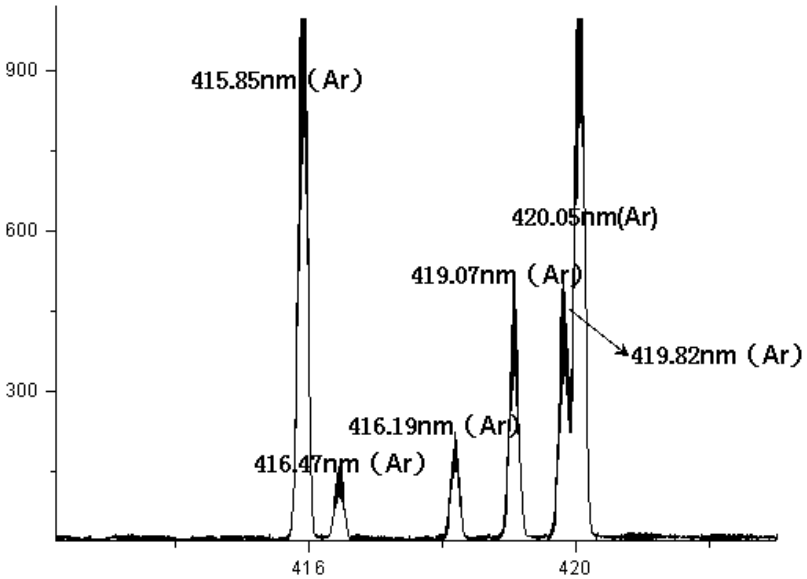
\includegraphics[width=0.4\textwidth]{Lab2_1Gra9.png}
			}
			\subfloat[]{
				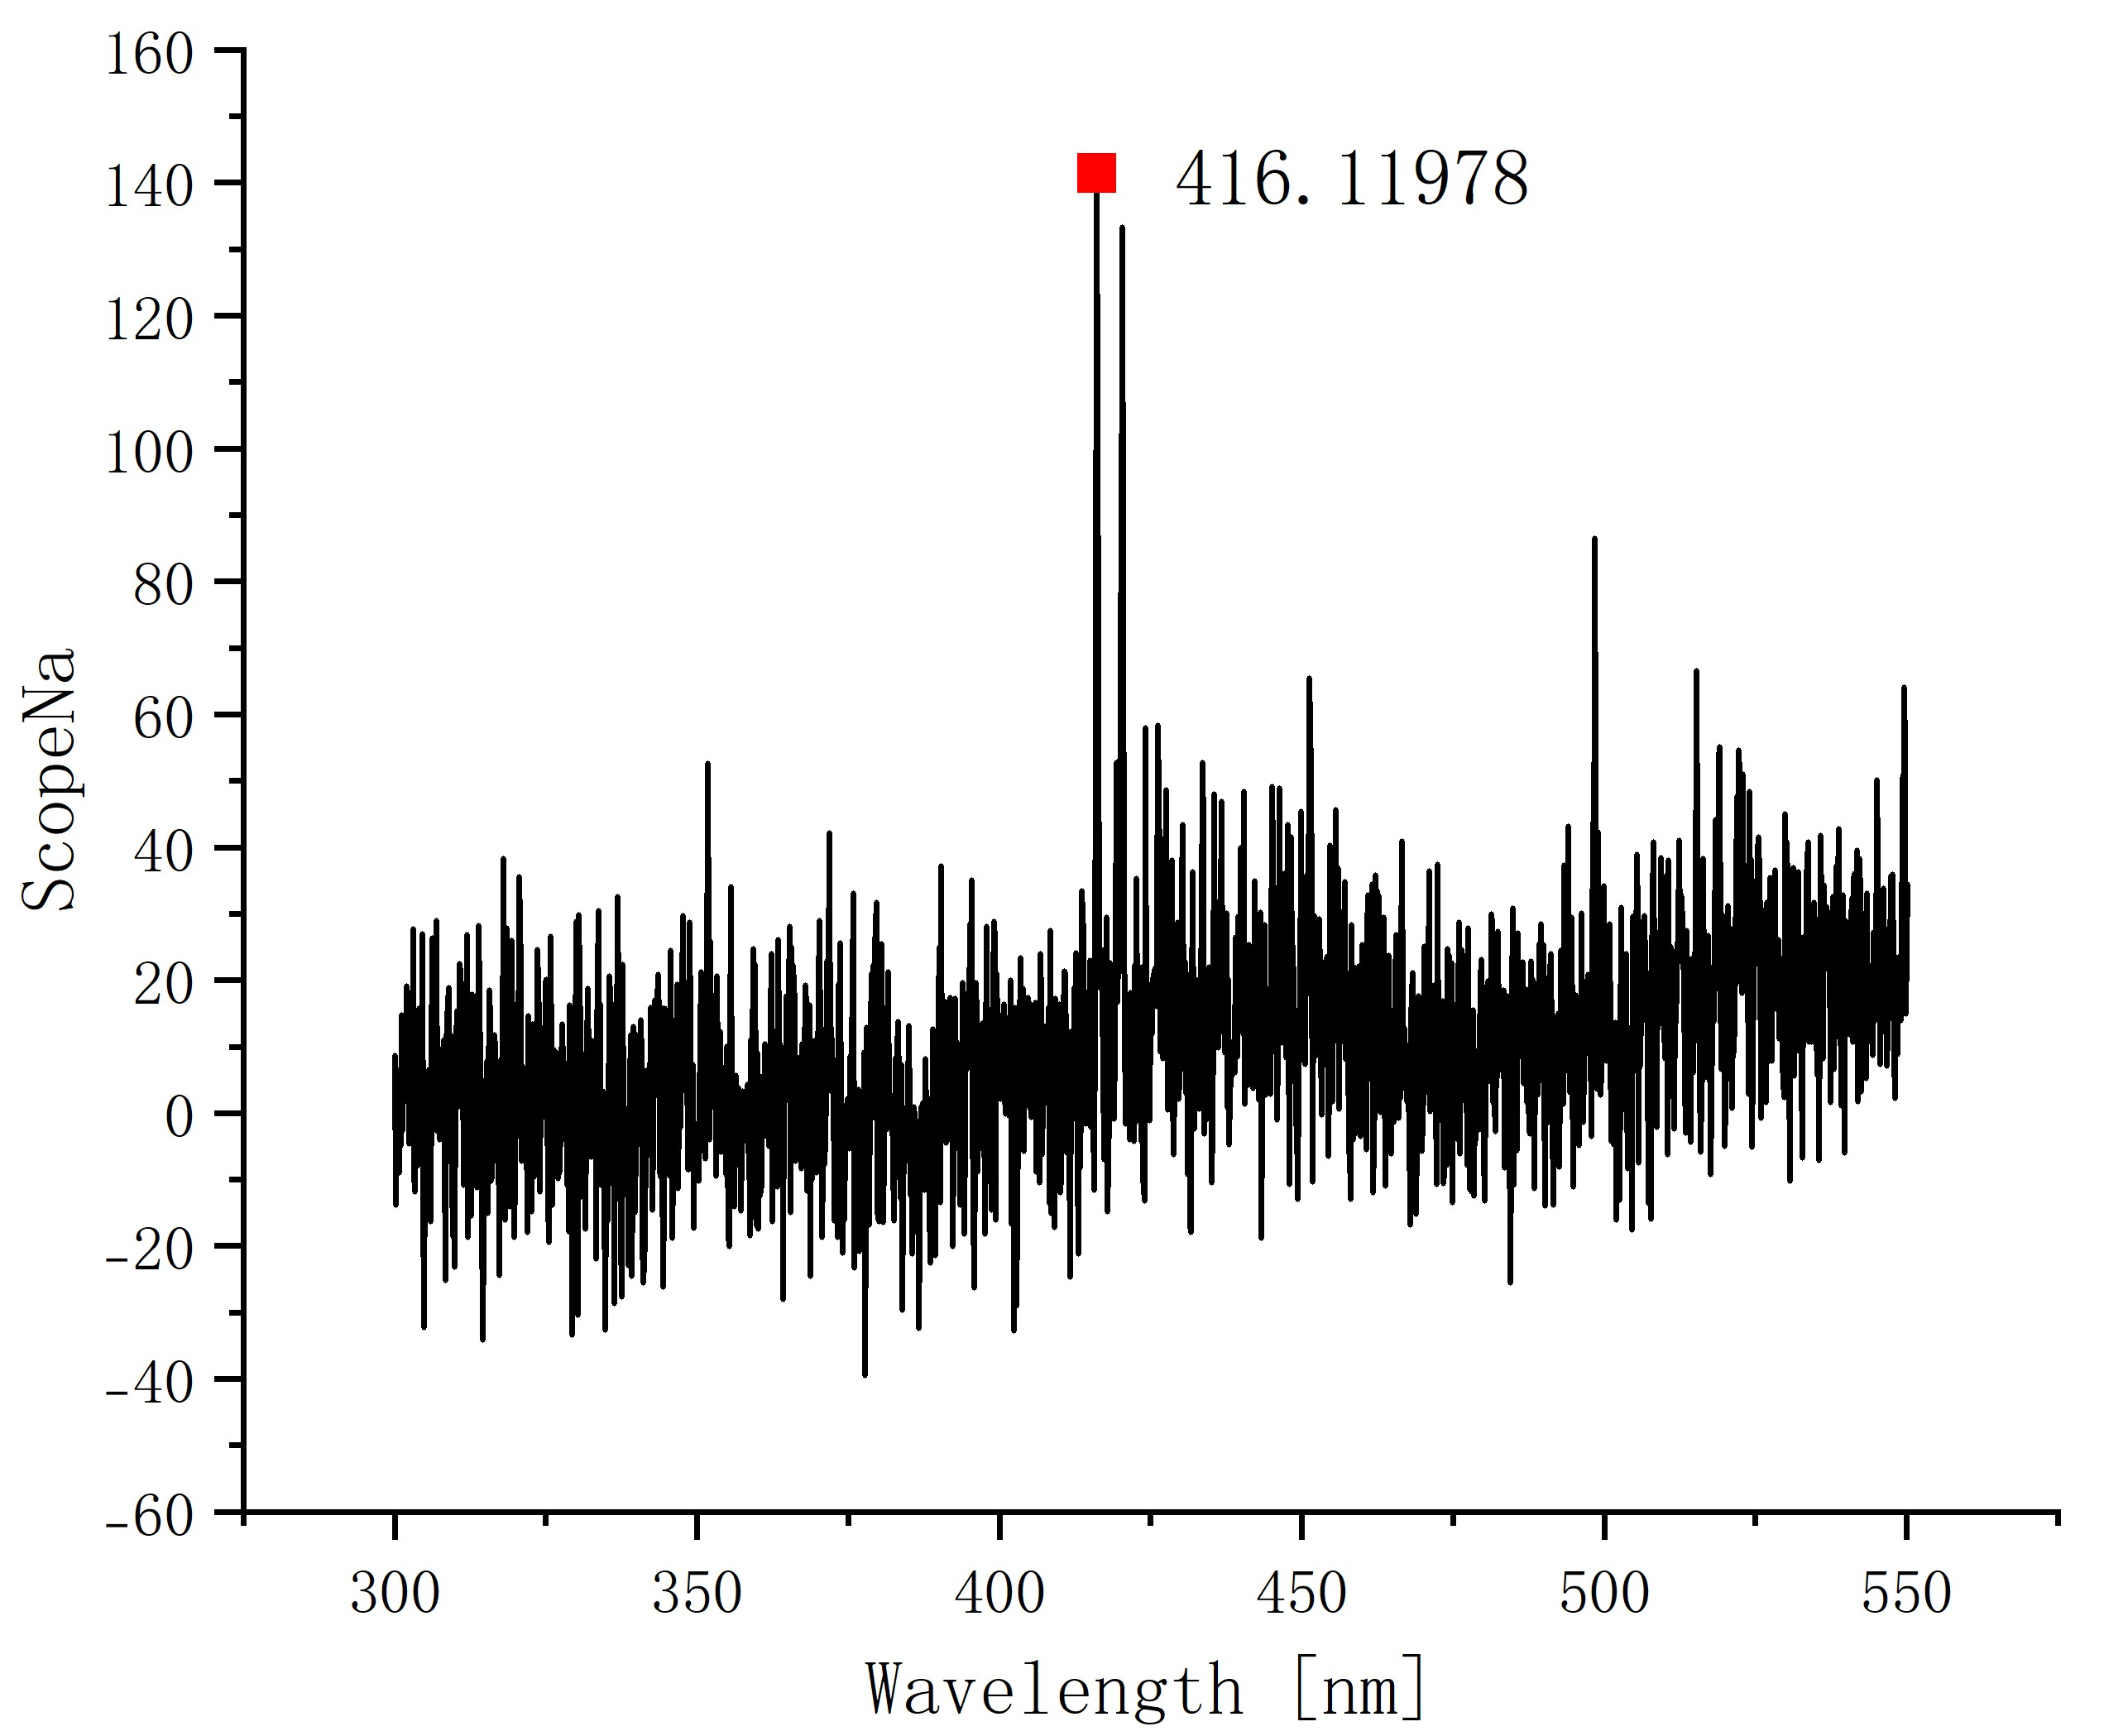
\includegraphics[width=0.35\textwidth]{Lab2_1Gra10.jpg}
			}
			\caption{关于杂峰}
			\label{fig:fig9}			
		\end{figure}
		
		事实上,对比两\cref{fig:fig9}可知,上述猜想在一定程度上符合。
		
	\end{enumerate}
	
	\subsubsection{汞灯光谱的谱线分析}
	关于汞灯光谱的光谱分析,这里主要判断所测得的光谱与实验“光栅常数及光波波长的测量”中所得到的汞灯谱线的差异,以此比较测量的精度。
	
	\textbf{查询“光栅常数及光波波长的测量”实验报告的原理概述部分,得到标准值:}
	
	\begin{center}
		\begin{tabular}{|c|c|}
			\hline
			波长 (nm) & 颜色 \\
			\hline
			184.5 & 紫外线 \\
			253.7 & 紫外线 \\
			365.4 & 紫外线 \\
			404.7 & 紫色 \\
			435.8 & 蓝色 \\
			546.1 & 绿色 \\
			578.2 & 黄色 \\
			1014 & 红外线 \\
			\hline
		\end{tabular}
	\end{center}
	
	\textbf{在实验“光栅常数及光波波长的测量”中,我们得到:}
	
	紫色取-1级与3级结果平均值$\bar{\lambda}(purple)=404.8nm$,相对误差0.02\%。
	
	蓝色取2级测量结果$\lambda(blue)=435.5nm$,相对误差-0.07\%。
	
	绿色取2级测量结果$\lambda(green)=545.4nm$,相对误差-0.12\%。
	
	黄色取各级结果平均值$\bar{\lambda}(yellow)=578.6nm$,相对误差0.06\%。
	
	\textbf{本实验中,我们得到如\cref{fig:fig11}所示数据:}
	
	\begin{figure}[htbp]
		\centering
		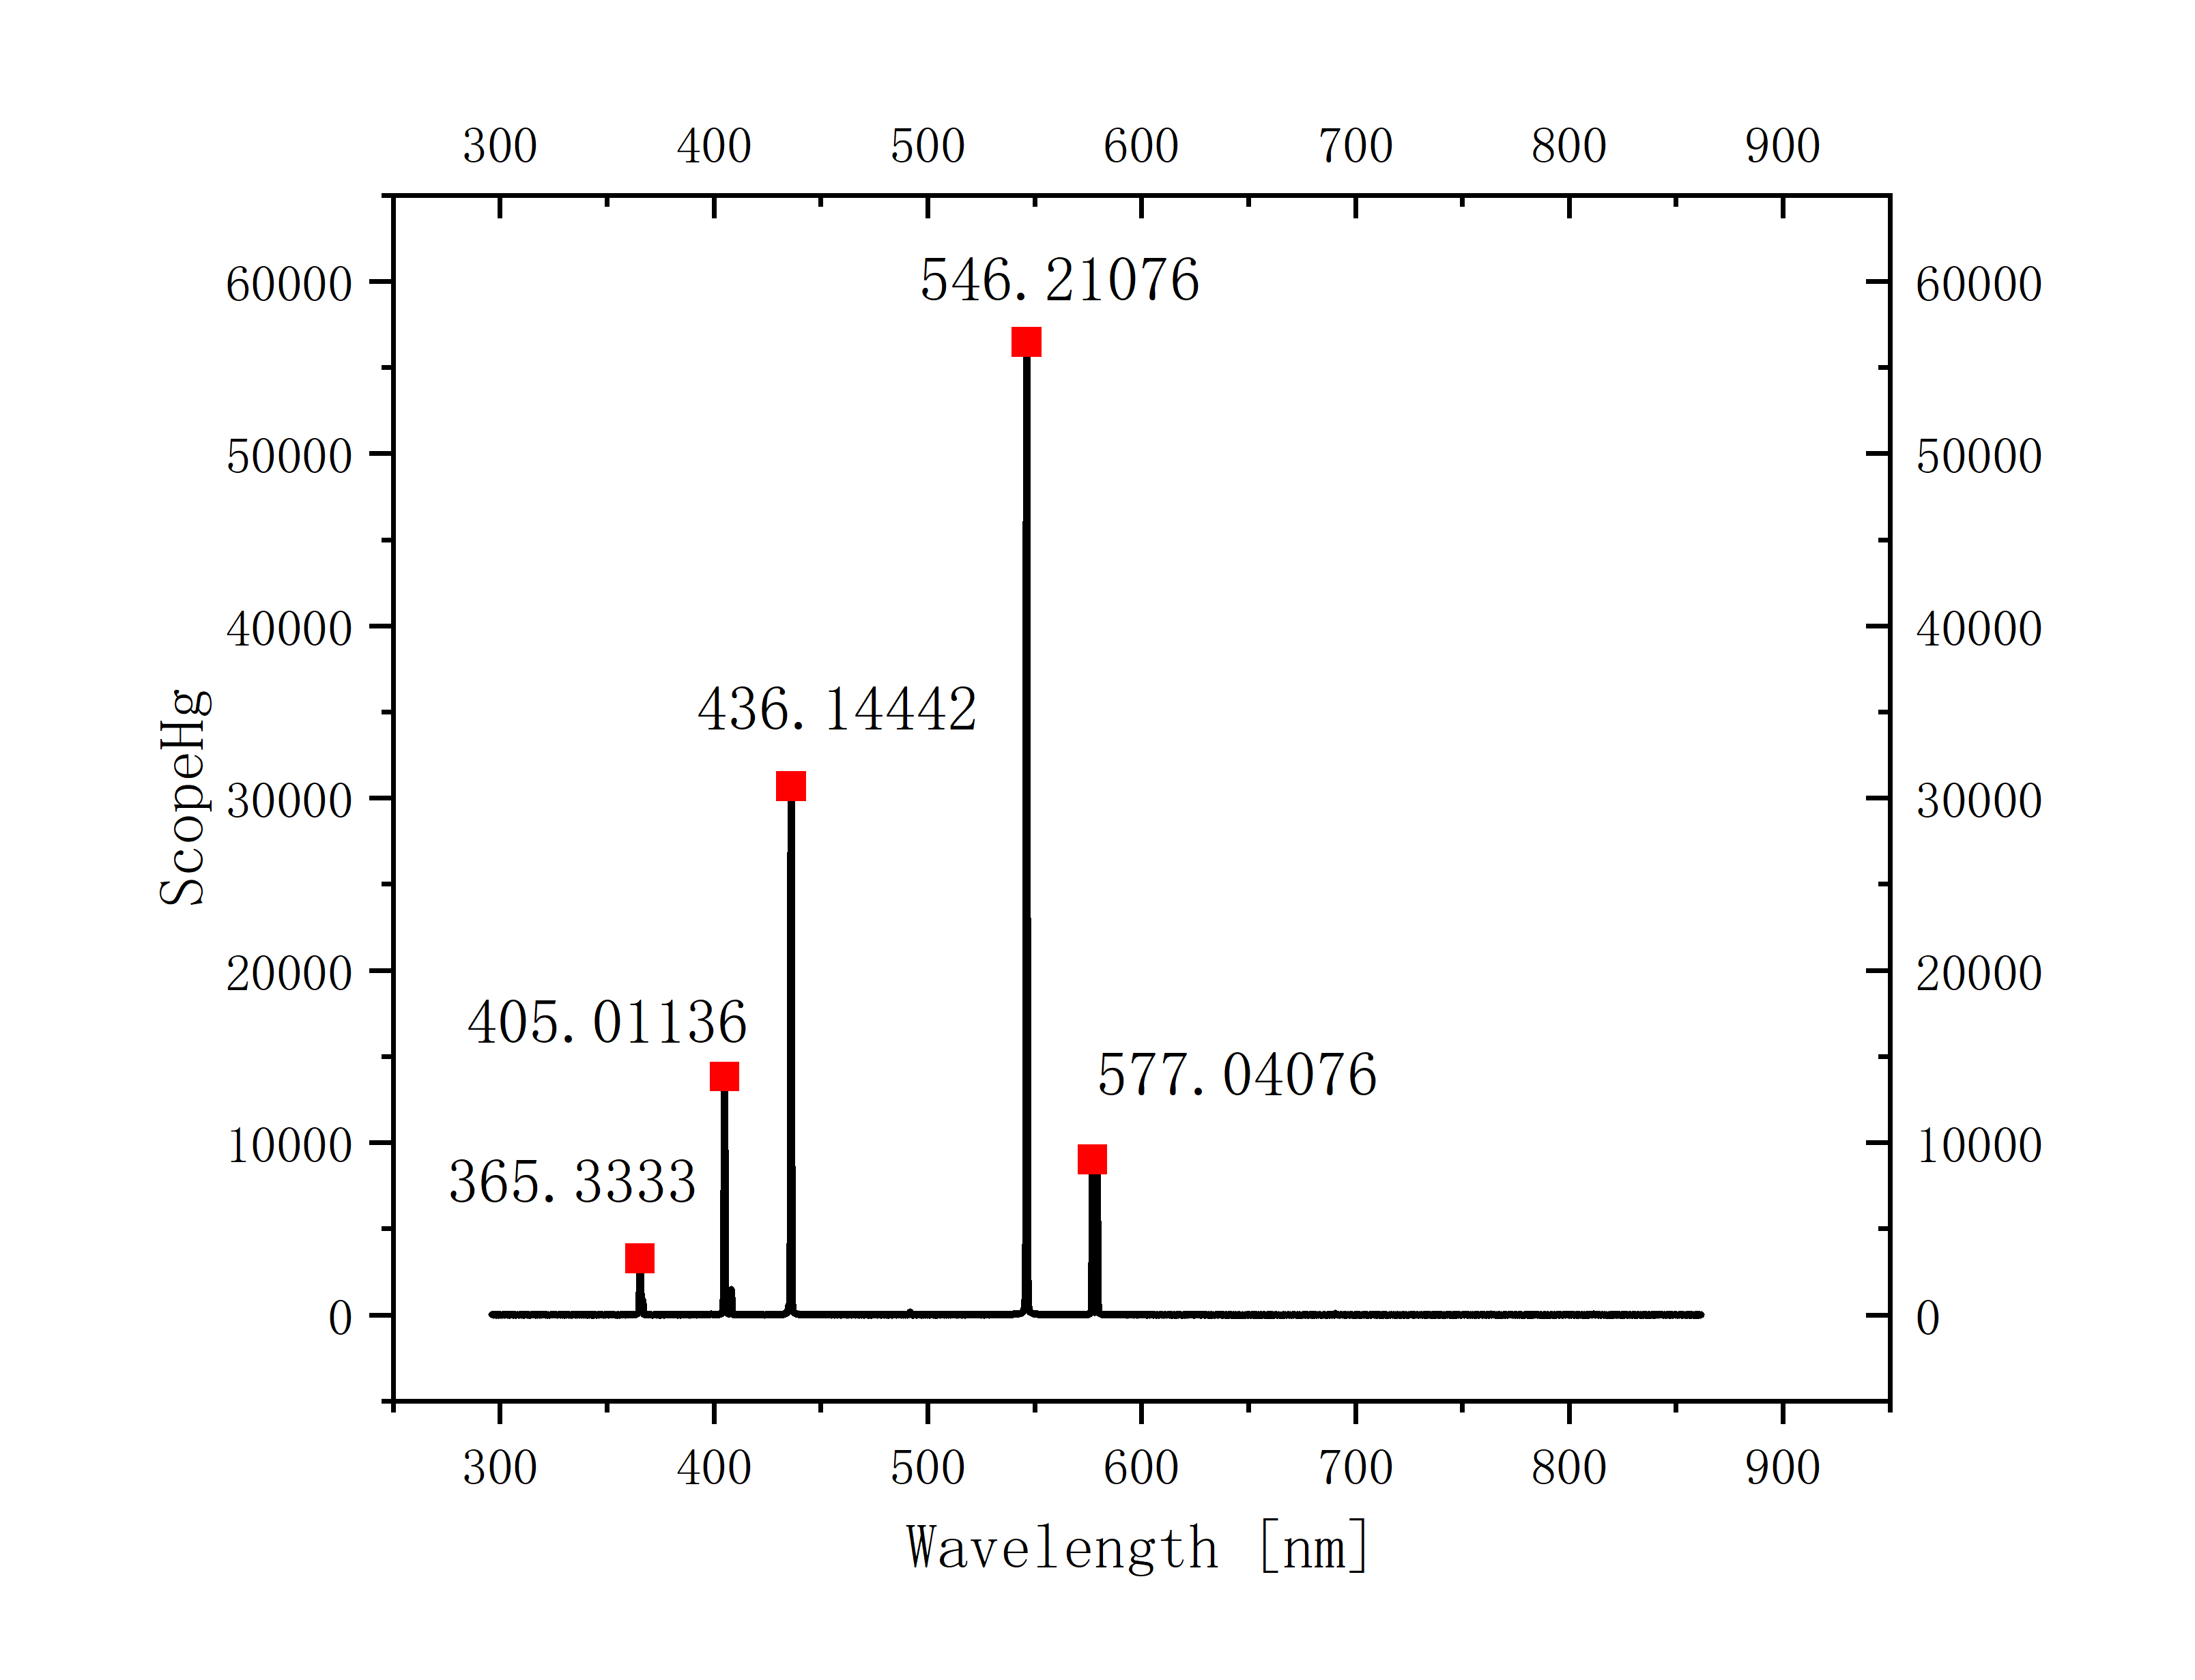
\includegraphics[width=0.7\textwidth]{Lab2_1Gra11.jpg}
		\caption{汞灯特征谱线对应波长示意图}
		\label{fig:fig11}
	\end{figure}
	
	对比可以发现,对于汞灯的特征谱线的测定是比较准确的。
	
	%
	\subsubsection{电灯(手机闪光灯)、手机屏幕光谱分析}
	\begin{enumerate}
		\item 电灯的光谱分析
		
		从原图(\cref{fig:figA7})中可以看出,有几个明显的峰值:
		
		\begin{enumerate}
			\item 紫色区域(约400nm左右)有一个峰值,这表明光源在紫色频段的辐射强度较高。
			\item 蓝色/青色区域(约450-500nm)有一个峰值,指示这些波长的辐射也较为显著。
			\item 绿色到黄绿色区域(500-570nm)的光谱较为平坦,表明这一段的光辐射强度较为均匀。
			\item 接着是一个很宽的峰值,起始于黄绿色,经过黄色和橙色区域,终止在红色区域(大约570-650nm),这个宽峰可能表明光源在这个区域有一个持续的高辐射输出。
			\item 在红色到近红外线区域(650nm以上),光强逐渐下降。
		\end{enumerate}
		
		将测定的数据处理过后,得到如\cref{fig:fig12}所示结果。
		
		\begin{figure}[htbp]
			\centering
			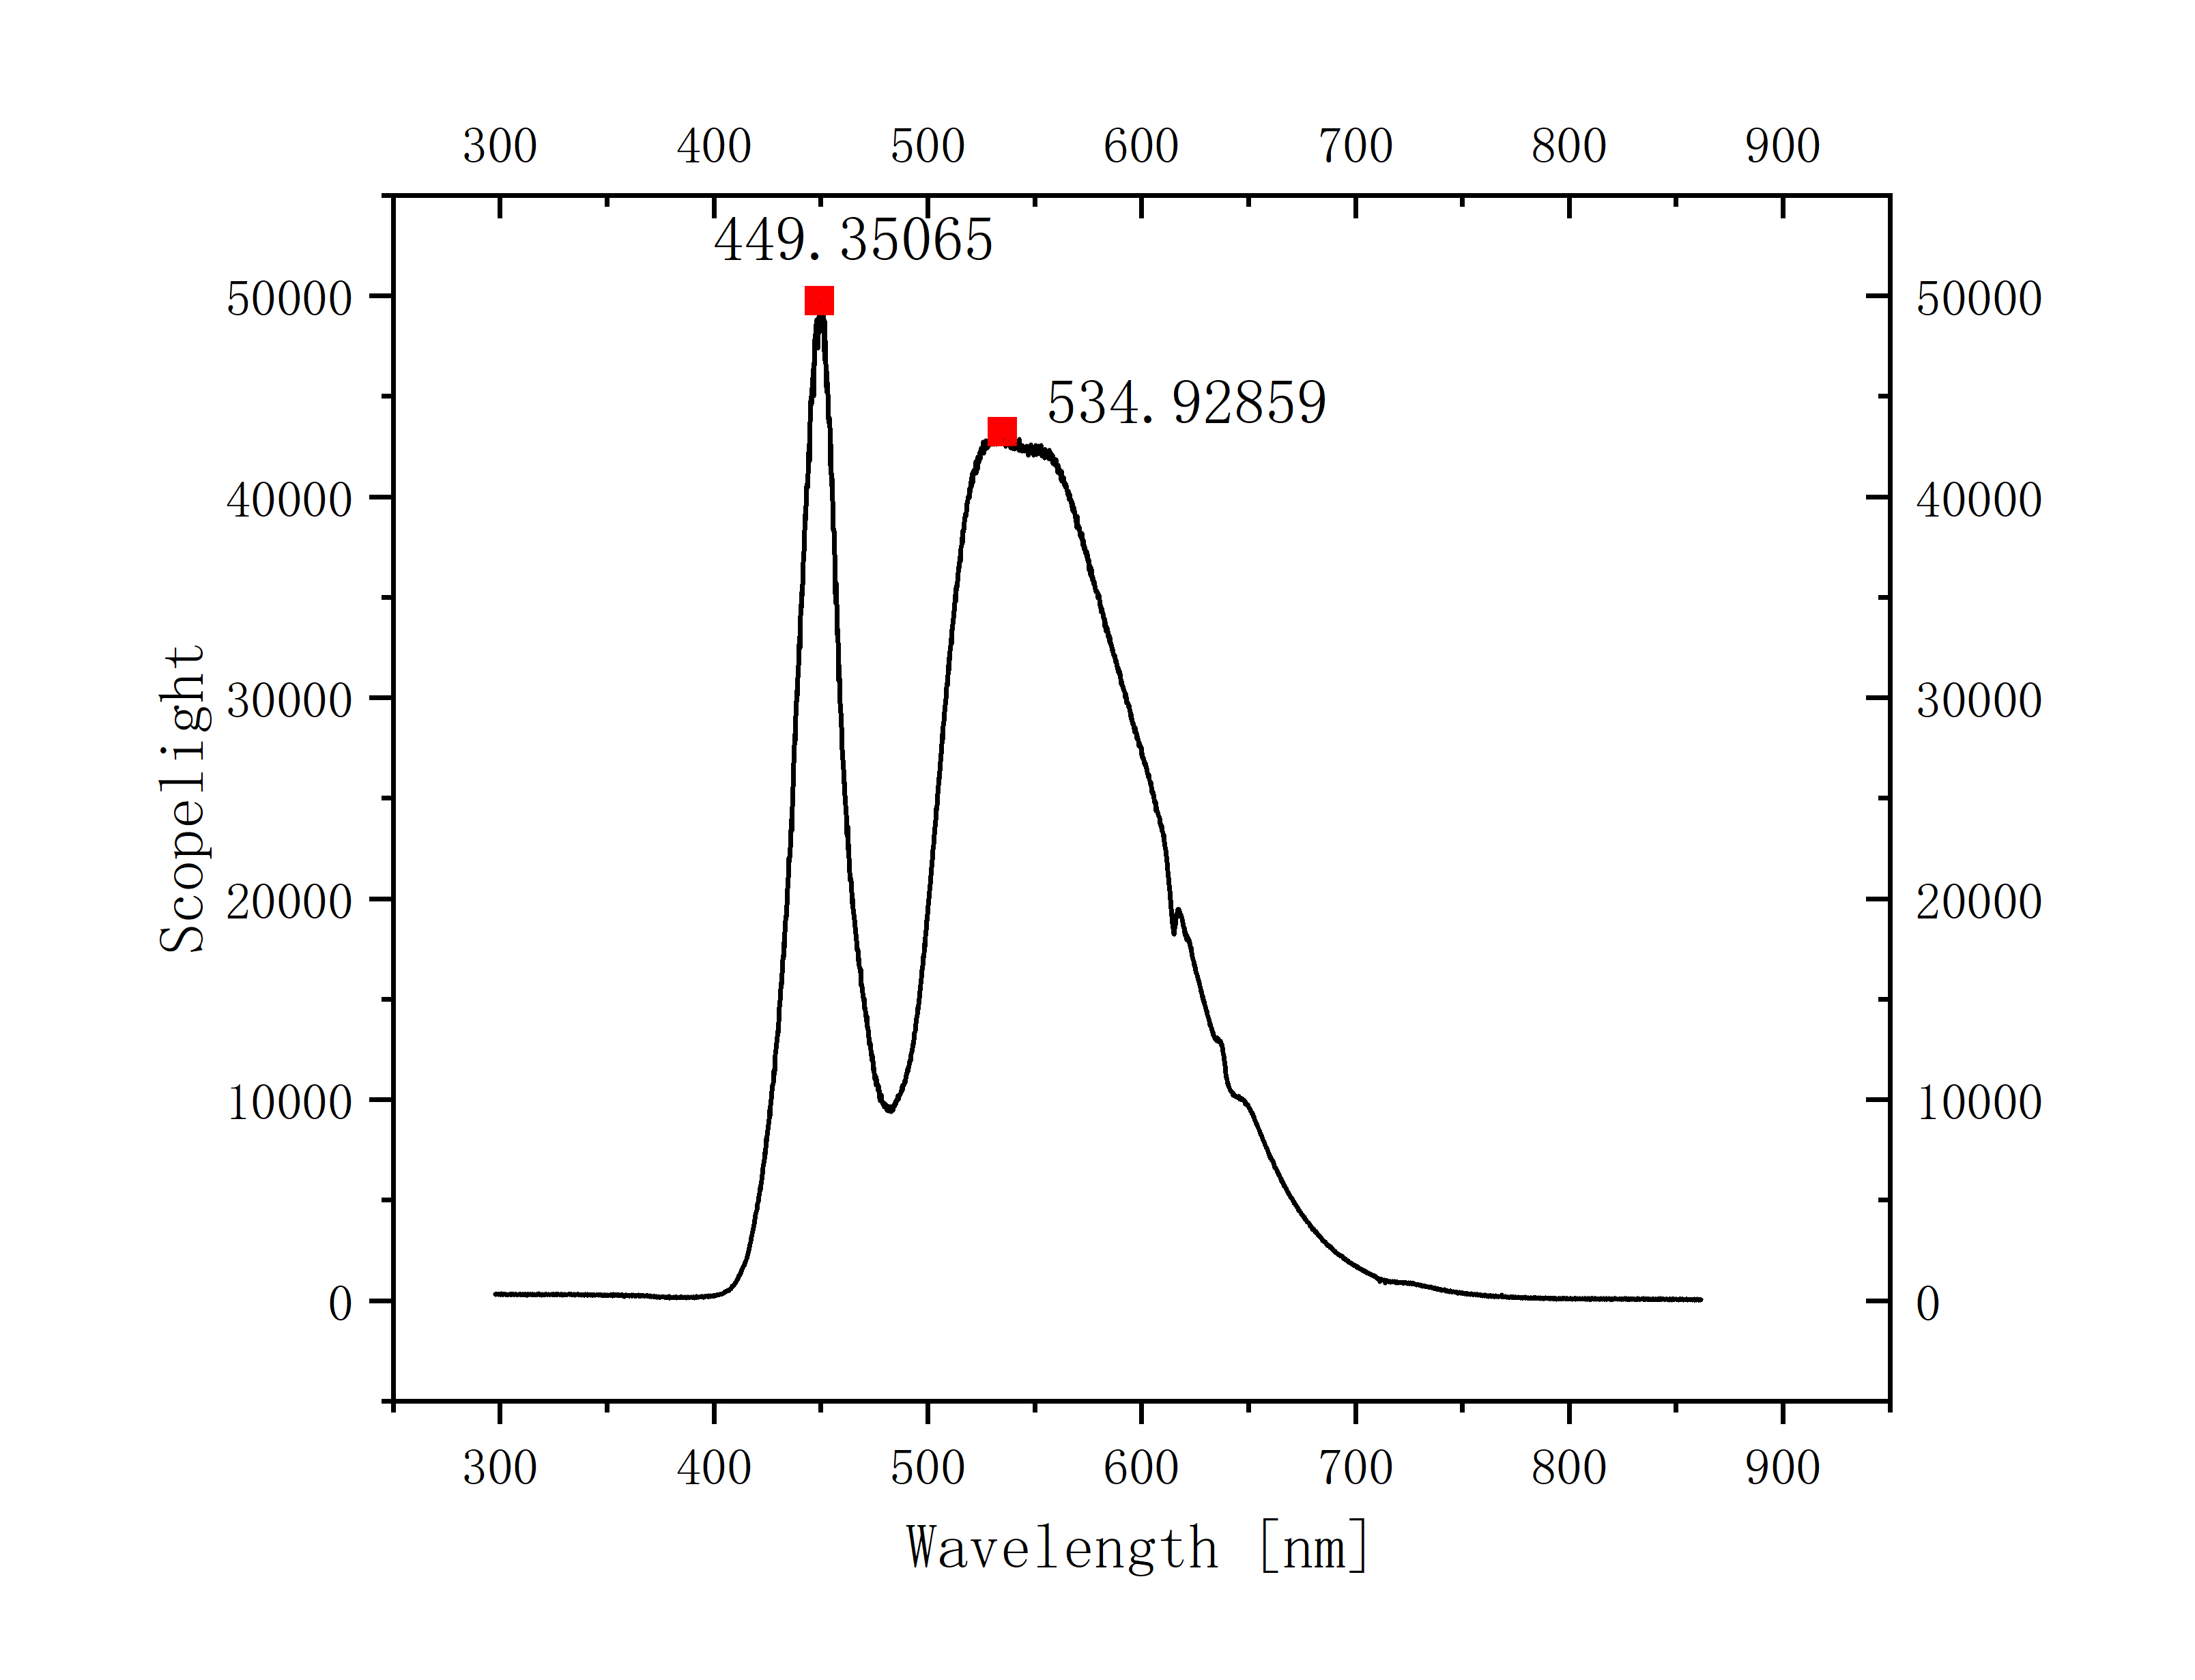
\includegraphics[width=0.7\textwidth]{Lab2_1Gra12.jpg}
			\caption{实验室电灯的发光光谱}
			\label{fig:fig12}
		\end{figure}
		
		这幅处理过的图显示了两个明显的尖峰,分别在大约449.35纳米和534.93纳米。这种离散的发射峰通常是气体放电灯或蒸气灯的特征,比如钠灯或汞灯,因为这些类型的灯具有它们特有的发射线,这些发射线对应于其内部气体原子或离子的特定能级跃迁。
		
		449.35纳米的波长位于蓝色光谱范围内,而534.93纳米则位于绿色光谱范围。一个常见的气体放电光源是汞蒸气灯,它在紫外线范围和可见光范围都有多个发射线,包括蓝色和绿色的光。然而,这两个波长并不精确对应汞蒸气灯最强的线(汞的主要发射线之一是在546.1纳米的绿色光),这意味着可能是其他类型的气体放电或者这两个峰值代表的是通过某种过滤或者涂层处理过的光。
		
		另一种可能是LED灯具,某些LED可以设计成发射特定波长的光。LED技术能够通过使用不同材料和结构来生成特定的光谱特征。例如,某些蓝光LED会利用磷光材料将一部分蓝光转换为黄光,蓝光和黄光混合后产生白光。
		
		由于图中只有两个峰值,而且没有更详细的信息,如光源的材料成分、制造过程或者光谱的完整形态,因此无法给出确切的结论。不过,通常情况下,这样的尖锐峰值往往表明光源是某种形式的气体放电灯,例如荧光灯、氖灯或其他类型的放电管。这些光源使用不同的气体或蒸气来产生特定波长的光。
		
		
		\item 手机闪光灯的光谱分析
		
		同样对测得的数据处理过后,得到如\cref{fig:fig13}所示结果,再结合原图(\cref{fig:figA8})分析,可以发现:
		
		\begin{figure}[htbp]
			\centering
			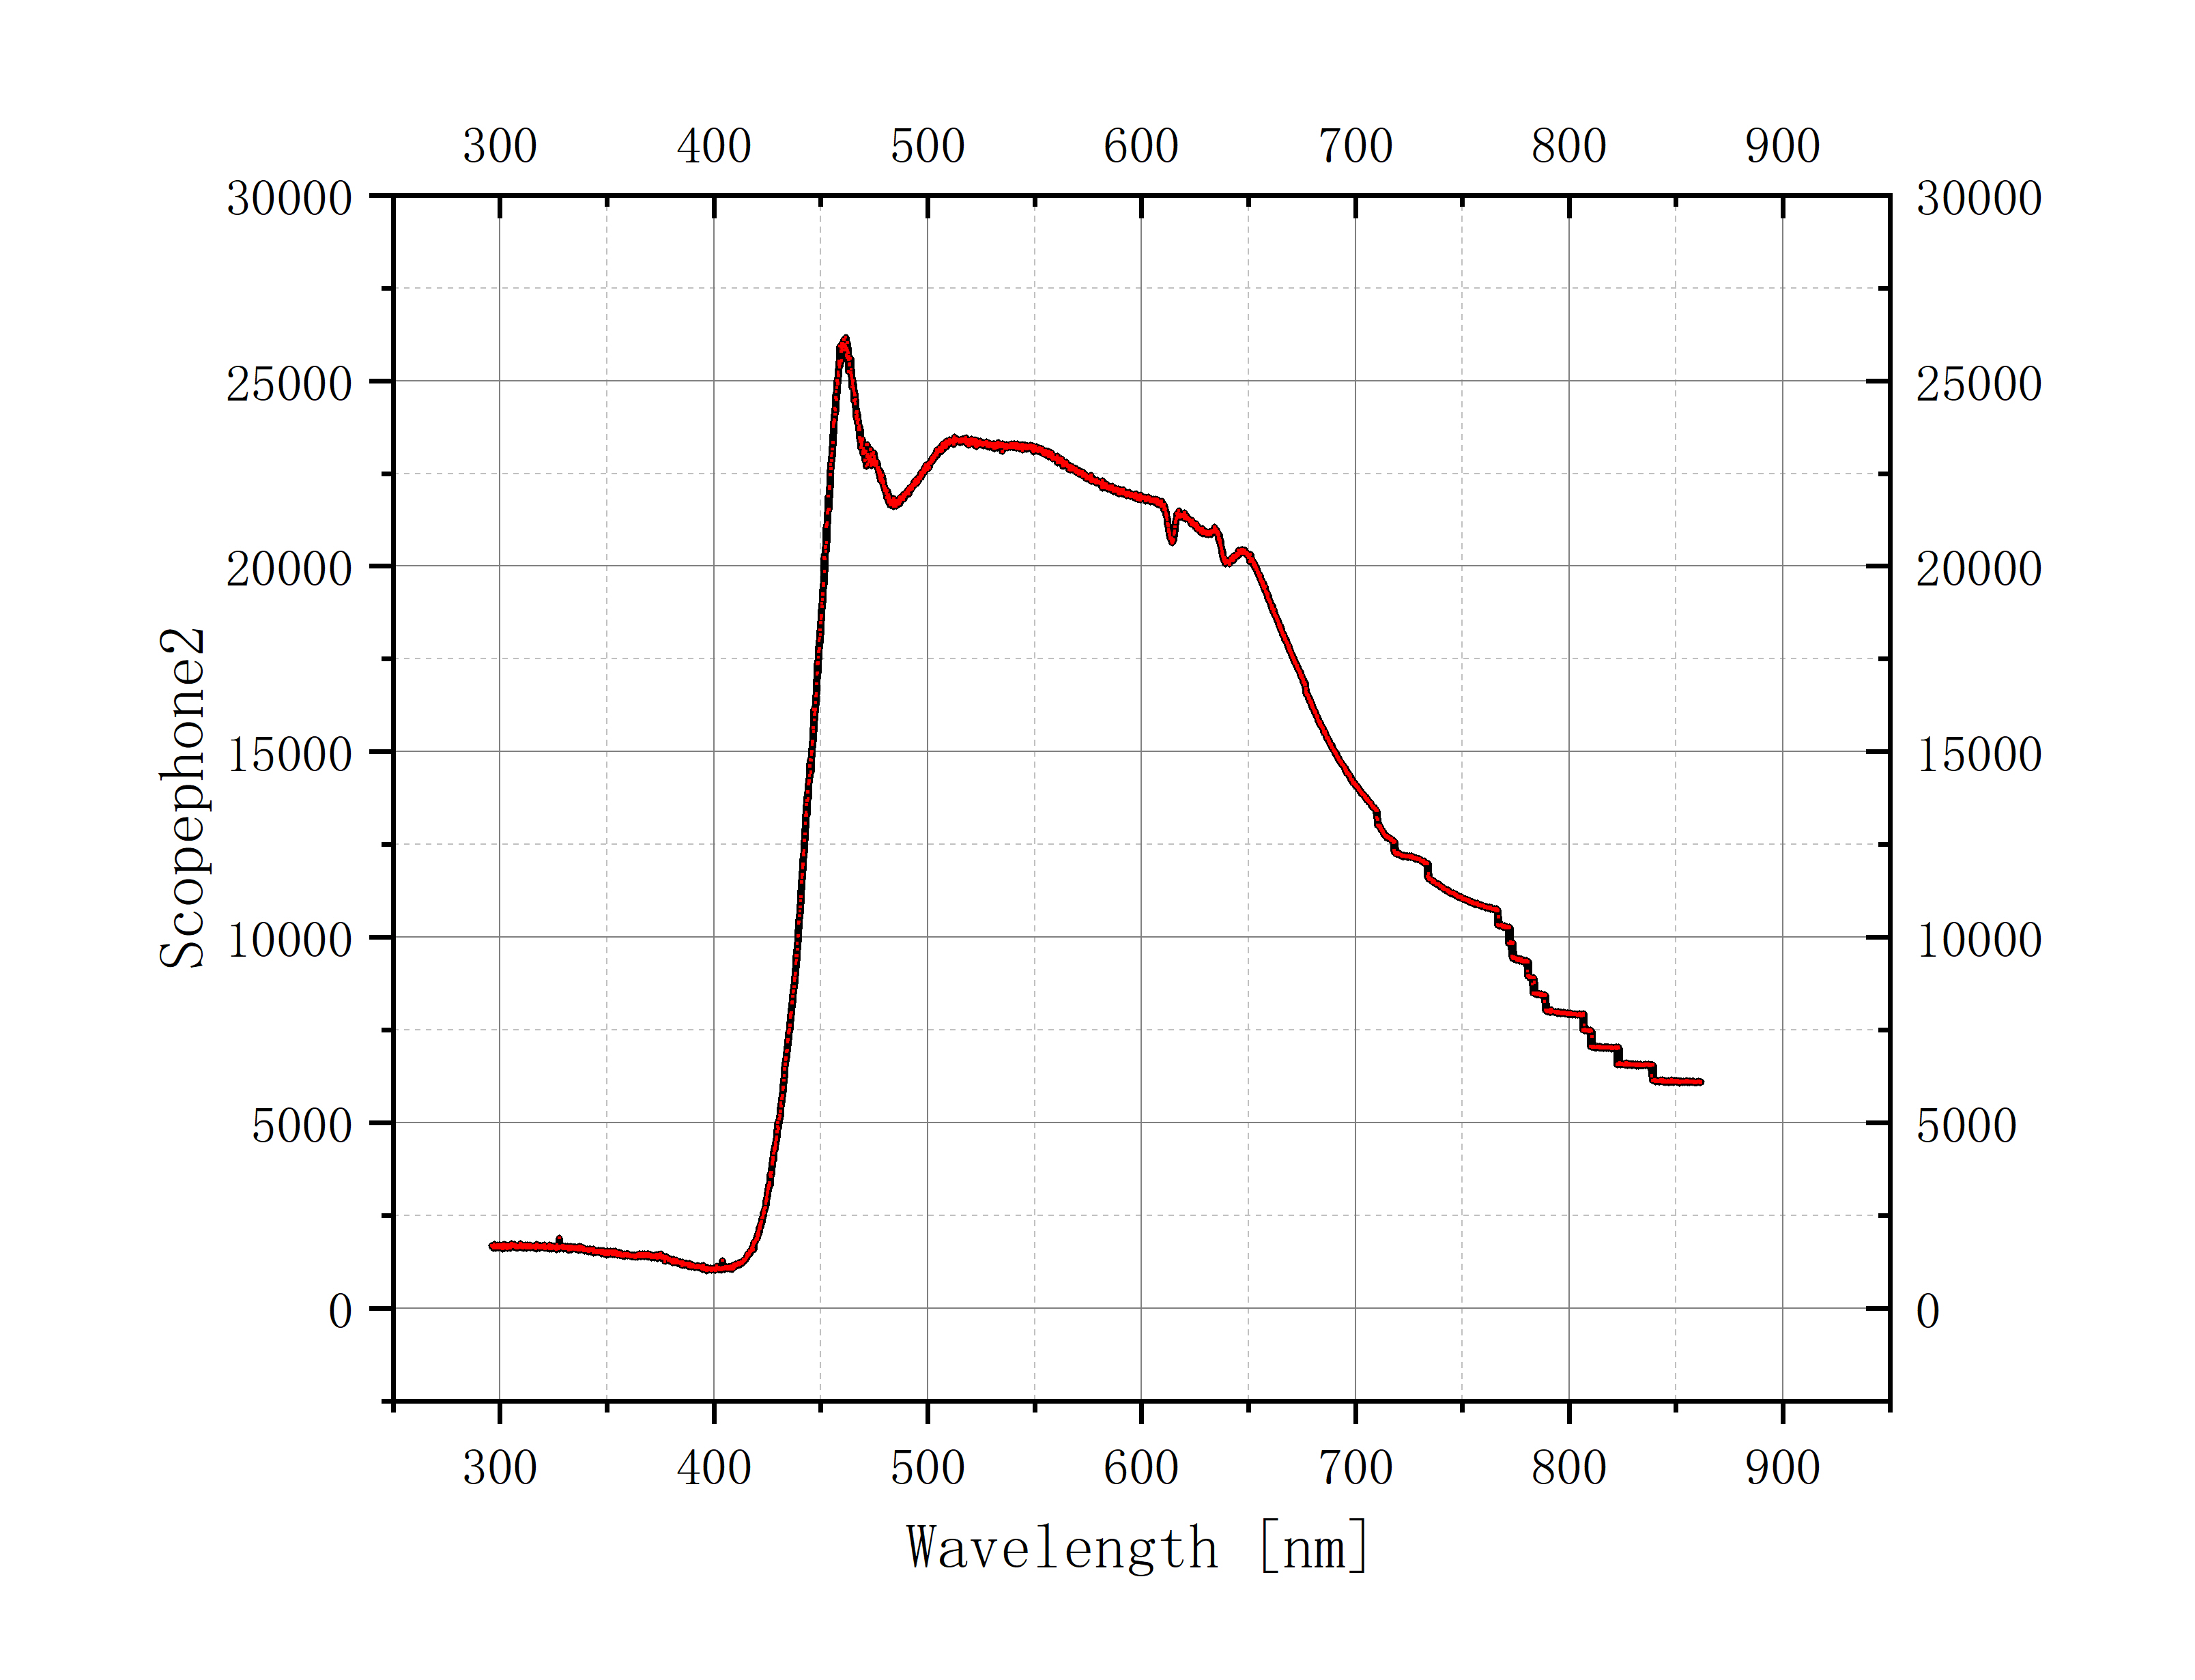
\includegraphics[width=0.7\textwidth]{Lab2_1Gra13.jpg}
			\caption{手机闪光灯的发光光谱}
			\label{fig:fig13}
		\end{figure}
		
		在紫外区域(UVA),图中以斜纹背景表示该区域不在可见光范围内,从紫外区开始光强逐渐增加,达到可见光蓝色波段的一个尖峰,之后光强度下降,然后在绿色到黄绿色波段出现一个小的峰值,随后继续下降。
		
		这个光谱呈现了连续的分布,没有特别尖锐的发射线,这通常表明光源是由LED(发光二极管)产生的,因为LED发光通常会产生宽带的光谱,而不是像气体放电灯那样有特定的谱线。手机闪光灯通常采用白色LED,它们结合了蓝色LED芯片和黄色荧光粉来生成白光。
		
		蓝色波段的峰值代表了LED芯片的原生发光,而随后的光谱宽带可能是由黄色荧光粉的发光与蓝色光混合产生的。整个光谱覆盖了从蓝光到红光的大部分可见光范围,这样的混合使得光源产生了近似白色的光。
		
		总的来说,这张光谱图显示了一个相对平滑的曲线,而不是尖锐的线或峰,这支持了这是一种LED光源的观点,其特点是宽广的发光波长范围。光谱中没有显著的紫外线或红外线部分,这符合大多数手机闪光灯设计的目标,即提供适合照相的光范围。
				
		\item 手机屏幕的光谱分析
		
		对于手机屏幕的发光光谱,我们做相同的处理,得到:
		
		\begin{itemize}
			\item 在蓝光区域(大约465.40纳米)有一个尖锐的峰,这对于基于蓝色LED的白光发射具有典型意义,蓝色LED通常是通过蓝色发光二极管与黄色荧光粉结合产生白光的。
			\item 在绿光区域(约530.21纳米)也有一个尖峰,这通常是由荧光粉发出,其将部分蓝光转换成绿光。
			\item 红光区域(约620.70纳米)的尖峰可能是由另一种荧光粉发出,将部分蓝光转换成红光,或者是由红色LED直接产生。
		\end{itemize}
		
		\begin{figure}[htbp]
			\centering
			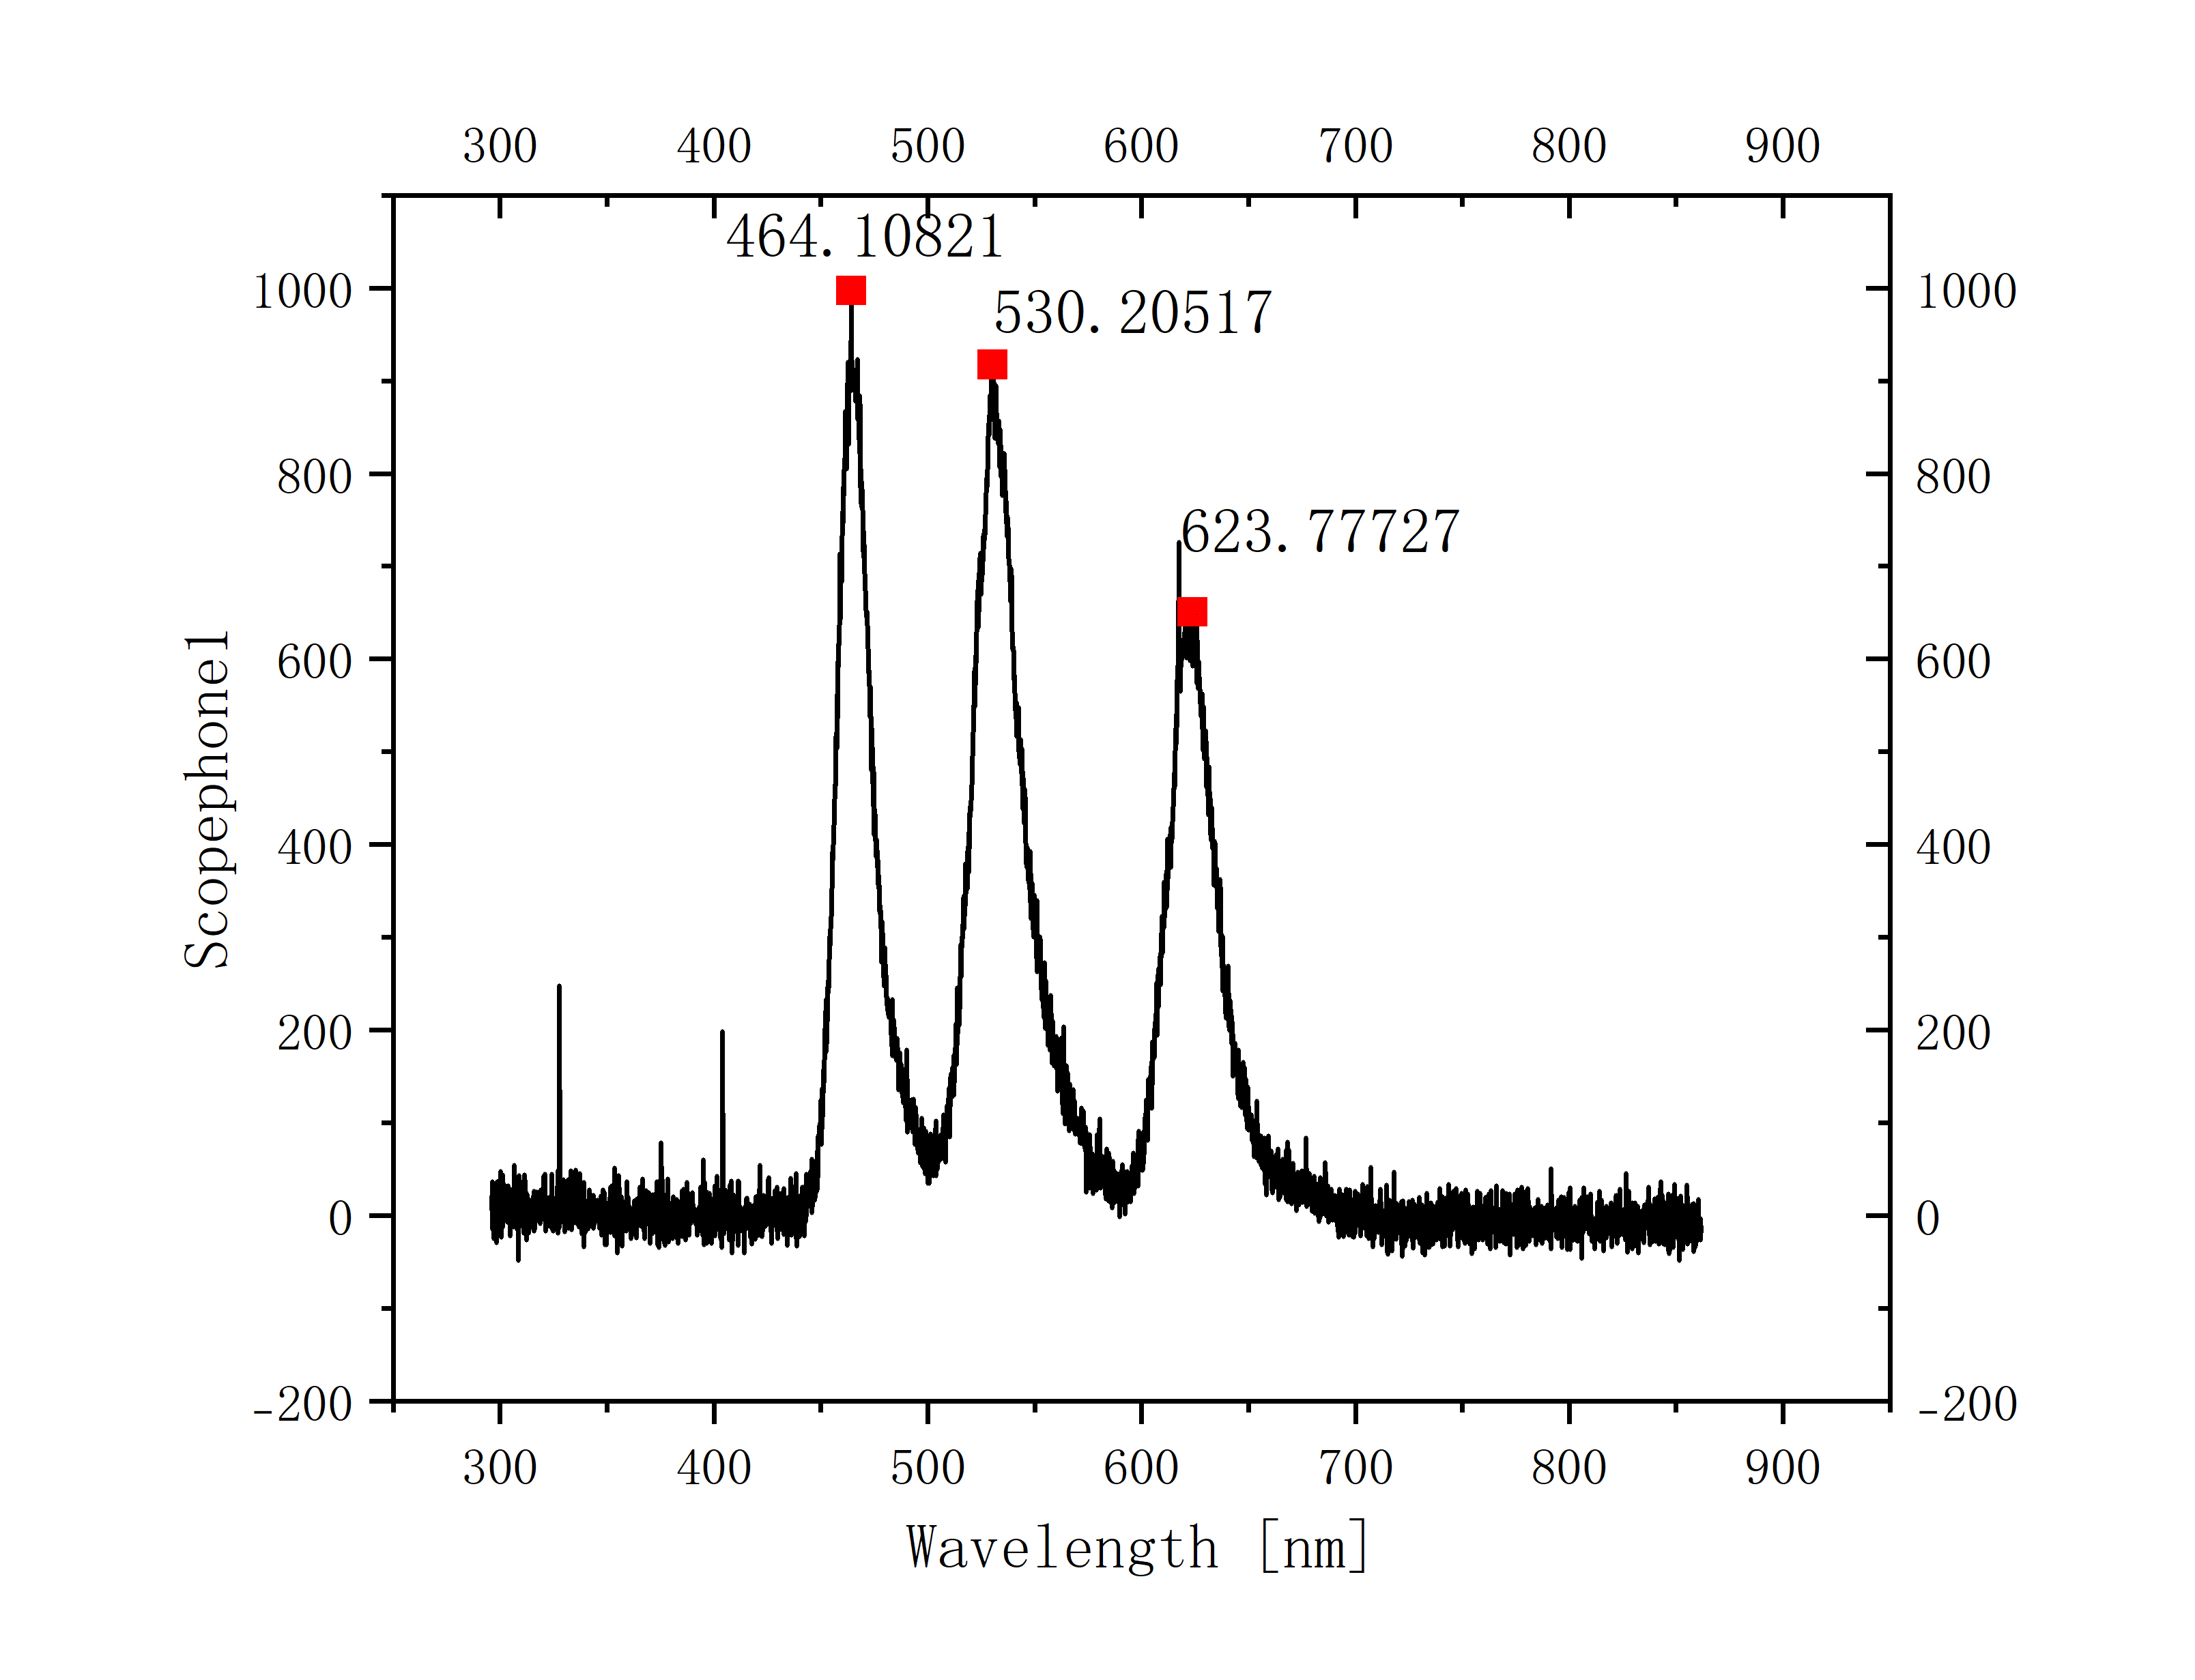
\includegraphics[width=0.7\textwidth]{Lab2_1Gra14.jpg}
			\caption{手机屏幕的发光光谱}
			\label{fig:fig14}
		\end{figure}
		
		从这张处理过的光谱图(\cref{fig:fig14})中,我们可以观察到三个明显的发射峰,分别在大约464.10纳米(蓝色光区域)、530.21纳米(绿色光区域)和623.78纳米(红色光区域)。这些峰值反映了手机屏幕在这些特定波长的光发射的强度。
		
		智能手机屏幕,包括iPhone 13 mini,通常使用LED或OLED技术来生成不同颜色的光。对于LED屏幕,这通常涉及到蓝色LED发光体和不同荧光材料的组合,以产生红色和绿色的光,从而混合形成白色背光。对于OLED屏幕,不同颜色的有机材料会直接发光。
		
		这些峰值应该反映了iPhone 13 mini屏幕用于形成图像的基本颜色组件的发光特性。对于iPhone 13 mini,苹果官方给出的标准参数中提到,其屏幕使用了OLED技术,这意味着每个像素是由发光的有机材料组成,能够单独开启和关闭,以产生所需的颜色。
		
		光谱图中的数据与iPhone 13 mini使用的OLED技术相匹配,因为OLED屏幕可以产生清晰的发射峰,表示纯净色彩的发光。		
		
	\end{enumerate}
	
	%
	\clearpage
	\subsubsection{Beer定律验证}
	利用测量得到的数据,出于噪声太大的原因,我分别通过编写Python脚本和手动的方式,选出了各浓度三个峰值,如\cref{fig:fig15}和\cref{fig:fig16}所示。
	
	\begin{figure}[htbp]
		\centering
		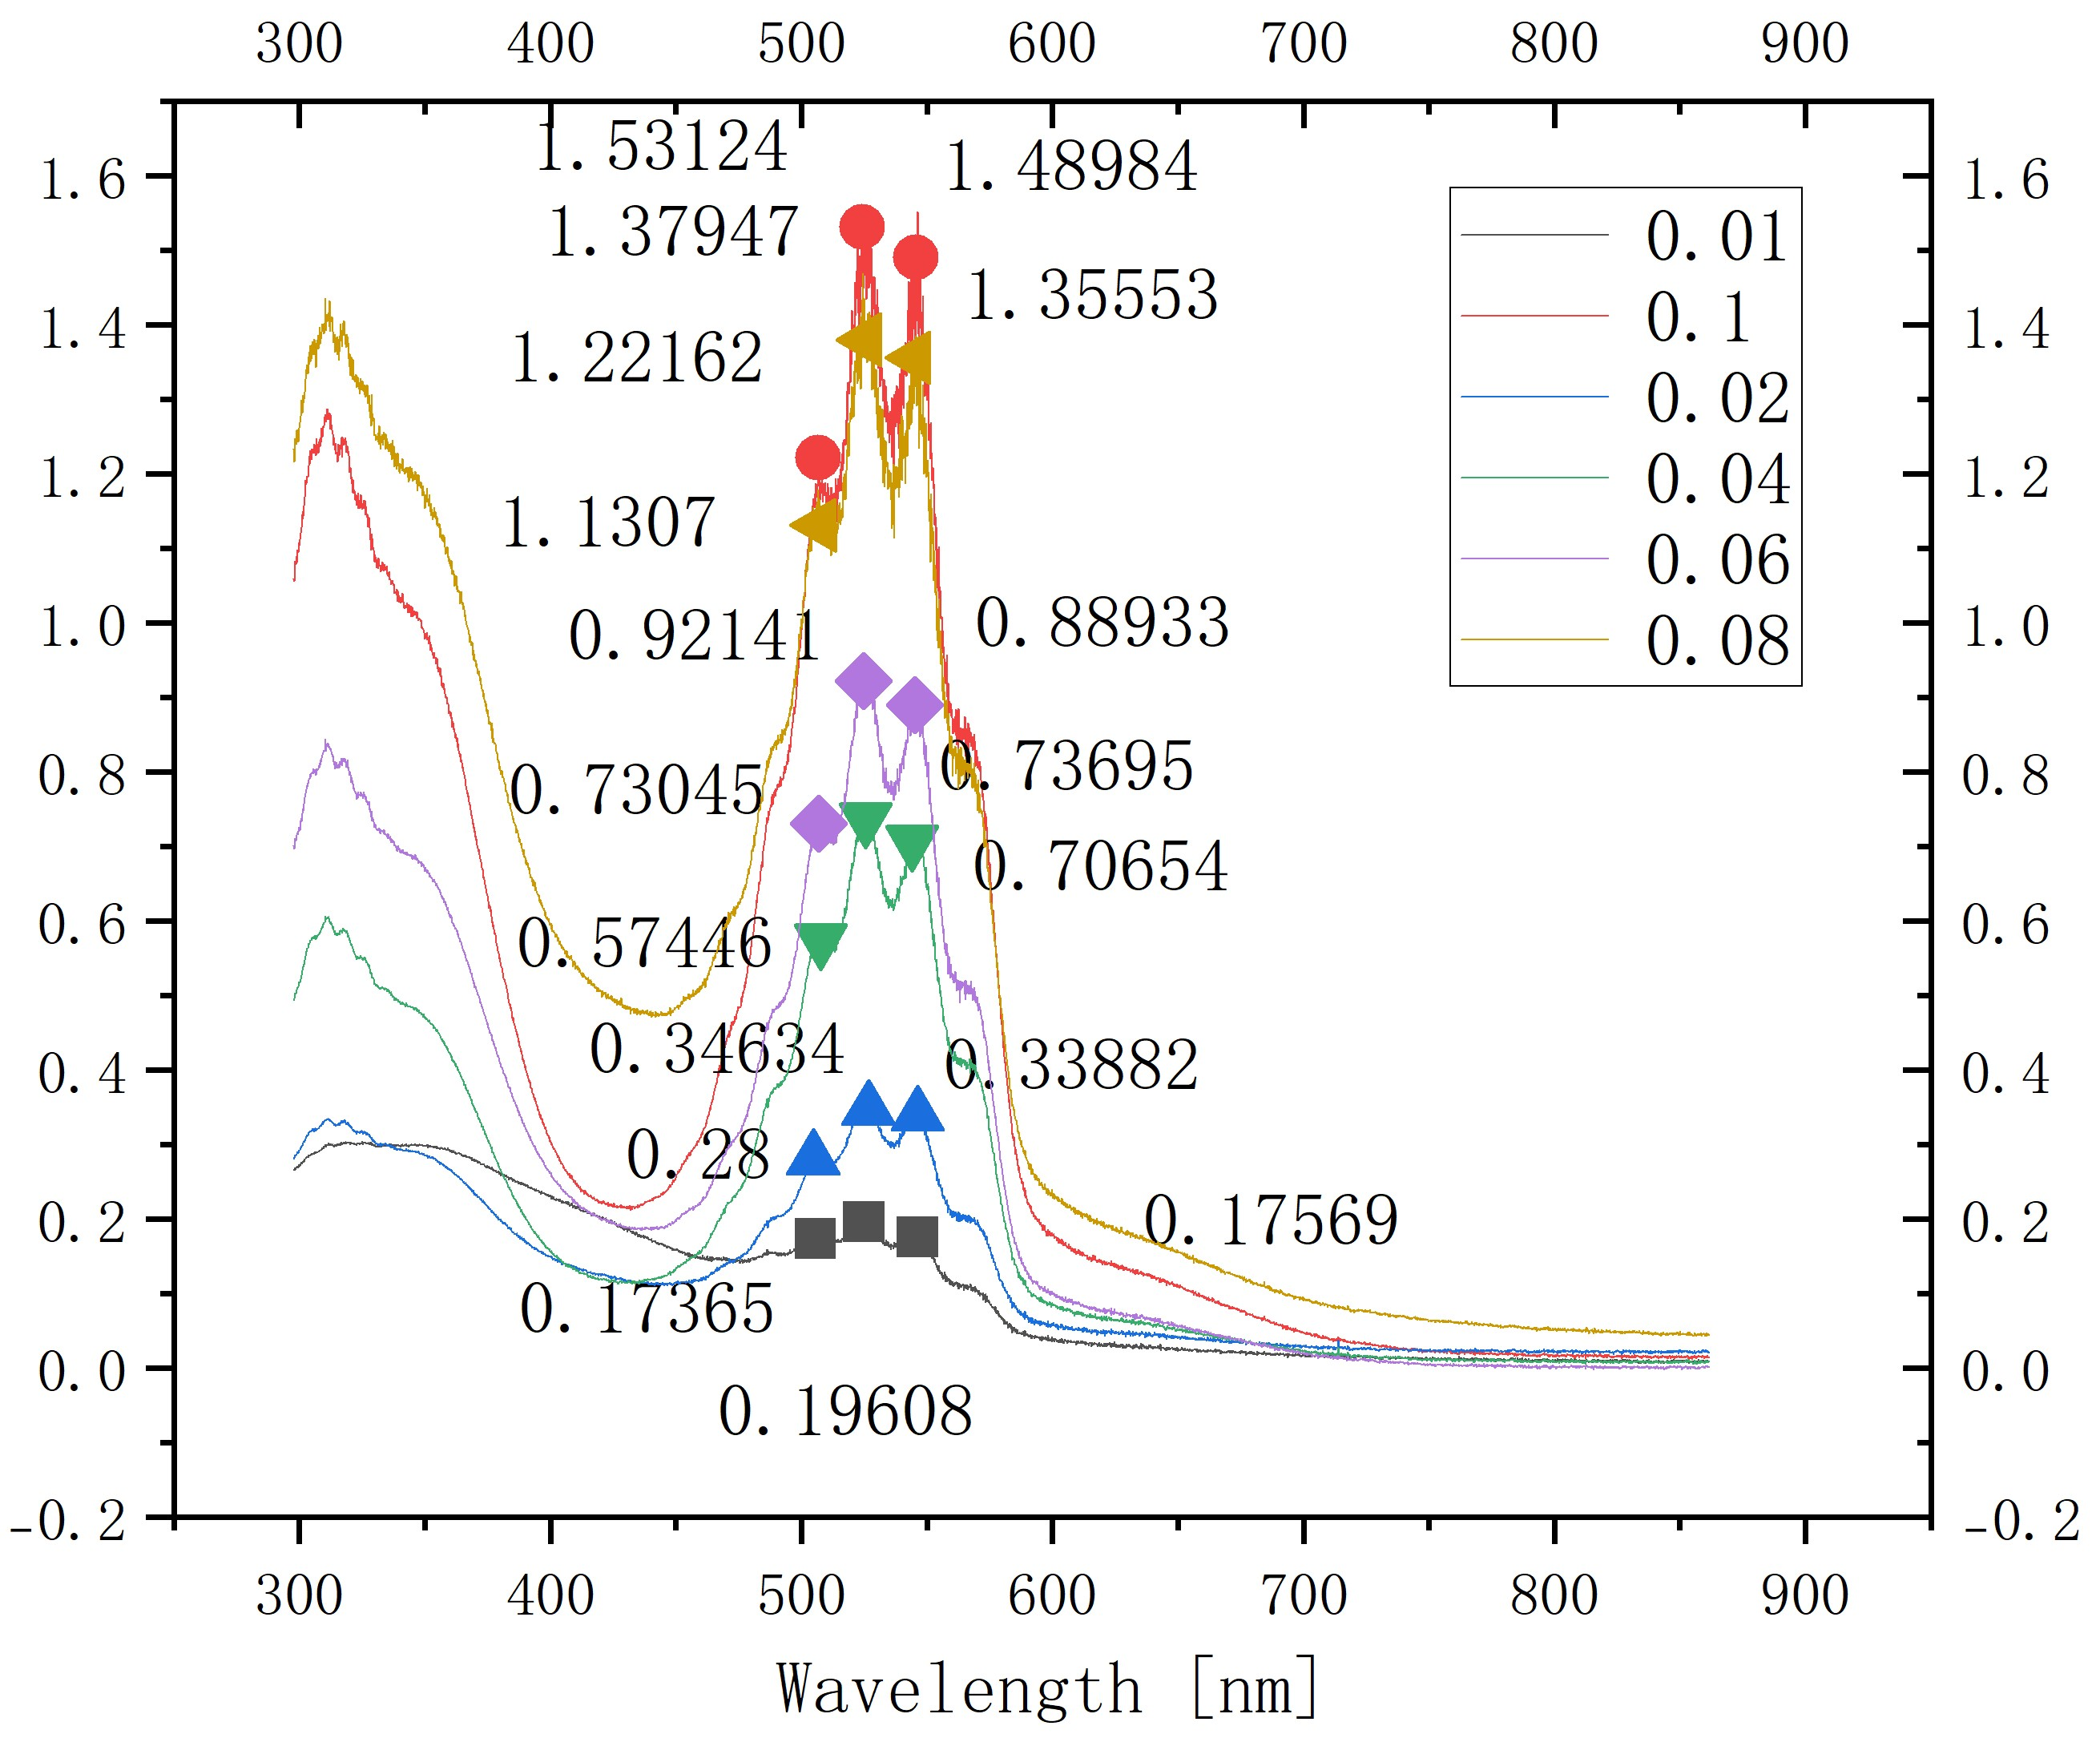
\includegraphics[width=0.48\textwidth]{Lab2_1Gra15.jpg}
		\caption{用Origin进行手动寻峰结果}
		\label{fig:fig15}
	\end{figure}
	
	\begin{figure}[htbp]
		\centering
		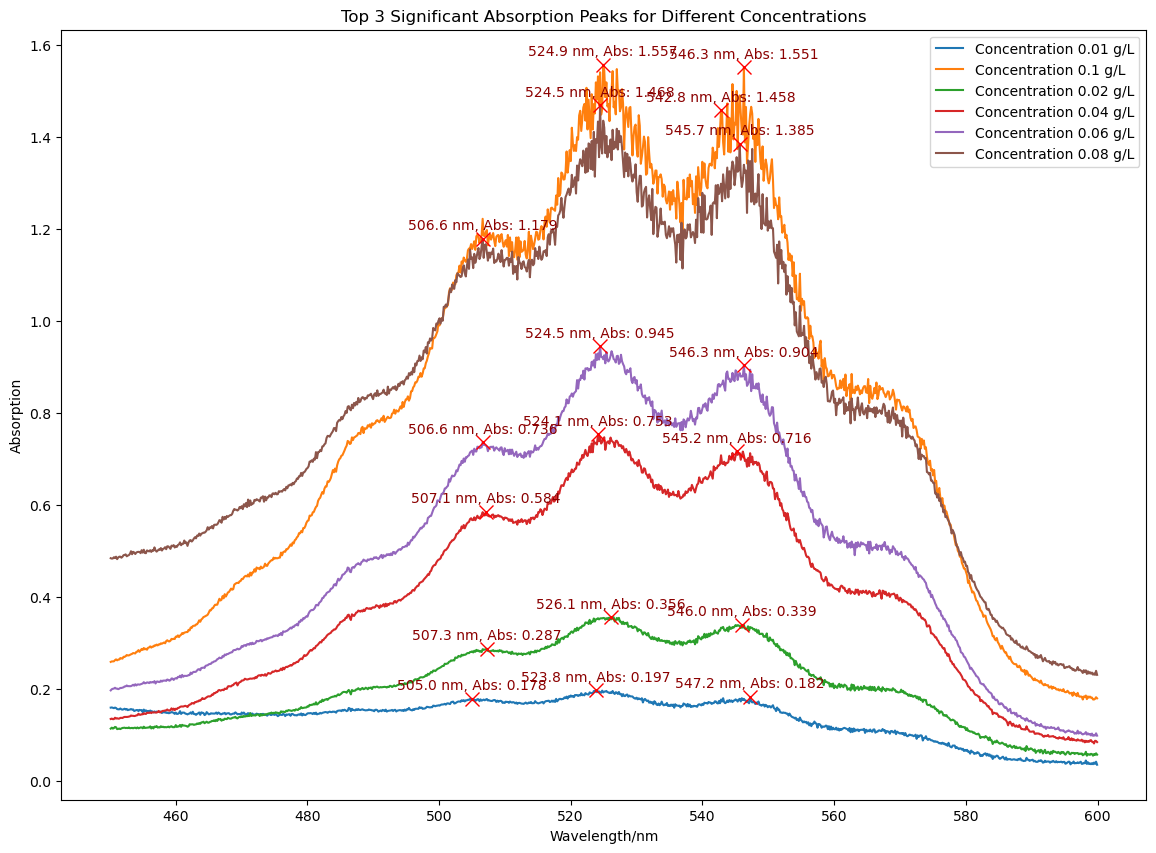
\includegraphics[width=0.65\textwidth]{Lab2_1Gra16.png}
		\caption{脚本寻峰结果}
		\label{fig:fig16}
	\end{figure}
	
	\clearpage
	接下来我选取了其中一些数据来验证Beer定律,结果如下(\cref{tab:tab2})。
	
	\begin{table}[htbp]
		\centering
		\caption{吸收率随浓度变化的数据}
		\begin{tabular}{|c|c|c|c|}
			\hline
			浓度(g/L) & 吸收率1 & 吸收率2 & 吸收率3 \\
			0.01  & 0.174 & 0.197 & 0.182 \\
			0.02  & 0.280 & 0.356 & 0.339 \\
			0.04  & 0.574 & 0.753 & 0.716 \\
			0.06  & 0.730 & 0.945 & 0.904 \\
			0.08  & 1.131 & 1.468 & 1.385 \\
			0.10  & 1.222 & 1.557 & 1.551 \\
			\hline
		\end{tabular}%
		\label{tab:tab2}%
	\end{table}%
	
	如\cref{fig:fig17}所示,对应于从左起选取的第一个峰,从图中可以看出,斜率为12.227,相关系数达到0.991,说明数据点有着较好的线性关系。
	
	\begin{figure}[htbp]
		\centering
		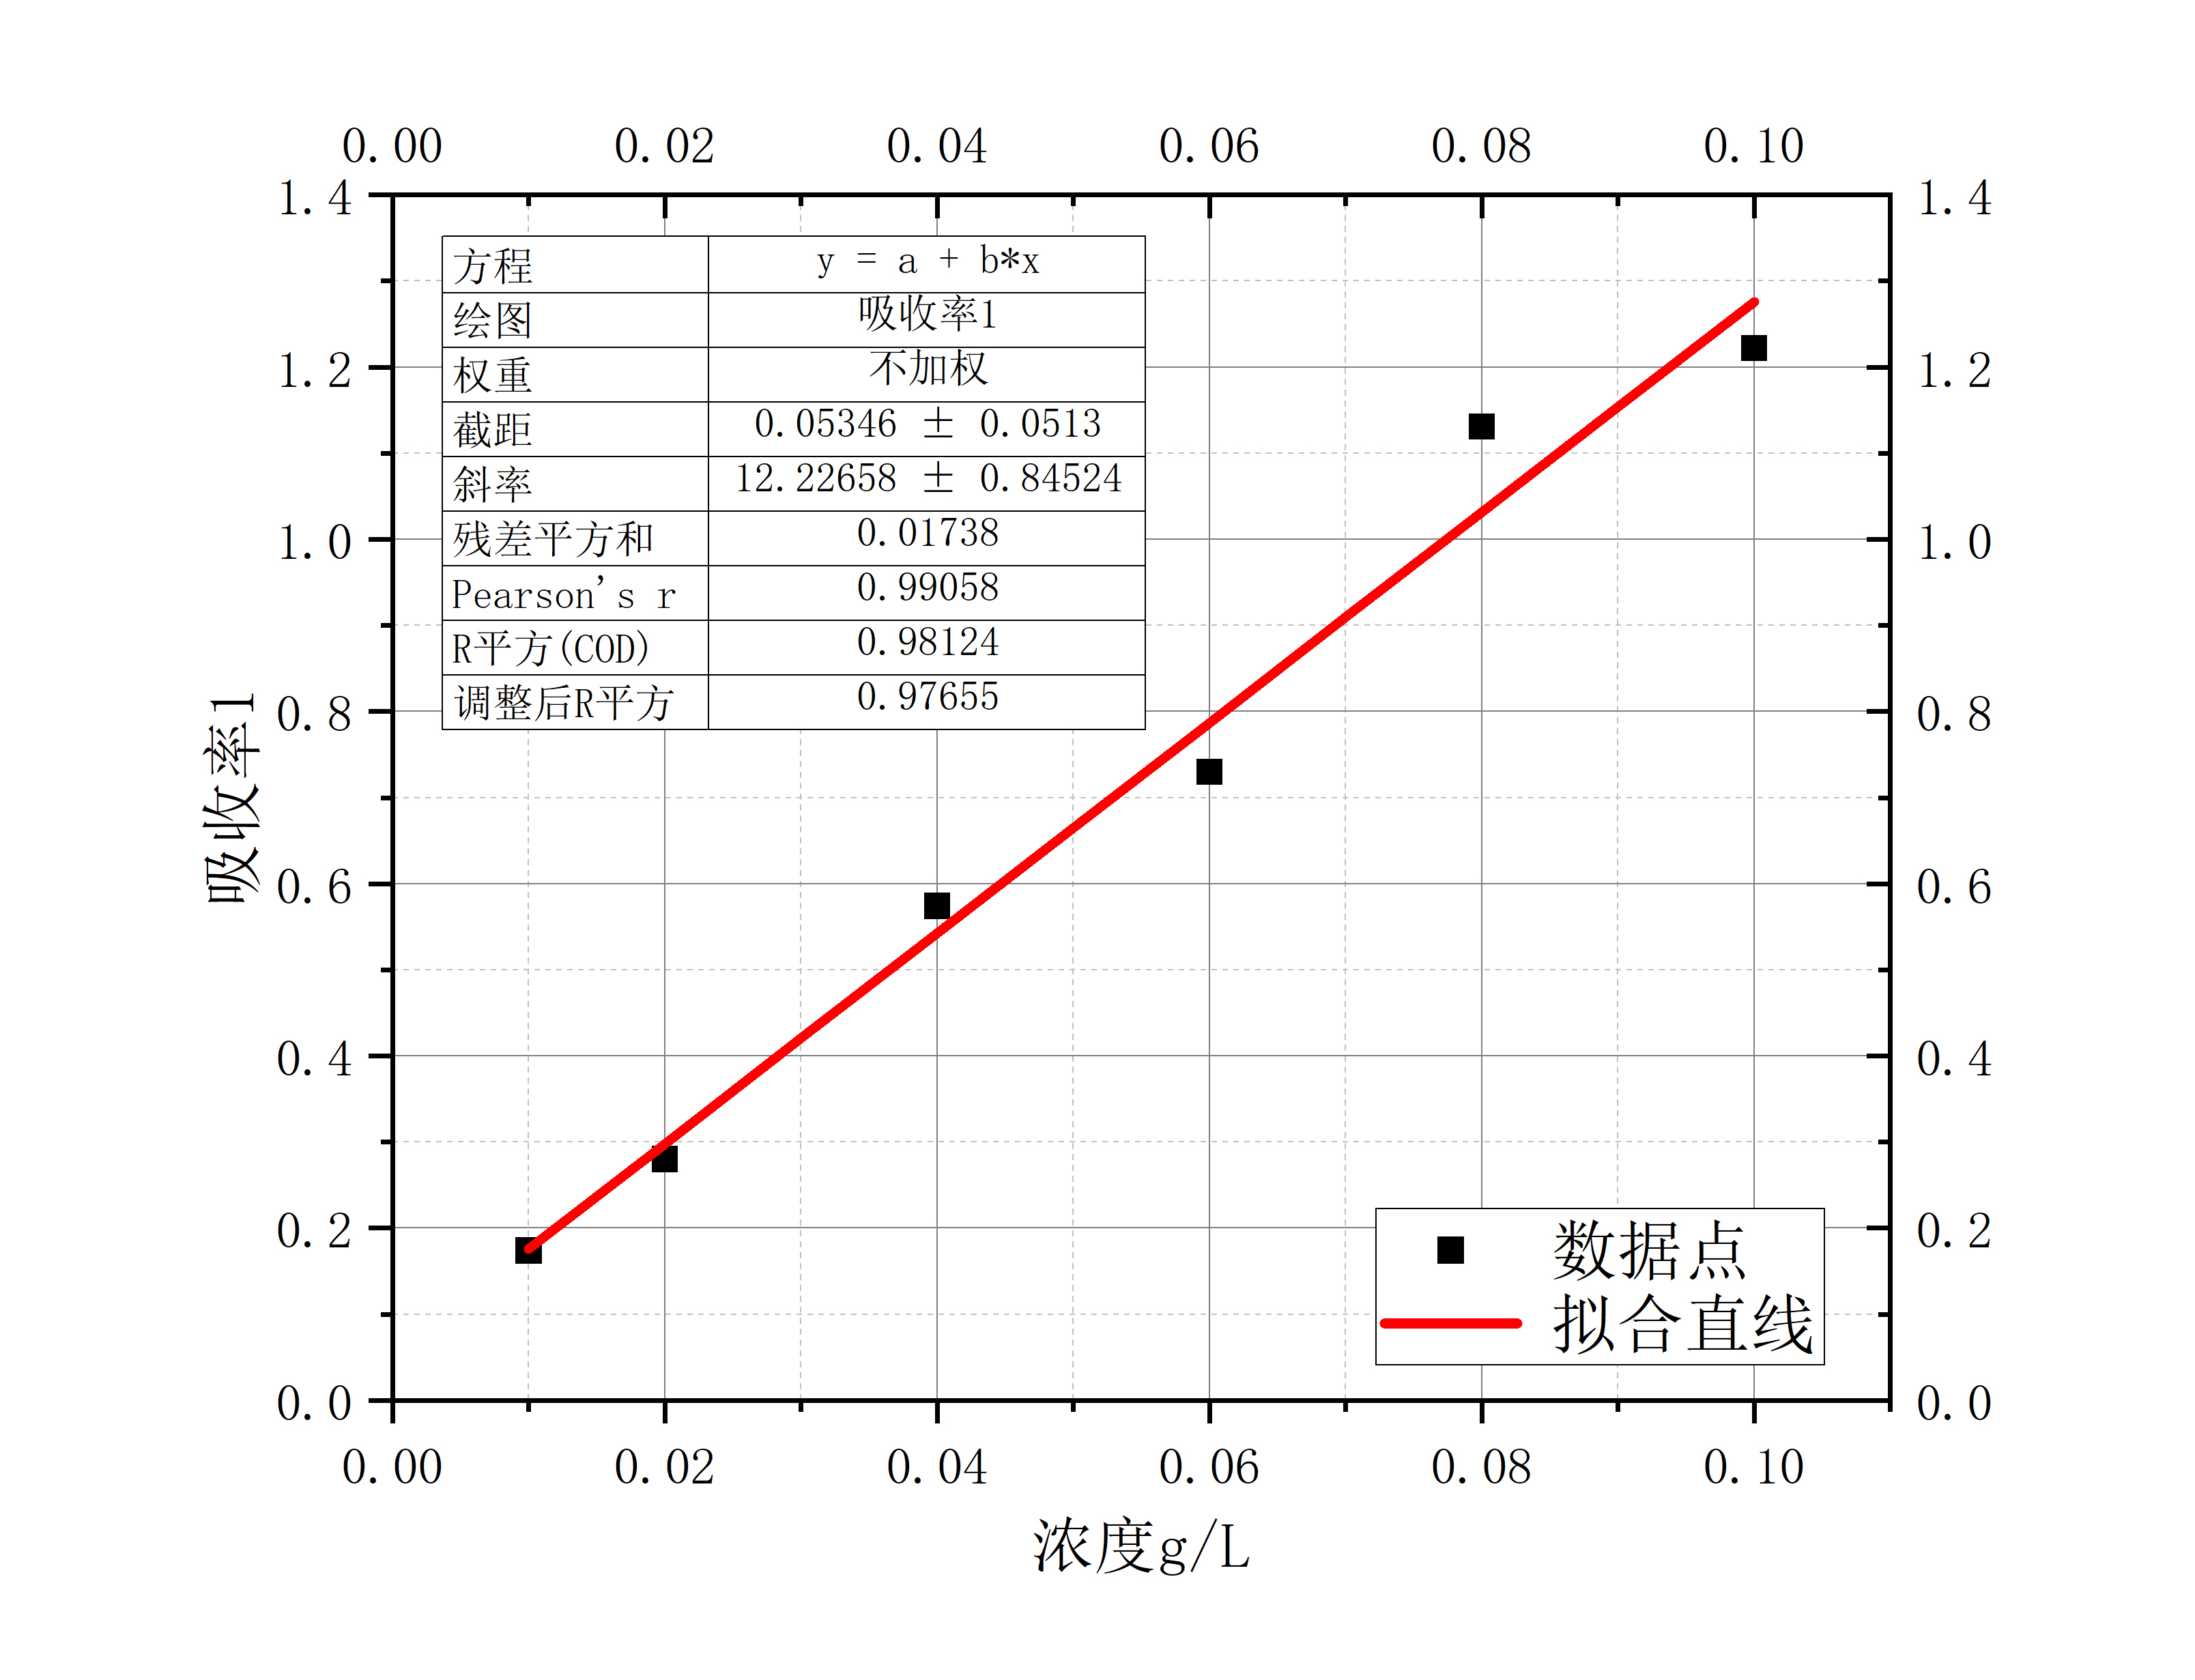
\includegraphics[width=0.7\textwidth]{Lab2_1Gra17.jpg}
		\caption{Beer定律验证1}
		\label{fig:fig17}
	\end{figure}
	
	\clearpage
	如\cref{fig:fig18}所示,对应于从左起选取的第二个峰,从图中可以看出,斜率为15.856,相关系数达到0.988,说明数据点有着较好的线性关系。
	
	\begin{figure}[htbp]
		\centering
		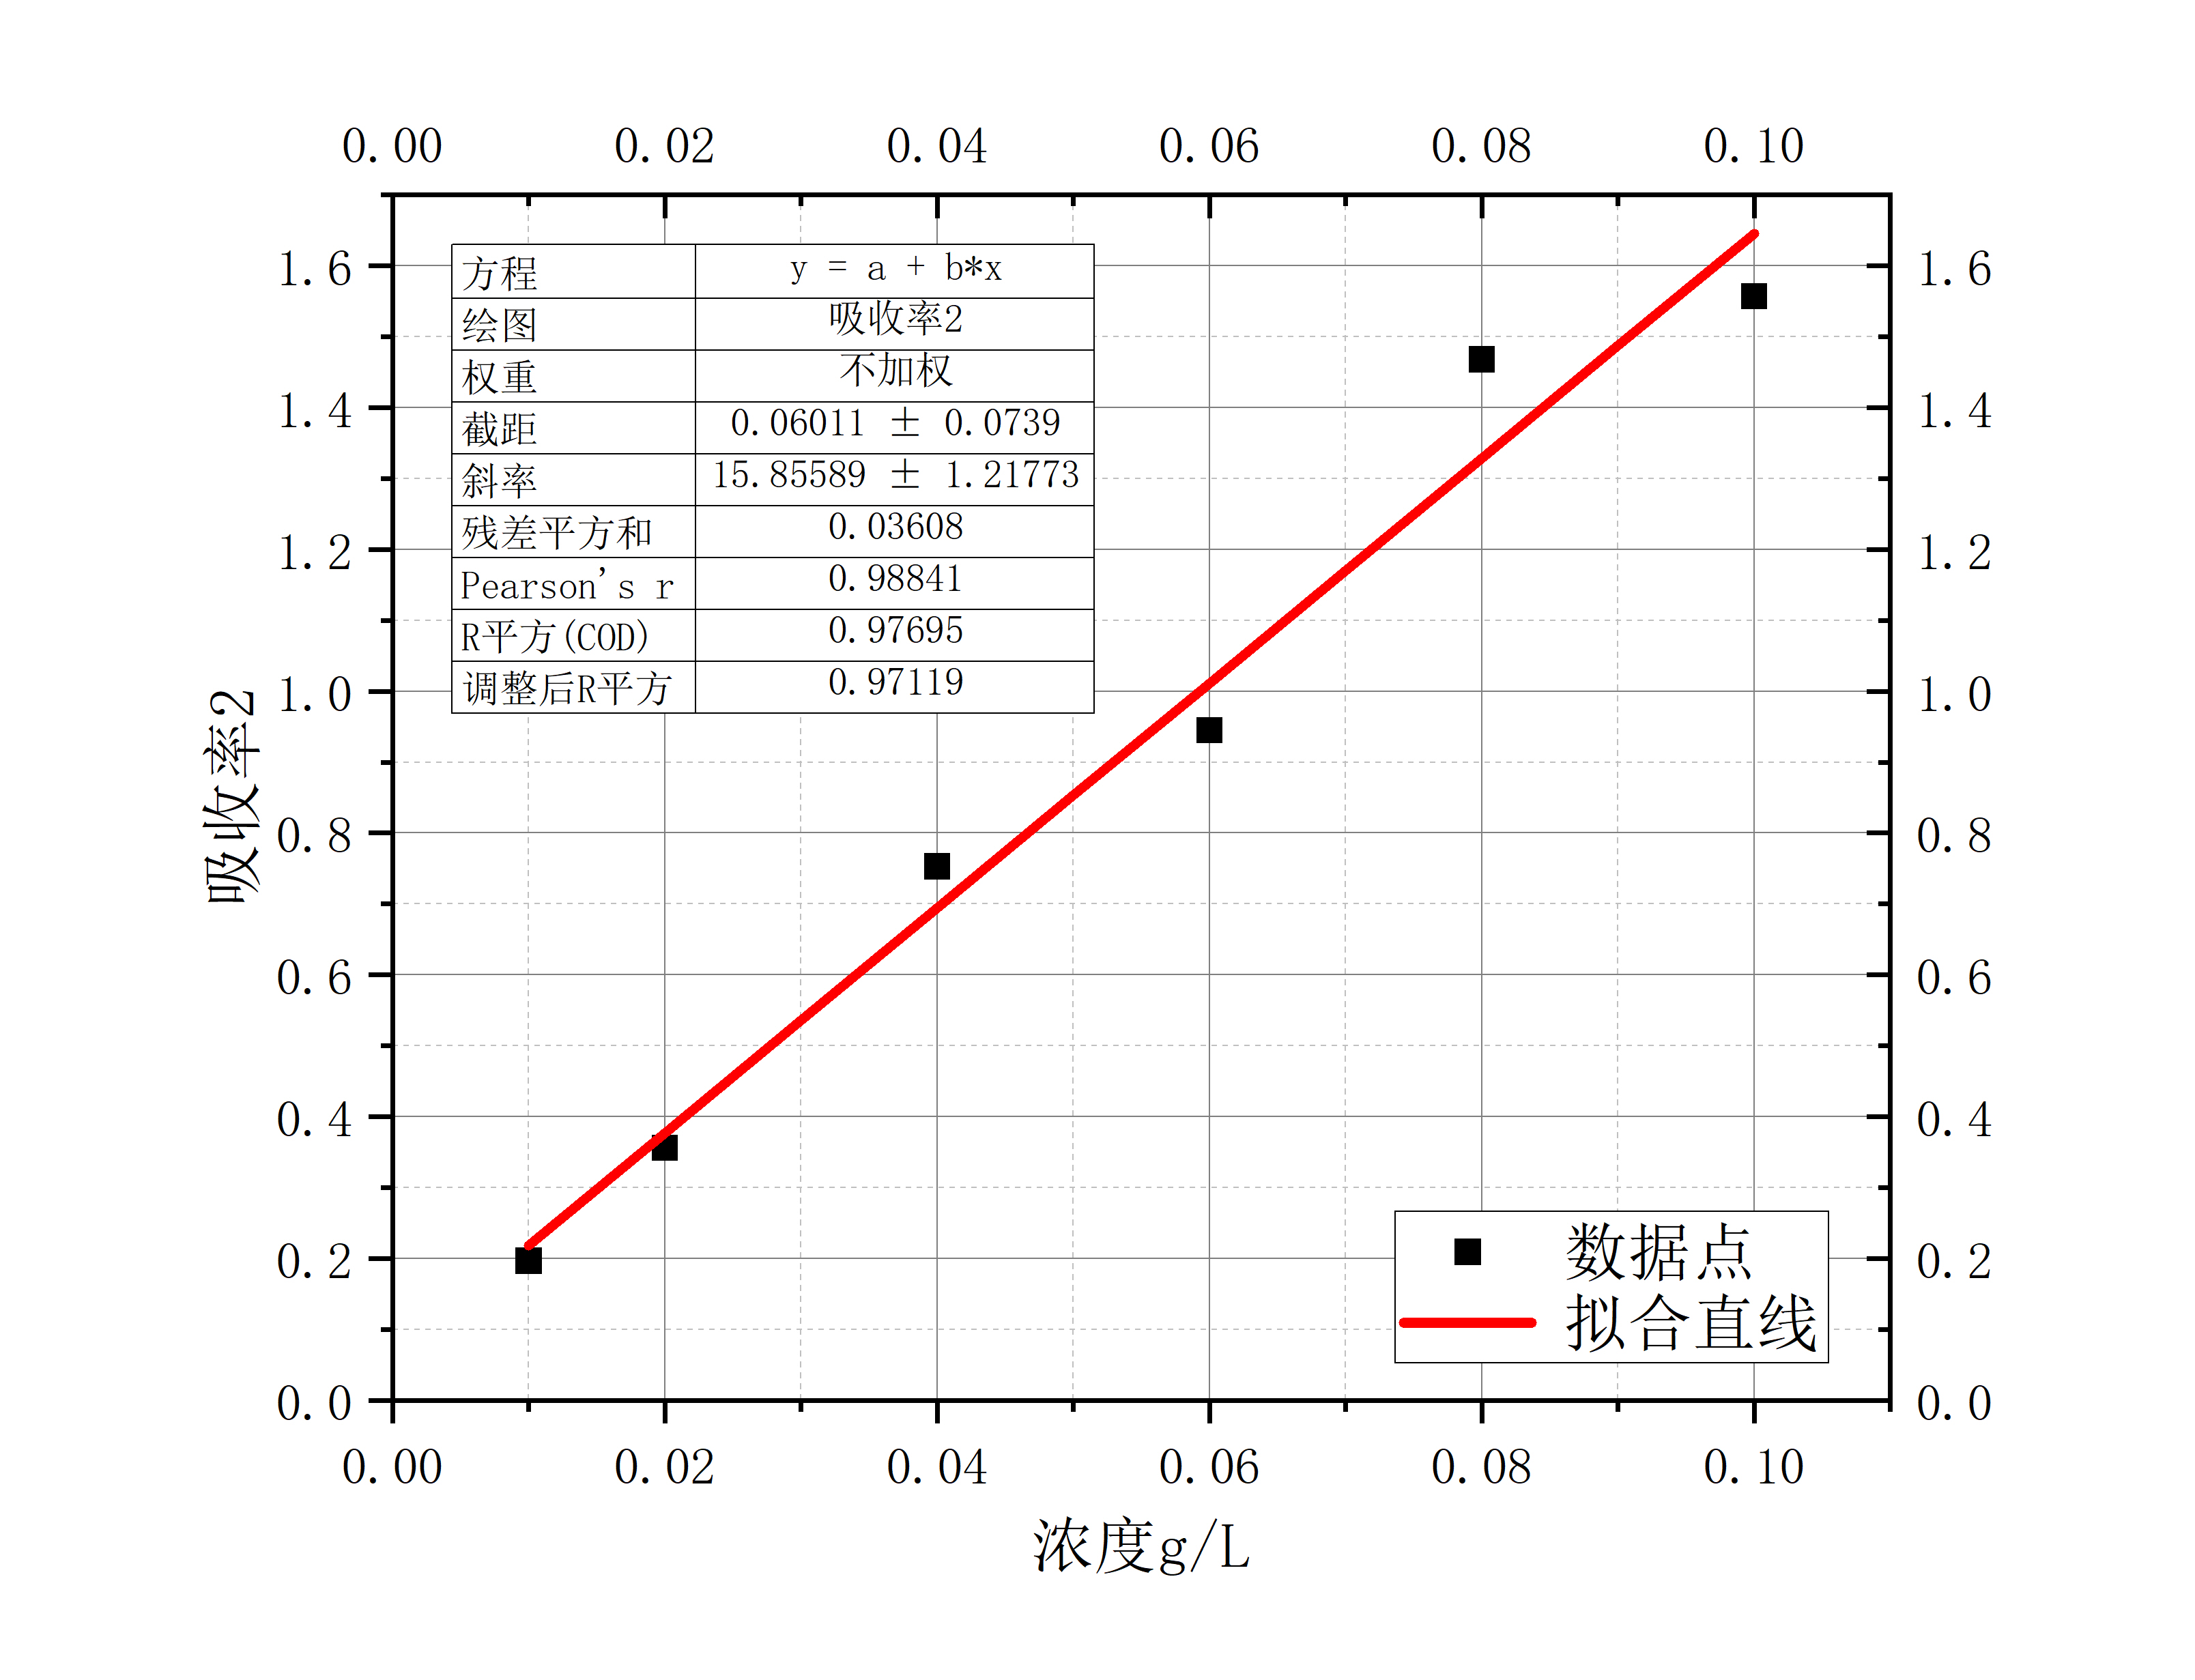
\includegraphics[width=0.55\textwidth]{Lab2_1Gra18.jpg}
		\caption{Beer定律验证2}
		\label{fig:fig18}
	\end{figure}
	
	如\cref{fig:fig19}所示,对应于从左起选取的第三个峰,从图中可以看出,斜率为15.627,相关系数达到0.993,说明数据点有着较好的线性关系。
	
	\begin{figure}[htbp]
		\centering
		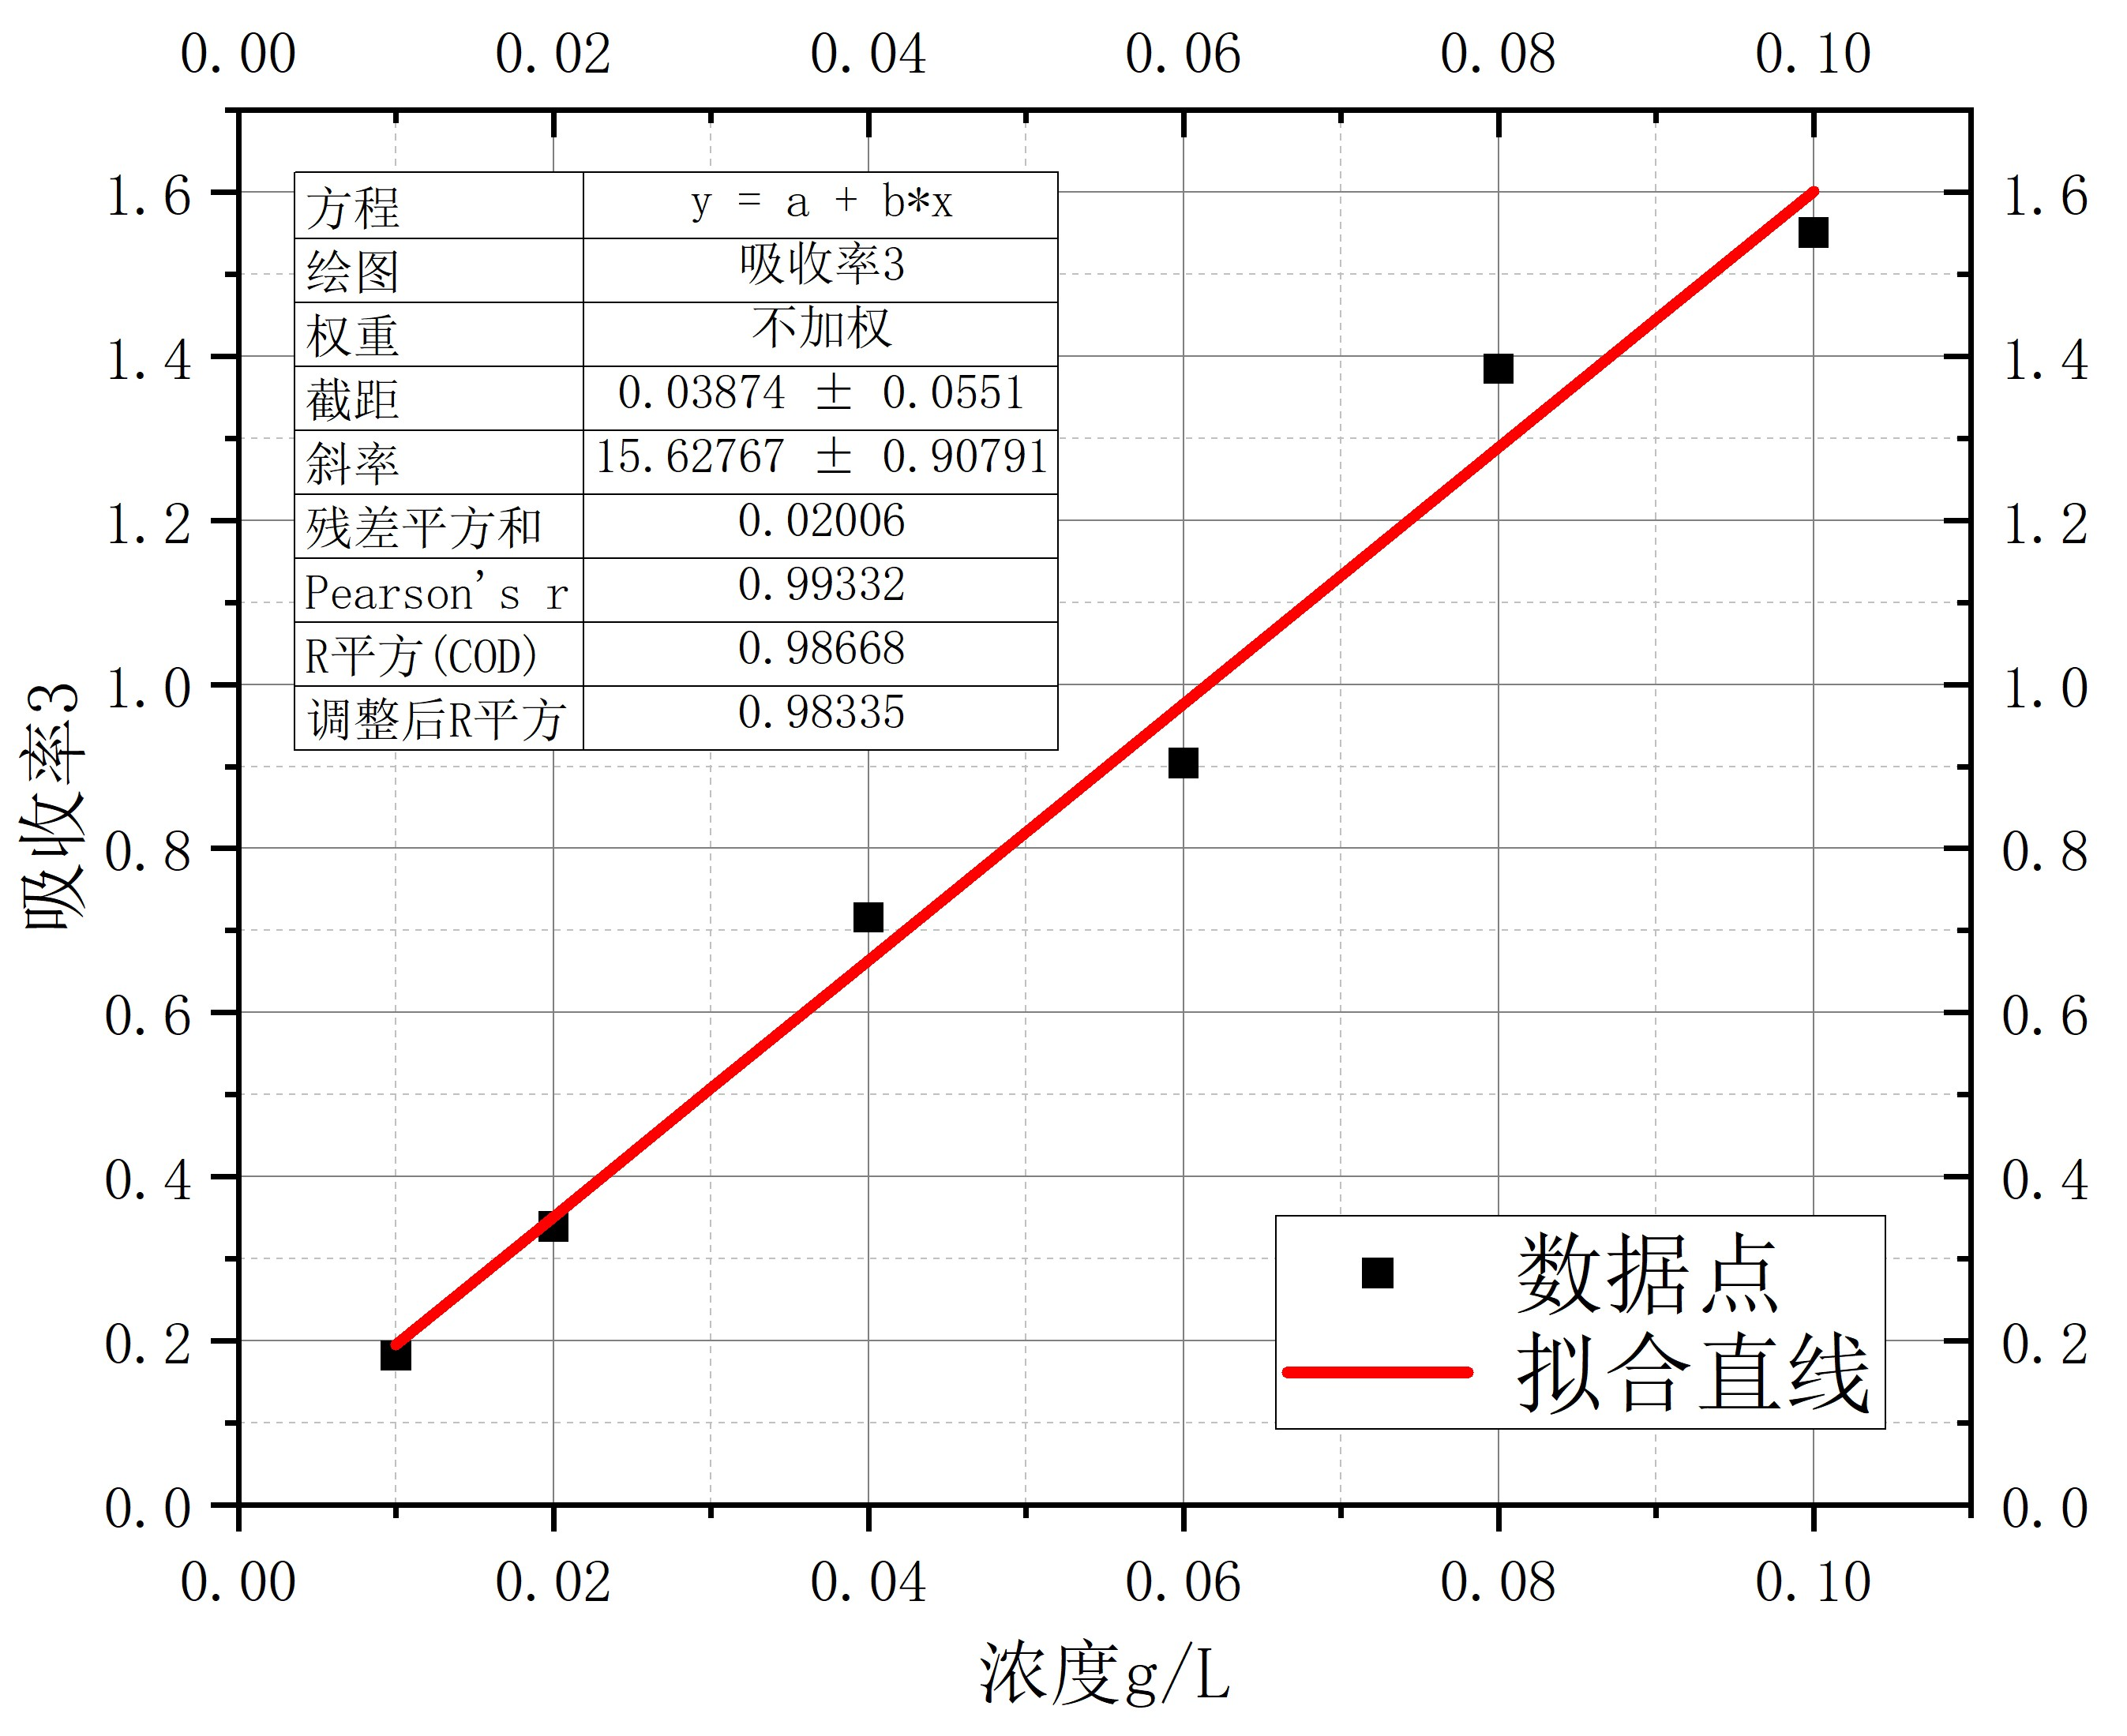
\includegraphics[width=0.55\textwidth]{Lab2_1Gra19.jpg}
		\caption{Beer定律验证3}
		\label{fig:fig19}
	\end{figure}
	
	上述分析当中良好的线性关系验证了Beer定律的成立。
	
	但是,值得注意的是,在紫外段出现了很明显不符合Beer定律的情况,即0.08g/L对应的吸收峰峰值高于0.1g/L的吸收峰峰值。
	
	%
	\subsubsection{Lambert定律验证}
	如\textbf{问题记录}部分所述,测量时有着较大的噪声,因此我用Python语言编写了脚本进行滤波并进一步处理数据,完整代码及运行结果详见Github(如果有需要的话老师可以联系我)。
	
	下面展示一次滤波结果和所有滤波结束后结果,如\cref{fig:fig20}和\cref{fig:fig21}所示。
	
	\begin{figure}[htbp]
		\centering
		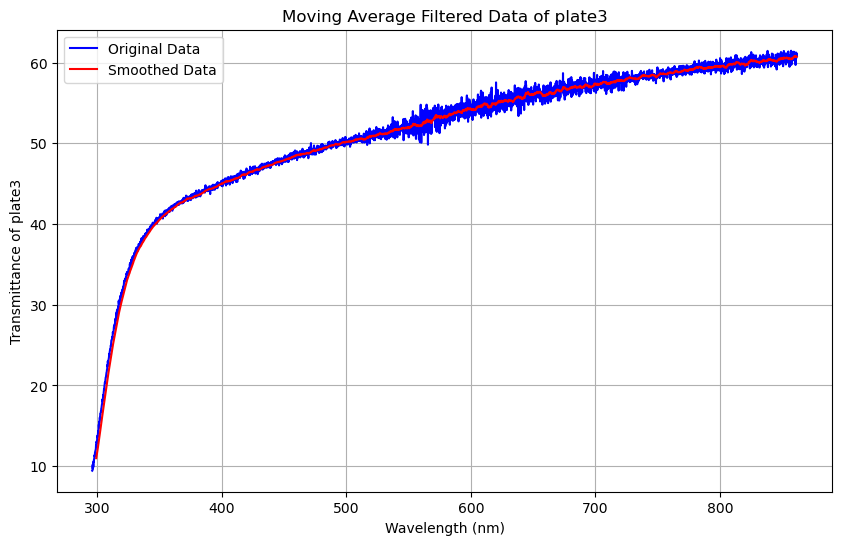
\includegraphics[width=0.5\textwidth]{Lab2_1Gra20.png}
		\caption{三层薄片一次滤波结果对比图}
		\label{fig:fig20}
	\end{figure}
	
	\begin{figure}[htbp]
		\centering
		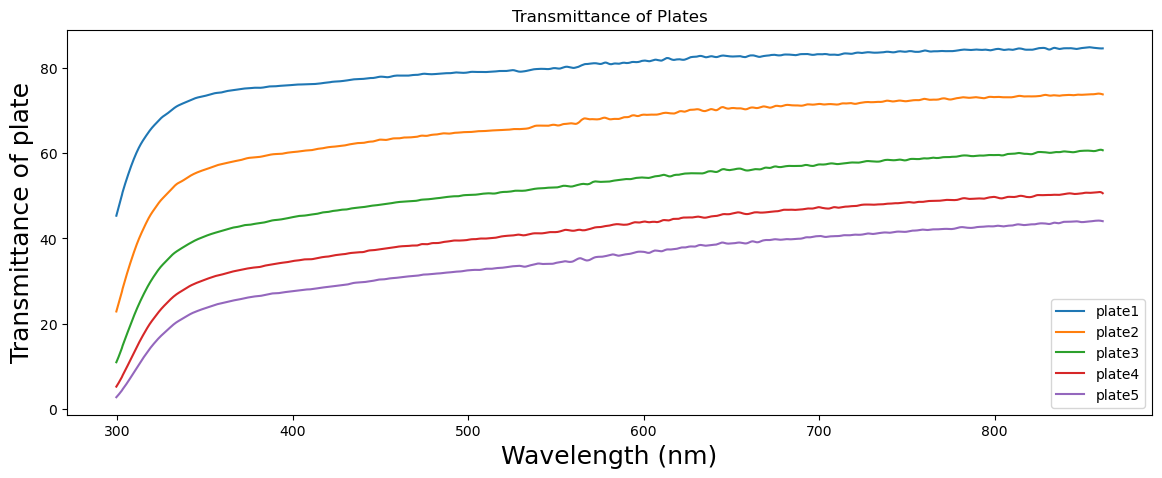
\includegraphics[width=0.75\textwidth]{Lab2_1Gra21.png}
		\caption{滤波后的完整数据图}
		\label{fig:fig21}
	\end{figure}
	
	利用滤波后数据,我取以平整阶段求平均透射率,结果如\cref{fig:fig22}所示。
	
	\begin{figure}[htbp]
		\centering
		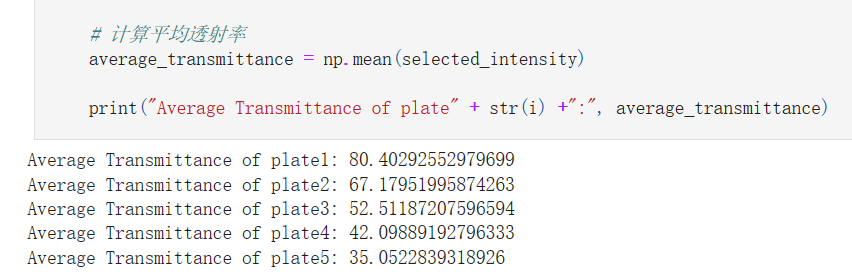
\includegraphics[width=0.45\textwidth]{Lab2_1Gra22.png}
		\caption{平均透射率}
		\label{fig:fig22}
	\end{figure}
	
	\textbf{取对数}后利用Origin进行拟合,得到如\cref{fig:fig23}所示结果。
	
	\begin{figure}[htbp]
		\centering
		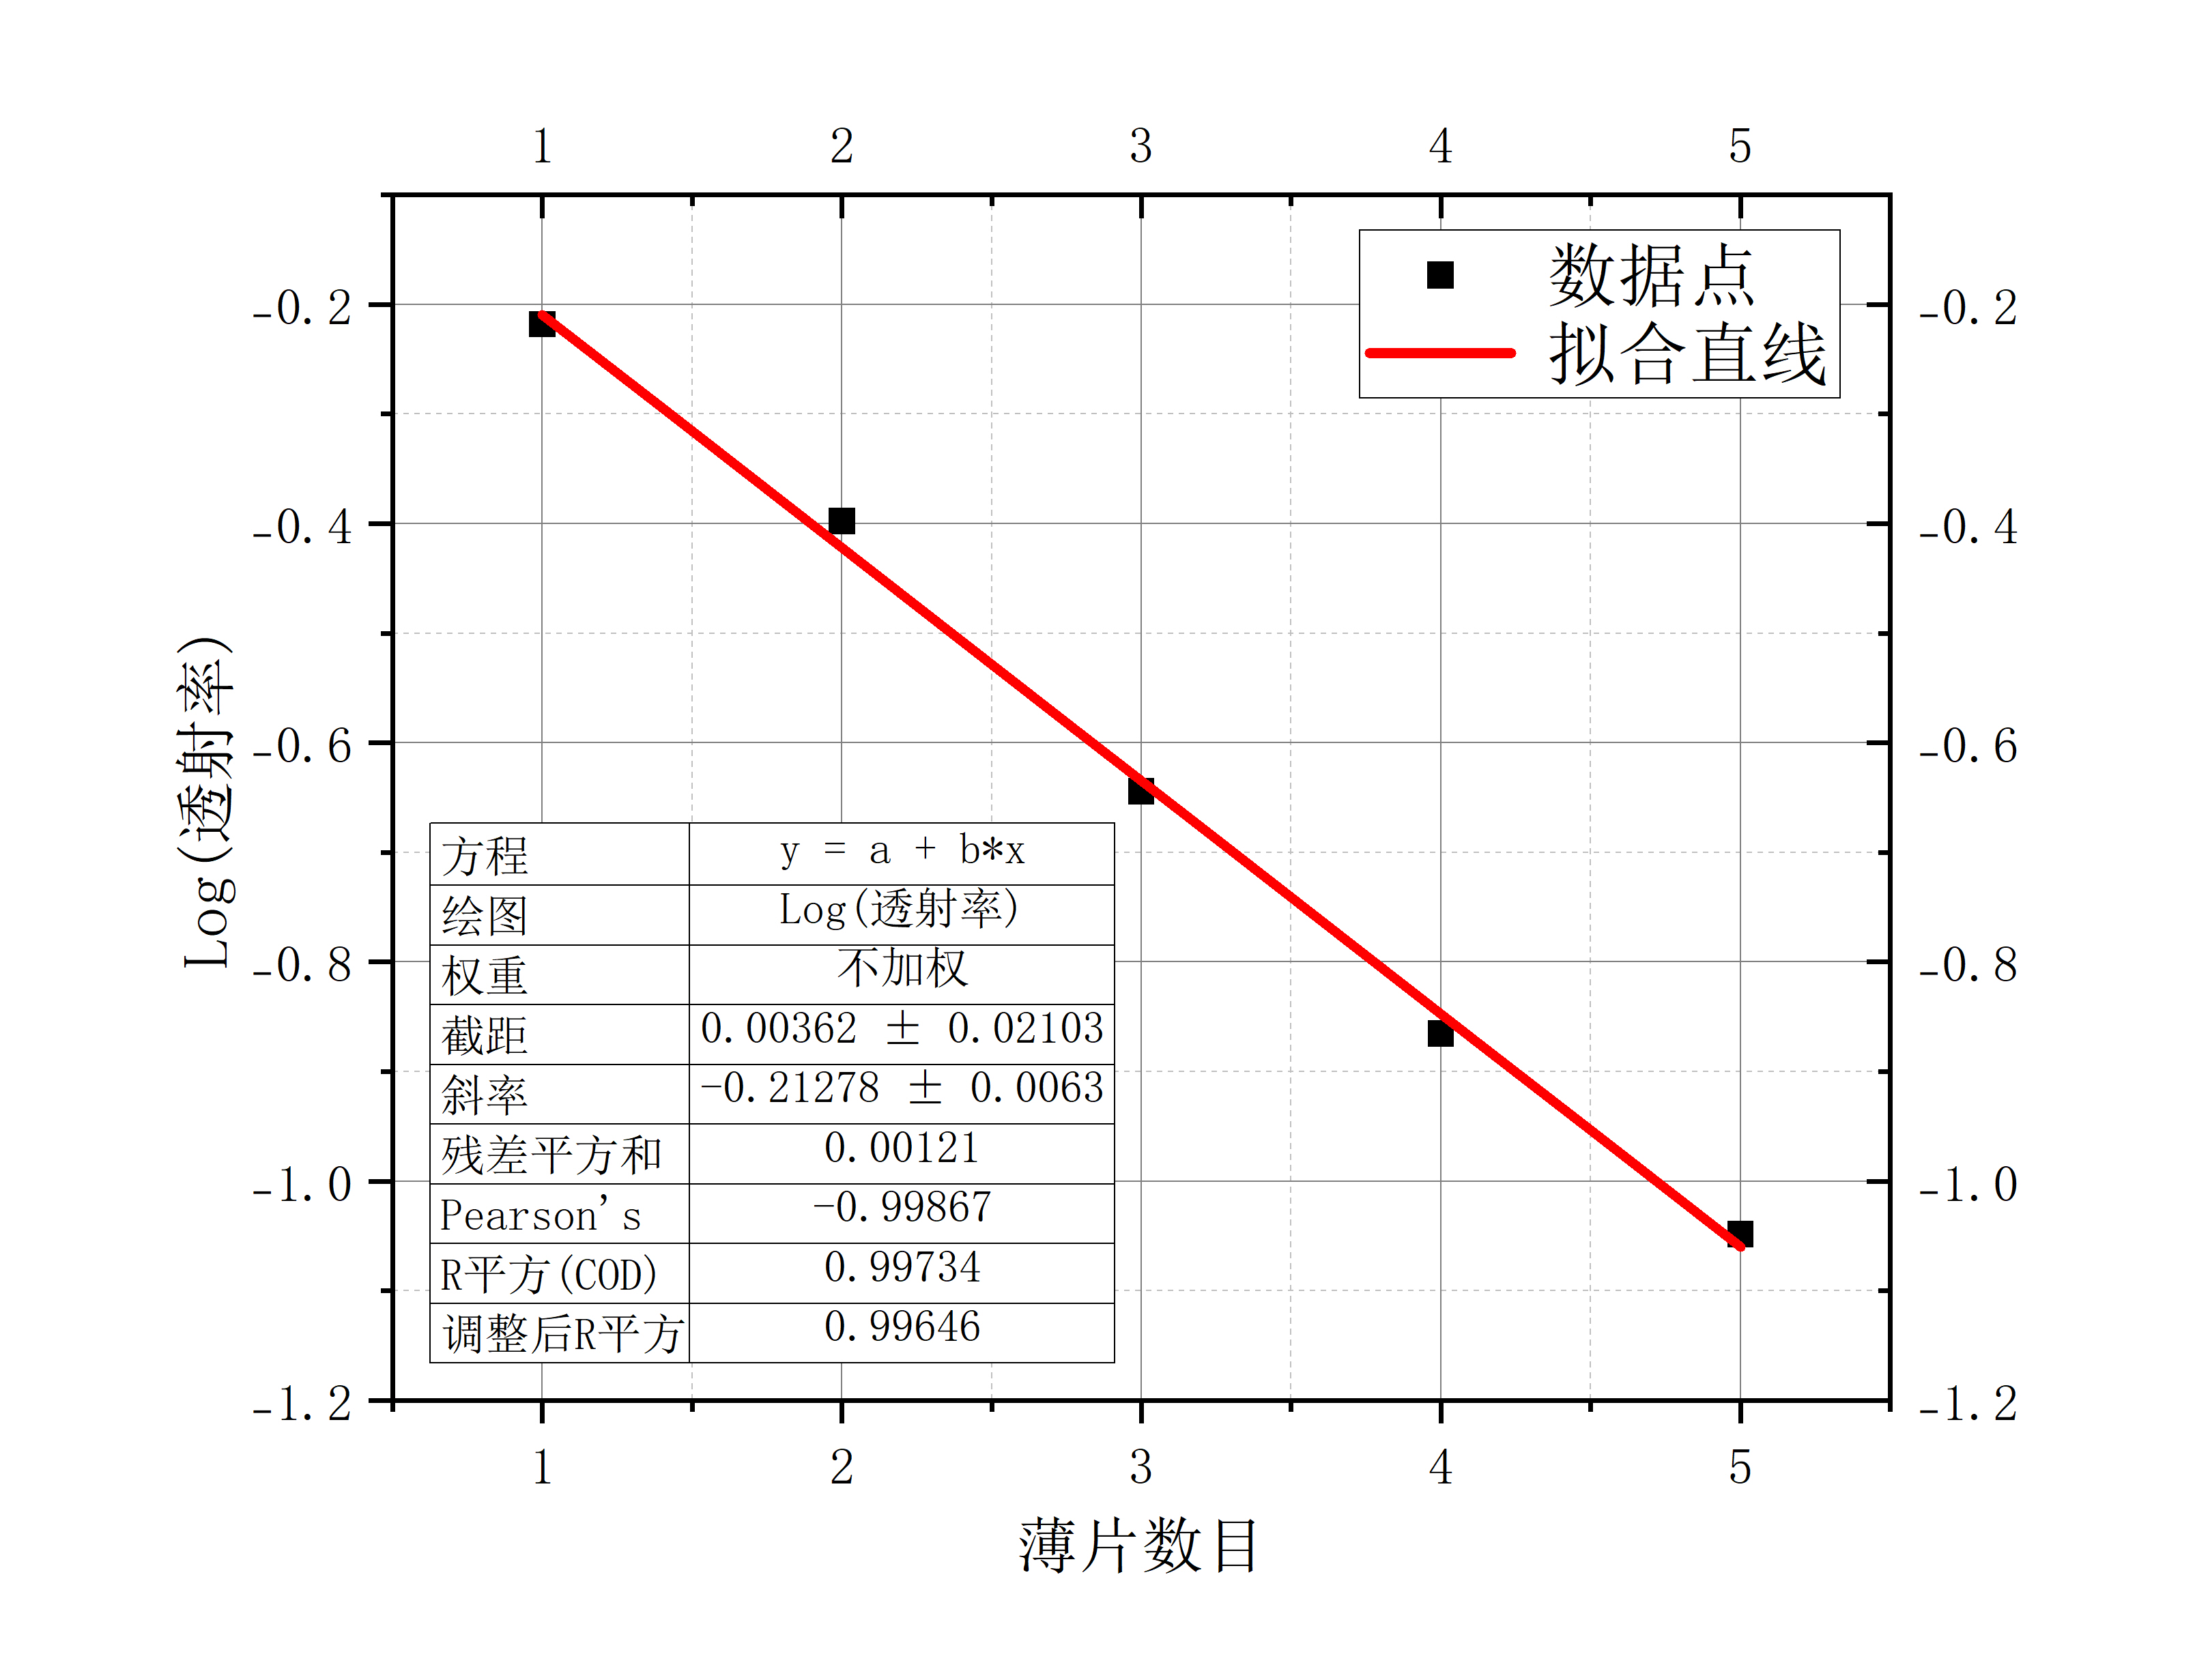
\includegraphics[width=0.7\textwidth]{Lab2_1Gra23.jpg}
		\caption{Lambert定律验证}
		\label{fig:fig23}
	\end{figure}
	
	从如中可以看出,斜率为负,而线性相关系数达到-0.998,这说明这些数据点有着相当好的线性关系,因此这验证了Lambert定律。
	
	% ---
	
	% 实验后思考题
	\subsection{实验后思考题}
	
	%思考题1
	\begin{question}
		钠灯光谱有哪些特征?能否从光谱图上判别各谱线所属线系?举例说明。
	\end{question}
	\begin{enumerate}
		\item 钠灯光谱的特征
		\begin{enumerate}
			\item \textbf{D线双峰:} 钠光谱中最著名的特征是其D线,它实际上是由两条非常接近的光谱线组成的,分别是D1线(波长约为589.6纳米)和D2线(波长约为589.0纳米)。这两条线是由钠原子的最外层电子从$3p$能级跃迁到$3s$能级时发射的。
			
			\item \textbf{线系:} 钠的光谱线可以根据其电子跃迁的起始和结束能级被分入不同的线系,如主线系(主要是$s$-$p$跃迁)、尖锐线系($p$-$d$跃迁)和扩散线系($d$-$f$跃迁)。每个线系的光谱线具有特定的能级差,因此具有特定的波长。
			
			\item \textbf{光谱线宽度:} 受多种因素影响,如温度、压力和原子间相互作用,光谱线的宽度可以提供有关钠灯内部条件的信息。
		\end{enumerate}
		
		\item 如何从光谱图上判别各谱线所属线系
		\begin{enumerate}
			\item \textbf{波长分析:} 通过测量光谱线的精确波长,可以与已知的钠原子跃迁能级进行比较,从而确定每条线的起始和结束能级,进而归属于特定的线系。一般来说,通过精确的光谱分析仪器,可以明确地区分不同的谱线并归属到特定的线系。例如,钠的光谱不仅包含D线,还包含许多其他线系的谱线,如钠的主线系(主要是D线)和其他线系,如共振线、尖锐线等。每个线系的谱线对应于钠原子内电子从一个特定能级跃迁到另一个能级时发射或吸收的光波长。
			
			\item \textbf{相对强度:} 不同线系中的光谱线由于跃迁概率不同,其相对强度也不同。这可以用于辅助识别线系,特别是在具有大量光谱线的复杂光谱中。
			
			\item \textbf{实验条件对比:} 改变实验条件(如温度、压力)可能会影响特定线系中光谱线的相对强度,通过对比这些变化,有助于判别线系。典型的高压钠灯的色温约为2100K,具有黄色光源色,但通过改进可以达到更高的色温和更好的色彩再现指数。例如,通过增加钠蒸气压力和改变放电管中汞与钠的比例,可以得到色温高达4000K,色彩再现指数接近88的新型钠灯 。
		\end{enumerate}
		
		\item 举例说明
		\begin{enumerate}
			\item 以D线为例,由于D1和D2线非常接近且分别对应于$3p$到$3s$能级的跃迁,通过波长测量可以准确地将它们归类为主线系。实验中,通过精确测量这两条线的波长并与理论值进行比较,可以确认它们的存在并归属于主线系。
			\item 通过高分辨率的光谱图,我们可以观察到除了D线之外,还可能观察到钠的其他谱线,如在330.3 nm的尖锐线(Sharp line)或在818.3 nm和819.5 nm处的红外线。每条谱线的存在都揭示了钠原子内部电子跃迁的具体过程,通过分析这些谱线的特征,可以进一步了解钠原子的电子结构和能级分布。
			\item 在高压钠灯的光谱中,由于钠的密度相对较高,钠D线的轮廓被扩展到足以覆盖大部分光谱。这种扩展是由固有线宽增加和自吸收引起的。特别地,高压钠灯的发射光谱中观察到的特征连续结构,例如在882nm附近的卫星带,可以被解释为来自$1 ^3\Sigma^+_g - 1 ^3\Sigma^+_u$跃迁的卫星带。此外,与钠-汞系统类似,钠-镉(NaCd)激发子的可见光谱分析揭示了红色卫星带和扩散带的存在,这些光谱特征与钠D线的非常远红翼有关。
			
			从光谱图上判断各谱线所属的线系可能需要对特定的谱线特征有深入的理解。例如,通过观察特定的卫星带和扩散带的存在,可以识别出由特定元素或元素组合产生的谱线。如上所述,钠-镉(NaCd)激发子产生的红色卫星带就是一个明确的例子,这些带显示在691、697、709和726.5nm处,其存在为钠D线由镉引起的非常远红翼的复杂结构提供了解释。
			
		\end{enumerate}
	\end{enumerate}
	
	% 思考题2
	\begin{question}
		在发射光谱和吸收光谱测量中,光路有何异同?
	\end{question}
	\begin{enumerate}
		\item 发射光谱的光路
		
		在观测原子发射光谱时,实验的设置主要关注如何有效地捕获和分析由原子发射的光。这通常涉及将光源(如低压汞灯、低压钠灯、氢氘灯、溴钨灯等)置于实验装置中,使其发出的光通过一个或多个光学元件(如滤光片、光纤、分光器等),最终由光谱仪(例如,光纤光谱仪)捕捉并分析。在这种设置中,光源直接产生待测量的光谱,因此实验关注点在于如何有效地收集和分析这些光信号。
		
		\item 吸收光谱的光路
		
		在观测原子吸收光谱时,光路设置涉及光源、样品和光谱仪三个主要组成部分。光源(例如低压汞灯或溴钨灯)产生的光首先穿过包含待测物质的样品(如高锰酸钾溶液),样品中的原子或分子吸收特定波长的光,然后剩余的光被光谱仪捕获并分析。在这种设置中,光路设计要确保来自光源的光均匀地穿过样品,并且能够有效地收集样品吸收后的光信号。
		
		\item 异同点
		\begin{itemize}
			\item \textbf{相同点:} 无论是发射光谱还是吸收光谱测量,光路中都会涉及光源、样品(在发射光谱测量中样品直接作为光源或位于光源附近),以及用于捕获和分析光信号的光谱仪。
			\item \textbf{不同点:} 在发射光谱测量中,光源产生的光直接被光谱仪捕捉;而在吸收光谱测量中,光源产生的光首先通过样品,样品中的原子或分子吸收特定波长的光,然后剩余的光被光谱仪捕获。因此,吸收光谱的光路设计需要特别注意光源到样品再到光谱仪的路径安排,以确保光线能够有效穿过样品并被光谱仪捕获。
		\end{itemize}
	\end{enumerate}
	
	% 思考题3
	\begin{question}
		根据高锰酸钾溶液的吸收光谱, 应如何选择理想光源,为什么?
	\end{question}
	\begin{enumerate}
		\item 高锰酸钾($KMnO_4$)溶液的吸收光谱主要特征是在可见光区域有一个很强的吸收峰,尤其是在绿色光的波长范围内,大约在520到550纳米之间。这个强烈的吸收带导致高锰酸钾溶液呈现出其特征的深紫色。基于这一特征,选择理想光源时需要考虑以下因素:
		
		\begin{enumerate}
			\item \textbf{光源的光谱输出:} 理想的光源应当能够提供足够的强度覆盖高锰酸钾的主要吸收波长(520-550纳米)。这意味着光源应当在可见光范围内有一个宽广和均匀的发射谱,尤其是在高锰酸钾的吸收波长范围内。
			
			\item \textbf{光源稳定性:} 进行吸收光谱测量时,光源的稳定性至关重要,因为任何光强的波动都会直接影响到吸收值的测量精度。
			
			\item \textbf{光源的色温或波长选择:} 虽然理想光源应当覆盖高锰酸钾吸收峰的范围,但同时也要考虑其他波长的光能在实际应用中的用途,因为不同波长的光可能被溶液以不同程度吸收,从而影响最终测量结果的解析度和准确性。
		\end{enumerate}
		
		\item \textbf{理想光源的选择}
		
		基于以上考虑,以下类型的光源可能是理想选择:
		
		\begin{itemize}
			\item \textbf{卤素灯:} 卤素灯可以提供宽广而连续的光谱输出,包括覆盖高锰酸钾吸收峰的520-550纳米波长范围。它们的光输出相对稳定,适合用于精确的光谱测量。
			
			\item \textbf{白炽灯:} 虽然不如卤素灯稳定和效率高,但白炽灯同样能提供连续的光谱输出,覆盖可见光范围。
			
			\item \textbf{LED光源:} 特定波长的LED可以用于更精确的吸收测量,尤其是如果能够获取到与高锰酸钾吸收峰匹配的波长。LED光源的优点包括高效率、长寿命和稳定的输出。但是,选择LED时需注意选择正确的波长以匹配吸收峰。
		\end{itemize}
		
		\item \textbf{为什么选择这样的光源}
		
		选择理想光源的关键是确保在高锰酸钾溶液的强吸收区域有足够的光强度差异,以便进行有效的吸收测量。光源应该能够提供稳定而均匀的照明,覆盖高锰酸钾的主要吸收波长,从而最大化测量灵敏度和准确性。这样的光源选择有助于确保在分析化学中进行精确的定量分析,提高实验数据的可靠性和重复性。
	\end{enumerate}
	
	% ---
	
	
	% 结语部分
	\clearpage
	
	% 小标题
	\section{Lab2-1 原子的发射和吸收光谱观测分析实验 \quad\heiti 结语}
	% ---
	
	% 总结、杂谈与致谢
	\subsection{总结、杂谈与致谢}
	\begin{enumerate}
		\item 这个实验的实验过程比较简单,但实验报告非常难写。
		\item 在写实验报告过程中,我提升了自己的数据处理能力(这是我首次用滤波器处理数据)。
		\item 感谢老师能阅读这篇还有很多不足的实验报告,希望老师能指出做得不好的地方;祝老师身体健康、生活幸福、工作顺利!
	\end{enumerate}
	% ---
	
	% 参考文献
	\subsection{参考文献}
	[1] 维基百科 https://zh.wikipedia.org
	
	[2] 沈韩.基础物理实验.——北京:科学出版社,2015.2 ISBN:978-7-03-043311-4
	
	[3] 相关实验报告
	
	% ---
	
	% 附件
	\subsection{附件}
%	试验台桌面整理如%\cref{}所示。
	
	实验报告\textbf{个人签名}如\cref{fig:name}。
	
	\begin{figure}[htbp]
		\centering
		
\includegraphics[width=0.7\textwidth]{name.png}
		\caption{个人签名}
		\label{fig:name}
	\end{figure}
	
	% ---
	
	相关代码已上传至Github。
	
	
	
\end{document}